\documentclass[twoside]{book}

% Packages required by doxygen
\usepackage{calc}
\usepackage{doxygen}
\usepackage{graphicx}
\usepackage[utf8]{inputenc}
\usepackage{makeidx}
\usepackage{multicol}
\usepackage{multirow}
\usepackage{fixltx2e}
\PassOptionsToPackage{warn}{textcomp}
\usepackage{textcomp}
\usepackage[nointegrals]{wasysym}
\usepackage[table]{xcolor}

% NLS support packages
\usepackage[french]{babel}

% Font selection
\usepackage[T1]{fontenc}
\usepackage{mathptmx}
\usepackage[scaled=.90]{helvet}
\usepackage{courier}
\usepackage{amssymb}
\usepackage{sectsty}
\renewcommand{\familydefault}{\sfdefault}
\allsectionsfont{%
  \fontseries{bc}\selectfont%
  \color{darkgray}%
}
\renewcommand{\DoxyLabelFont}{%
  \fontseries{bc}\selectfont%
  \color{darkgray}%
}
\newcommand{\+}{\discretionary{\mbox{\scriptsize$\hookleftarrow$}}{}{}}

% Page & text layout
\usepackage{geometry}
\geometry{%
  a4paper,%
  top=2.5cm,%
  bottom=2.5cm,%
  left=2.5cm,%
  right=2.5cm%
}
\tolerance=750
\hfuzz=15pt
\hbadness=750
\setlength{\emergencystretch}{15pt}
\setlength{\parindent}{0cm}
\setlength{\parskip}{0.2cm}
\makeatletter
\renewcommand{\paragraph}{%
  \@startsection{paragraph}{4}{0ex}{-1.0ex}{1.0ex}{%
    \normalfont\normalsize\bfseries\SS@parafont%
  }%
}
\renewcommand{\subparagraph}{%
  \@startsection{subparagraph}{5}{0ex}{-1.0ex}{1.0ex}{%
    \normalfont\normalsize\bfseries\SS@subparafont%
  }%
}
\makeatother

% Headers & footers
\usepackage{fancyhdr}
\pagestyle{fancyplain}
\fancyhead[LE]{\fancyplain{}{\bfseries\thepage}}
\fancyhead[CE]{\fancyplain{}{}}
\fancyhead[RE]{\fancyplain{}{\bfseries\leftmark}}
\fancyhead[LO]{\fancyplain{}{\bfseries\rightmark}}
\fancyhead[CO]{\fancyplain{}{}}
\fancyhead[RO]{\fancyplain{}{\bfseries\thepage}}
\fancyfoot[LE]{\fancyplain{}{}}
\fancyfoot[CE]{\fancyplain{}{}}
\fancyfoot[RE]{\fancyplain{}{\bfseries\scriptsize Généré le Mercredi 11 Juin 2014 22\+:26\+:13 pour U\+T\+Profiler par Doxygen }}
\fancyfoot[LO]{\fancyplain{}{\bfseries\scriptsize Généré le Mercredi 11 Juin 2014 22\+:26\+:13 pour U\+T\+Profiler par Doxygen }}
\fancyfoot[CO]{\fancyplain{}{}}
\fancyfoot[RO]{\fancyplain{}{}}
\renewcommand{\footrulewidth}{0.4pt}
\renewcommand{\chaptermark}[1]{%
  \markboth{#1}{}%
}
\renewcommand{\sectionmark}[1]{%
  \markright{\thesection\ #1}%
}

% Indices & bibliography
\usepackage{natbib}
\usepackage[titles]{tocloft}
\setcounter{tocdepth}{3}
\setcounter{secnumdepth}{5}
\makeindex

% Hyperlinks (required, but should be loaded last)
\usepackage{ifpdf}
\ifpdf
  \usepackage[pdftex,pagebackref=true]{hyperref}
\else
  \usepackage[ps2pdf,pagebackref=true]{hyperref}
\fi
\hypersetup{%
  colorlinks=true,%
  linkcolor=blue,%
  citecolor=blue,%
  unicode%
}

% Custom commands
\newcommand{\clearemptydoublepage}{%
  \newpage{\pagestyle{empty}\cleardoublepage}%
}


%===== C O N T E N T S =====

\begin{document}

% Titlepage & ToC
\hypersetup{pageanchor=false,
             bookmarks=true,
             bookmarksnumbered=true,
             pdfencoding=unicode
            }
\pagenumbering{roman}
\begin{titlepage}
\vspace*{7cm}
\begin{center}%
{\Large U\+T\+Profiler \\[1ex]\large 1.\+0 }\\
\vspace*{1cm}
{\large Généré par Doxygen 1.8.7}\\
\vspace*{0.5cm}
{\small Mercredi 11 Juin 2014 22:26:13}\\
\end{center}
\end{titlepage}
\clearemptydoublepage
\tableofcontents
\clearemptydoublepage
\pagenumbering{arabic}
\hypersetup{pageanchor=true}

%--- Begin generated contents ---
\chapter{Index hiérarchique}
\section{Hiérarchie des classes}
Cette liste d'héritage est classée approximativement par ordre alphabétique \+:\begin{DoxyCompactList}
\item \contentsline{section}{Dossier}{\pageref{class_dossier}}{}
\item exception\begin{DoxyCompactList}
\item \contentsline{section}{Formulaire\+Exception}{\pageref{class_formulaire_exception}}{}
\end{DoxyCompactList}
\item \contentsline{section}{Fenêtre}{\pageref{class_fen_xC3_xAAtre}}{}
\item \contentsline{section}{U\+V\+Manager\+:\+:Filter\+Iterator}{\pageref{class_u_v_manager_1_1_filter_iterator}}{}
\item \contentsline{section}{Formation}{\pageref{class_formation}}{}
\item \contentsline{section}{formulaire$<$ T $>$}{\pageref{classformulaire}}{}
\item \contentsline{section}{U\+V\+Manager\+:\+:Iterator}{\pageref{class_u_v_manager_1_1_iterator}}{}
\item \contentsline{section}{U\+V\+Manager\+:\+:iterator}{\pageref{class_u_v_manager_1_1iterator}}{}
\item \contentsline{section}{Note}{\pageref{class_note}}{}
\item Q\+Dialog\begin{DoxyCompactList}
\item \contentsline{section}{afficherchoixprev}{\pageref{classafficherchoixprev}}{}
\item \contentsline{section}{Inscription}{\pageref{class_inscription}}{}
\item \contentsline{section}{mondossier}{\pageref{classmondossier}}{}
\end{DoxyCompactList}
\item Q\+Frame\begin{DoxyCompactList}
\item \contentsline{section}{Administration}{\pageref{class_administration}}{}
\item \contentsline{section}{choixprevisionnel}{\pageref{classchoixprevisionnel}}{}
\end{DoxyCompactList}
\item Q\+Main\+Window\begin{DoxyCompactList}
\item \contentsline{section}{Accueil}{\pageref{class_accueil}}{}
\end{DoxyCompactList}
\item \contentsline{section}{qt\+\_\+meta\+\_\+stringdata\+\_\+\+Accueil\+\_\+t}{\pageref{structqt__meta__stringdata___accueil__t}}{}
\item \contentsline{section}{qt\+\_\+meta\+\_\+stringdata\+\_\+\+Administration\+\_\+t}{\pageref{structqt__meta__stringdata___administration__t}}{}
\item \contentsline{section}{qt\+\_\+meta\+\_\+stringdata\+\_\+detailuv\+\_\+t}{\pageref{structqt__meta__stringdata__detailuv__t}}{}
\item \contentsline{section}{qt\+\_\+meta\+\_\+stringdata\+\_\+fenetreplus\+\_\+t}{\pageref{structqt__meta__stringdata__fenetreplus__t}}{}
\item \contentsline{section}{qt\+\_\+meta\+\_\+stringdata\+\_\+\+Inscription\+\_\+t}{\pageref{structqt__meta__stringdata___inscription__t}}{}
\item \contentsline{section}{qt\+\_\+meta\+\_\+stringdata\+\_\+\+Insert\+Uv\+\_\+t}{\pageref{structqt__meta__stringdata___insert_uv__t}}{}
\item \contentsline{section}{qt\+\_\+meta\+\_\+stringdata\+\_\+mondossier\+\_\+t}{\pageref{structqt__meta__stringdata__mondossier__t}}{}
\item \contentsline{section}{qt\+\_\+meta\+\_\+stringdata\+\_\+\+View\+Uv\+\_\+t}{\pageref{structqt__meta__stringdata___view_uv__t}}{}
\item Q\+Widget\begin{DoxyCompactList}
\item \contentsline{section}{detailuv}{\pageref{classdetailuv}}{}
\item \contentsline{section}{fenetreplus}{\pageref{classfenetreplus}}{}
\item \contentsline{section}{Insert\+Uv}{\pageref{class_insert_uv}}{}
\item \contentsline{section}{View\+Uv}{\pageref{class_view_uv}}{}
\end{DoxyCompactList}
\item \contentsline{section}{Singleton$<$ T $>$}{\pageref{class_singleton}}{}
\item \contentsline{section}{Singleton$<$ Branches $>$}{\pageref{class_singleton}}{}
\begin{DoxyCompactList}
\item \contentsline{section}{Branches}{\pageref{class_branches}}{}
\end{DoxyCompactList}
\item \contentsline{section}{Singleton$<$ Categorie $>$}{\pageref{class_singleton}}{}
\begin{DoxyCompactList}
\item \contentsline{section}{Categorie}{\pageref{class_categorie}}{}
\end{DoxyCompactList}
\item \contentsline{section}{Singleton$<$ Connexion $>$}{\pageref{class_singleton}}{}
\begin{DoxyCompactList}
\item \contentsline{section}{Connexion}{\pageref{class_connexion}}{}
\end{DoxyCompactList}
\item \contentsline{section}{Singleton$<$ Cursus $>$}{\pageref{class_singleton}}{}
\begin{DoxyCompactList}
\item \contentsline{section}{Cursus}{\pageref{class_cursus}}{}
\end{DoxyCompactList}
\item \contentsline{section}{Singleton$<$ dbmanager $>$}{\pageref{class_singleton}}{}
\begin{DoxyCompactList}
\item \contentsline{section}{dbmanager}{\pageref{classdbmanager}}{}
\end{DoxyCompactList}
\item \contentsline{section}{Singleton$<$ Disponibilites $>$}{\pageref{class_singleton}}{}
\begin{DoxyCompactList}
\item \contentsline{section}{Disponibilites}{\pageref{class_disponibilites}}{}
\end{DoxyCompactList}
\item \contentsline{section}{Singleton$<$ Etudiants $>$}{\pageref{class_singleton}}{}
\begin{DoxyCompactList}
\item \contentsline{section}{Etudiants}{\pageref{class_etudiants}}{}
\end{DoxyCompactList}
\item \contentsline{section}{Singleton$<$ Filieres $>$}{\pageref{class_singleton}}{}
\begin{DoxyCompactList}
\item \contentsline{section}{Filieres}{\pageref{class_filieres}}{}
\end{DoxyCompactList}
\item \contentsline{section}{Singleton$<$ Semestre $>$}{\pageref{class_singleton}}{}
\begin{DoxyCompactList}
\item \contentsline{section}{Semestre}{\pageref{class_semestre}}{}
\end{DoxyCompactList}
\item \contentsline{section}{Singleton$<$ uvmnger $>$}{\pageref{class_singleton}}{}
\begin{DoxyCompactList}
\item \contentsline{section}{uvmnger}{\pageref{classuvmnger}}{}
\end{DoxyCompactList}
\item \contentsline{section}{Tools}{\pageref{class_tools}}{}
\item \contentsline{section}{Ui\+\_\+\+Accueil}{\pageref{class_ui___accueil}}{}
\begin{DoxyCompactList}
\item \contentsline{section}{Ui\+:\+:Accueil}{\pageref{class_ui_1_1_accueil}}{}
\end{DoxyCompactList}
\item \contentsline{section}{Ui\+\_\+\+Administration}{\pageref{class_ui___administration}}{}
\begin{DoxyCompactList}
\item \contentsline{section}{Ui\+:\+:Administration}{\pageref{class_ui_1_1_administration}}{}
\end{DoxyCompactList}
\item \contentsline{section}{Ui\+\_\+afficherchoixprev}{\pageref{class_ui__afficherchoixprev}}{}
\begin{DoxyCompactList}
\item \contentsline{section}{Ui\+:\+:afficherchoixprev}{\pageref{class_ui_1_1afficherchoixprev}}{}
\end{DoxyCompactList}
\item \contentsline{section}{Ui\+\_\+detailuv}{\pageref{class_ui__detailuv}}{}
\begin{DoxyCompactList}
\item \contentsline{section}{Ui\+:\+:detailuv}{\pageref{class_ui_1_1detailuv}}{}
\end{DoxyCompactList}
\item \contentsline{section}{Ui\+\_\+fenetreplus}{\pageref{class_ui__fenetreplus}}{}
\begin{DoxyCompactList}
\item \contentsline{section}{Ui\+:\+:fenetreplus}{\pageref{class_ui_1_1fenetreplus}}{}
\end{DoxyCompactList}
\item \contentsline{section}{Ui\+\_\+\+Inscription}{\pageref{class_ui___inscription}}{}
\begin{DoxyCompactList}
\item \contentsline{section}{Ui\+:\+:Inscription}{\pageref{class_ui_1_1_inscription}}{}
\end{DoxyCompactList}
\item \contentsline{section}{Ui\+\_\+\+Insert\+Uv}{\pageref{class_ui___insert_uv}}{}
\begin{DoxyCompactList}
\item \contentsline{section}{Ui\+:\+:Insert\+Uv}{\pageref{class_ui_1_1_insert_uv}}{}
\end{DoxyCompactList}
\item \contentsline{section}{Ui\+\_\+mondossier}{\pageref{class_ui__mondossier}}{}
\begin{DoxyCompactList}
\item \contentsline{section}{Ui\+:\+:mondossier}{\pageref{class_ui_1_1mondossier}}{}
\end{DoxyCompactList}
\item \contentsline{section}{Ui\+\_\+\+View\+Uv}{\pageref{class_ui___view_uv}}{}
\begin{DoxyCompactList}
\item \contentsline{section}{Ui\+:\+:View\+Uv}{\pageref{class_ui_1_1_view_uv}}{}
\end{DoxyCompactList}
\item \contentsline{section}{U\+T\+Profiler\+Exception}{\pageref{class_u_t_profiler_exception}}{}
\item \contentsline{section}{U\+V}{\pageref{class_u_v}}{}
\item \contentsline{section}{U\+V\+Manager}{\pageref{class_u_v_manager}}{}
\end{DoxyCompactList}

\chapter{Index des classes}
\section{Liste des classes}
Liste des classes, structures, unions et interfaces avec une brève description \+:\begin{DoxyCompactList}
\item\contentsline{section}{\hyperlink{class_accueil}{Accueil} }{\pageref{class_accueil}}{}
\item\contentsline{section}{\hyperlink{class_ui_1_1_accueil}{Ui\+::\+Accueil} }{\pageref{class_ui_1_1_accueil}}{}
\item\contentsline{section}{\hyperlink{class_administration}{Administration} }{\pageref{class_administration}}{}
\item\contentsline{section}{\hyperlink{class_ui_1_1_administration}{Ui\+::\+Administration} }{\pageref{class_ui_1_1_administration}}{}
\item\contentsline{section}{\hyperlink{class_ui_1_1afficherchoixprev}{Ui\+::afficherchoixprev} }{\pageref{class_ui_1_1afficherchoixprev}}{}
\item\contentsline{section}{\hyperlink{classafficherchoixprev}{afficherchoixprev} }{\pageref{classafficherchoixprev}}{}
\item\contentsline{section}{\hyperlink{class_branches}{Branches} }{\pageref{class_branches}}{}
\item\contentsline{section}{\hyperlink{class_categorie}{Categorie} }{\pageref{class_categorie}}{}
\item\contentsline{section}{\hyperlink{classchoixprevisionnel}{choixprevisionnel} }{\pageref{classchoixprevisionnel}}{}
\item\contentsline{section}{\hyperlink{class_connexion}{Connexion} }{\pageref{class_connexion}}{}
\item\contentsline{section}{\hyperlink{class_cursus}{Cursus} }{\pageref{class_cursus}}{}
\item\contentsline{section}{\hyperlink{classdbmanager}{dbmanager} }{\pageref{classdbmanager}}{}
\item\contentsline{section}{\hyperlink{class_ui_1_1detailuv}{Ui\+::detailuv} }{\pageref{class_ui_1_1detailuv}}{}
\item\contentsline{section}{\hyperlink{classdetailuv}{detailuv} }{\pageref{classdetailuv}}{}
\item\contentsline{section}{\hyperlink{class_disponibilites}{Disponibilites} }{\pageref{class_disponibilites}}{}
\item\contentsline{section}{\hyperlink{class_dossier}{Dossier} }{\pageref{class_dossier}}{}
\item\contentsline{section}{\hyperlink{class_etudiants}{Etudiants} }{\pageref{class_etudiants}}{}
\item\contentsline{section}{\hyperlink{class_ui_1_1fenetreplus}{Ui\+::fenetreplus} }{\pageref{class_ui_1_1fenetreplus}}{}
\item\contentsline{section}{\hyperlink{classfenetreplus}{fenetreplus} }{\pageref{classfenetreplus}}{}
\item\contentsline{section}{\hyperlink{class_fen_xC3_xAAtre}{Fenêtre} }{\pageref{class_fen_xC3_xAAtre}}{}
\item\contentsline{section}{\hyperlink{class_filieres}{Filieres} }{\pageref{class_filieres}}{}
\item\contentsline{section}{\hyperlink{class_u_v_manager_1_1_filter_iterator}{U\+V\+Manager\+::\+Filter\+Iterator} }{\pageref{class_u_v_manager_1_1_filter_iterator}}{}
\item\contentsline{section}{\hyperlink{class_formation}{Formation} }{\pageref{class_formation}}{}
\item\contentsline{section}{\hyperlink{classformulaire}{formulaire$<$ T $>$} }{\pageref{classformulaire}}{}
\item\contentsline{section}{\hyperlink{class_formulaire_exception}{Formulaire\+Exception} }{\pageref{class_formulaire_exception}}{}
\item\contentsline{section}{\hyperlink{class_inscription}{Inscription} }{\pageref{class_inscription}}{}
\item\contentsline{section}{\hyperlink{class_ui_1_1_inscription}{Ui\+::\+Inscription} }{\pageref{class_ui_1_1_inscription}}{}
\item\contentsline{section}{\hyperlink{class_insert_uv}{Insert\+Uv} }{\pageref{class_insert_uv}}{}
\item\contentsline{section}{\hyperlink{class_ui_1_1_insert_uv}{Ui\+::\+Insert\+Uv} }{\pageref{class_ui_1_1_insert_uv}}{}
\item\contentsline{section}{\hyperlink{class_u_v_manager_1_1_iterator}{U\+V\+Manager\+::\+Iterator} }{\pageref{class_u_v_manager_1_1_iterator}}{}
\item\contentsline{section}{\hyperlink{class_u_v_manager_1_1iterator}{U\+V\+Manager\+::iterator} }{\pageref{class_u_v_manager_1_1iterator}}{}
\item\contentsline{section}{\hyperlink{class_ui_1_1mondossier}{Ui\+::mondossier} }{\pageref{class_ui_1_1mondossier}}{}
\item\contentsline{section}{\hyperlink{classmondossier}{mondossier} }{\pageref{classmondossier}}{}
\item\contentsline{section}{\hyperlink{class_note}{Note} }{\pageref{class_note}}{}
\item\contentsline{section}{\hyperlink{structqt__meta__stringdata___accueil__t}{qt\+\_\+meta\+\_\+stringdata\+\_\+\+Accueil\+\_\+t} }{\pageref{structqt__meta__stringdata___accueil__t}}{}
\item\contentsline{section}{\hyperlink{structqt__meta__stringdata___administration__t}{qt\+\_\+meta\+\_\+stringdata\+\_\+\+Administration\+\_\+t} }{\pageref{structqt__meta__stringdata___administration__t}}{}
\item\contentsline{section}{\hyperlink{structqt__meta__stringdata__detailuv__t}{qt\+\_\+meta\+\_\+stringdata\+\_\+detailuv\+\_\+t} }{\pageref{structqt__meta__stringdata__detailuv__t}}{}
\item\contentsline{section}{\hyperlink{structqt__meta__stringdata__fenetreplus__t}{qt\+\_\+meta\+\_\+stringdata\+\_\+fenetreplus\+\_\+t} }{\pageref{structqt__meta__stringdata__fenetreplus__t}}{}
\item\contentsline{section}{\hyperlink{structqt__meta__stringdata___inscription__t}{qt\+\_\+meta\+\_\+stringdata\+\_\+\+Inscription\+\_\+t} }{\pageref{structqt__meta__stringdata___inscription__t}}{}
\item\contentsline{section}{\hyperlink{structqt__meta__stringdata___insert_uv__t}{qt\+\_\+meta\+\_\+stringdata\+\_\+\+Insert\+Uv\+\_\+t} }{\pageref{structqt__meta__stringdata___insert_uv__t}}{}
\item\contentsline{section}{\hyperlink{structqt__meta__stringdata__mondossier__t}{qt\+\_\+meta\+\_\+stringdata\+\_\+mondossier\+\_\+t} }{\pageref{structqt__meta__stringdata__mondossier__t}}{}
\item\contentsline{section}{\hyperlink{structqt__meta__stringdata___view_uv__t}{qt\+\_\+meta\+\_\+stringdata\+\_\+\+View\+Uv\+\_\+t} }{\pageref{structqt__meta__stringdata___view_uv__t}}{}
\item\contentsline{section}{\hyperlink{class_semestre}{Semestre} }{\pageref{class_semestre}}{}
\item\contentsline{section}{\hyperlink{class_singleton}{Singleton$<$ T $>$} }{\pageref{class_singleton}}{}
\item\contentsline{section}{\hyperlink{class_tools}{Tools} }{\pageref{class_tools}}{}
\item\contentsline{section}{\hyperlink{class_ui___accueil}{Ui\+\_\+\+Accueil} }{\pageref{class_ui___accueil}}{}
\item\contentsline{section}{\hyperlink{class_ui___administration}{Ui\+\_\+\+Administration} }{\pageref{class_ui___administration}}{}
\item\contentsline{section}{\hyperlink{class_ui__afficherchoixprev}{Ui\+\_\+afficherchoixprev} }{\pageref{class_ui__afficherchoixprev}}{}
\item\contentsline{section}{\hyperlink{class_ui__detailuv}{Ui\+\_\+detailuv} }{\pageref{class_ui__detailuv}}{}
\item\contentsline{section}{\hyperlink{class_ui__fenetreplus}{Ui\+\_\+fenetreplus} }{\pageref{class_ui__fenetreplus}}{}
\item\contentsline{section}{\hyperlink{class_ui___inscription}{Ui\+\_\+\+Inscription} }{\pageref{class_ui___inscription}}{}
\item\contentsline{section}{\hyperlink{class_ui___insert_uv}{Ui\+\_\+\+Insert\+Uv} }{\pageref{class_ui___insert_uv}}{}
\item\contentsline{section}{\hyperlink{class_ui__mondossier}{Ui\+\_\+mondossier} }{\pageref{class_ui__mondossier}}{}
\item\contentsline{section}{\hyperlink{class_ui___view_uv}{Ui\+\_\+\+View\+Uv} }{\pageref{class_ui___view_uv}}{}
\item\contentsline{section}{\hyperlink{class_u_t_profiler_exception}{U\+T\+Profiler\+Exception} }{\pageref{class_u_t_profiler_exception}}{}
\item\contentsline{section}{\hyperlink{class_u_v}{U\+V} }{\pageref{class_u_v}}{}
\item\contentsline{section}{\hyperlink{class_u_v_manager}{U\+V\+Manager} }{\pageref{class_u_v_manager}}{}
\item\contentsline{section}{\hyperlink{classuvmnger}{uvmnger} }{\pageref{classuvmnger}}{}
\item\contentsline{section}{\hyperlink{class_ui_1_1_view_uv}{Ui\+::\+View\+Uv} }{\pageref{class_ui_1_1_view_uv}}{}
\item\contentsline{section}{\hyperlink{class_view_uv}{View\+Uv} }{\pageref{class_view_uv}}{}
\end{DoxyCompactList}

\chapter{Index des fichiers}
\section{Liste des fichiers}
Liste de tous les fichiers documentés avec une brève description \+:\begin{DoxyCompactList}
\item\contentsline{section}{\hyperlink{accueil_8cpp}{accueil.\+cpp} }{\pageref{accueil_8cpp}}{}
\item\contentsline{section}{\hyperlink{accueil_8h}{accueil.\+h} \\*Interface d'accueil de l'application }{\pageref{accueil_8h}}{}
\item\contentsline{section}{\hyperlink{administration_8cpp}{administration.\+cpp} }{\pageref{administration_8cpp}}{}
\item\contentsline{section}{\hyperlink{administration_8h}{administration.\+h} }{\pageref{administration_8h}}{}
\item\contentsline{section}{{\bfseries afficherchoixprev.\+h} }{\pageref{afficherchoixprev_8h}}{}
\item\contentsline{section}{{\bfseries branches.\+h} }{\pageref{branches_8h}}{}
\item\contentsline{section}{{\bfseries categorie.\+h} }{\pageref{categorie_8h}}{}
\item\contentsline{section}{{\bfseries choixprevisionnel.\+h} }{\pageref{choixprevisionnel_8h}}{}
\item\contentsline{section}{{\bfseries connexion.\+h} }{\pageref{connexion_8h}}{}
\item\contentsline{section}{{\bfseries cursus.\+h} }{\pageref{cursus_8h}}{}
\item\contentsline{section}{{\bfseries dbmanager.\+h} }{\pageref{dbmanager_8h}}{}
\item\contentsline{section}{{\bfseries detailuv.\+h} }{\pageref{detailuv_8h}}{}
\item\contentsline{section}{{\bfseries disponibilites.\+h} }{\pageref{disponibilites_8h}}{}
\item\contentsline{section}{{\bfseries etudiants.\+h} }{\pageref{etudiants_8h}}{}
\item\contentsline{section}{{\bfseries fenetreplus.\+h} }{\pageref{fenetreplus_8h}}{}
\item\contentsline{section}{{\bfseries filieres.\+h} }{\pageref{filieres_8h}}{}
\item\contentsline{section}{{\bfseries formulaire.\+h} }{\pageref{formulaire_8h}}{}
\item\contentsline{section}{{\bfseries inscription.\+h} }{\pageref{inscription_8h}}{}
\item\contentsline{section}{{\bfseries insertuv.\+h} }{\pageref{insertuv_8h}}{}
\item\contentsline{section}{\hyperlink{main_8cpp}{main.\+cpp} }{\pageref{main_8cpp}}{}
\item\contentsline{section}{{\bfseries mondossier.\+h} }{\pageref{mondossier_8h}}{}
\item\contentsline{section}{{\bfseries note.\+h} }{\pageref{note_8h}}{}
\item\contentsline{section}{{\bfseries semestre.\+h} }{\pageref{semestre_8h}}{}
\item\contentsline{section}{{\bfseries singleton.\+h} }{\pageref{singleton_8h}}{}
\item\contentsline{section}{{\bfseries tools.\+h} }{\pageref{tools_8h}}{}
\item\contentsline{section}{{\bfseries ui\+\_\+accueil.\+h} }{\pageref{ui__accueil_8h}}{}
\item\contentsline{section}{{\bfseries ui\+\_\+administration.\+h} }{\pageref{ui__administration_8h}}{}
\item\contentsline{section}{{\bfseries ui\+\_\+afficherchoixprev.\+h} }{\pageref{ui__afficherchoixprev_8h}}{}
\item\contentsline{section}{{\bfseries ui\+\_\+detailuv.\+h} }{\pageref{ui__detailuv_8h}}{}
\item\contentsline{section}{{\bfseries ui\+\_\+fenetreplus.\+h} }{\pageref{ui__fenetreplus_8h}}{}
\item\contentsline{section}{{\bfseries ui\+\_\+inscription.\+h} }{\pageref{ui__inscription_8h}}{}
\item\contentsline{section}{{\bfseries ui\+\_\+insertuv.\+h} }{\pageref{ui__insertuv_8h}}{}
\item\contentsline{section}{{\bfseries ui\+\_\+mondossier.\+h} }{\pageref{ui__mondossier_8h}}{}
\item\contentsline{section}{{\bfseries ui\+\_\+viewuv.\+h} }{\pageref{ui__viewuv_8h}}{}
\item\contentsline{section}{{\bfseries utprofilerexception.\+h} }{\pageref{utprofilerexception_8h}}{}
\item\contentsline{section}{{\bfseries uv.\+h} }{\pageref{uv_8h}}{}
\item\contentsline{section}{{\bfseries uvmanager.\+h} }{\pageref{uvmanager_8h}}{}
\item\contentsline{section}{{\bfseries uvmnger.\+h} }{\pageref{uvmnger_8h}}{}
\item\contentsline{section}{{\bfseries viewuv.\+h} }{\pageref{viewuv_8h}}{}
\end{DoxyCompactList}

\chapter{Documentation des classes}
\hypertarget{class_accueil}{\section{Référence de la classe Accueil}
\label{class_accueil}\index{Accueil@{Accueil}}
}
Graphe d'héritage de Accueil\+:\begin{figure}[H]
\begin{center}
\leavevmode
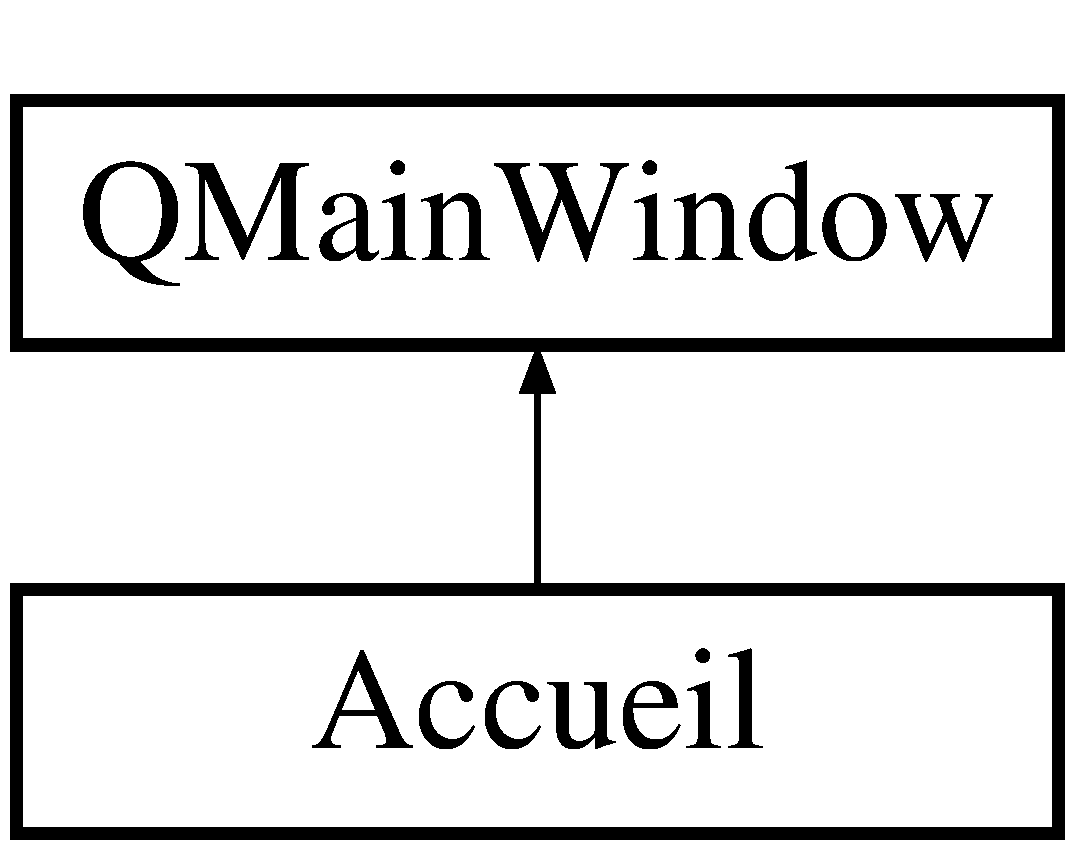
\includegraphics[height=2.000000cm]{class_accueil}
\end{center}
\end{figure}
\subsection*{Fonctions membres publiques}
\begin{DoxyCompactItemize}
\item 
\hyperlink{class_accueil_a581158b51548b6c3e60892035e9b656b}{Accueil} (Q\+Widget $\ast$parent=0)
\begin{DoxyCompactList}\small\item\em Constructeur de la classe \hyperlink{class_accueil}{Accueil}. \end{DoxyCompactList}\item 
\hypertarget{class_accueil_a42a925af8942c76a73957ac9abcd45d7}{\hyperlink{class_accueil_a42a925af8942c76a73957ac9abcd45d7}{$\sim$\+Accueil} ()}\label{class_accueil_a42a925af8942c76a73957ac9abcd45d7}

\begin{DoxyCompactList}\small\item\em Destructeur de la classe \hyperlink{class_accueil}{Accueil}. \end{DoxyCompactList}\end{DoxyCompactItemize}


\subsection{Documentation des constructeurs et destructeur}
\hypertarget{class_accueil_a581158b51548b6c3e60892035e9b656b}{\index{Accueil@{Accueil}!Accueil@{Accueil}}
\index{Accueil@{Accueil}!Accueil@{Accueil}}
\subsubsection[{Accueil}]{\setlength{\rightskip}{0pt plus 5cm}Accueil\+::\+Accueil (
\begin{DoxyParamCaption}
\item[{Q\+Widget $\ast$}]{parent = {\ttfamily 0}}
\end{DoxyParamCaption}
)\hspace{0.3cm}{\ttfamily [explicit]}}}\label{class_accueil_a581158b51548b6c3e60892035e9b656b}


Constructeur de la classe \hyperlink{class_accueil}{Accueil}. 


\begin{DoxyParams}{Paramètres}
{\em Q\+Widget} & $\ast$parent \\
\hline
\end{DoxyParams}
Création d'un nouvel onglet dans le tab\+Widget pour chaque cursus. Chaque onglet est composé d'un Groupbox pour la selection des critères de tri et d'un list\+Widget pour l'affichage des \hyperlink{class_u_v}{U\+V}

La documentation de cette classe a été générée à partir des fichiers suivants \+:\begin{DoxyCompactItemize}
\item 
\hyperlink{accueil_8h}{accueil.\+h}\item 
\hyperlink{accueil_8cpp}{accueil.\+cpp}\end{DoxyCompactItemize}

\hypertarget{class_ui_1_1_accueil}{\section{Référence de la classe Ui\+:\+:Accueil}
\label{class_ui_1_1_accueil}\index{Ui\+::\+Accueil@{Ui\+::\+Accueil}}
}
Graphe d'héritage de Ui\+:\+:Accueil\+:\begin{figure}[H]
\begin{center}
\leavevmode
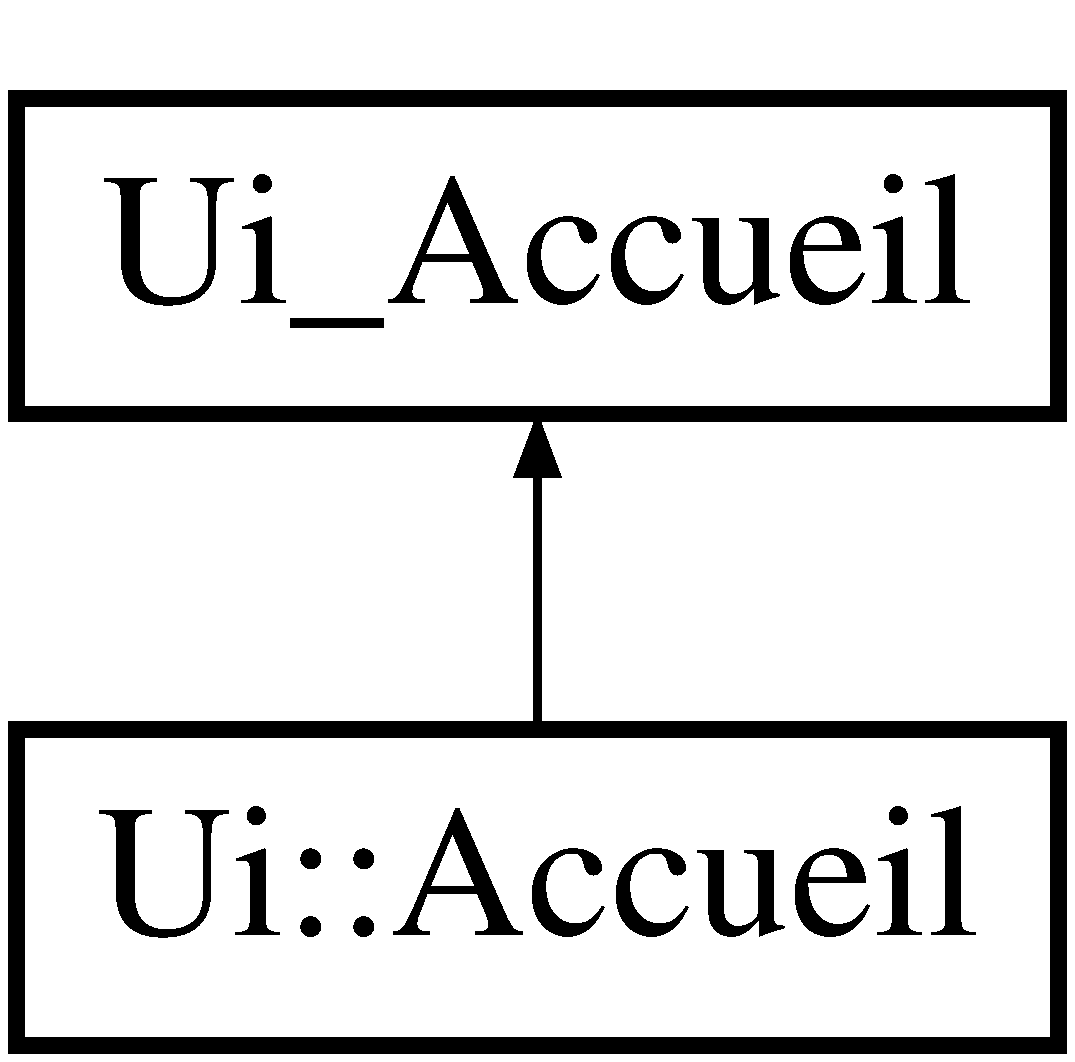
\includegraphics[height=2.000000cm]{class_ui_1_1_accueil}
\end{center}
\end{figure}
\subsection*{Membres hérités additionnels}


La documentation de cette classe a été générée à partir du fichier suivant \+:\begin{DoxyCompactItemize}
\item 
ui\+\_\+accueil.\+h\end{DoxyCompactItemize}

\hypertarget{class_administration}{\section{Référence de la classe Administration}
\label{class_administration}\index{Administration@{Administration}}
}
Graphe d'héritage de Administration\+:\begin{figure}[H]
\begin{center}
\leavevmode
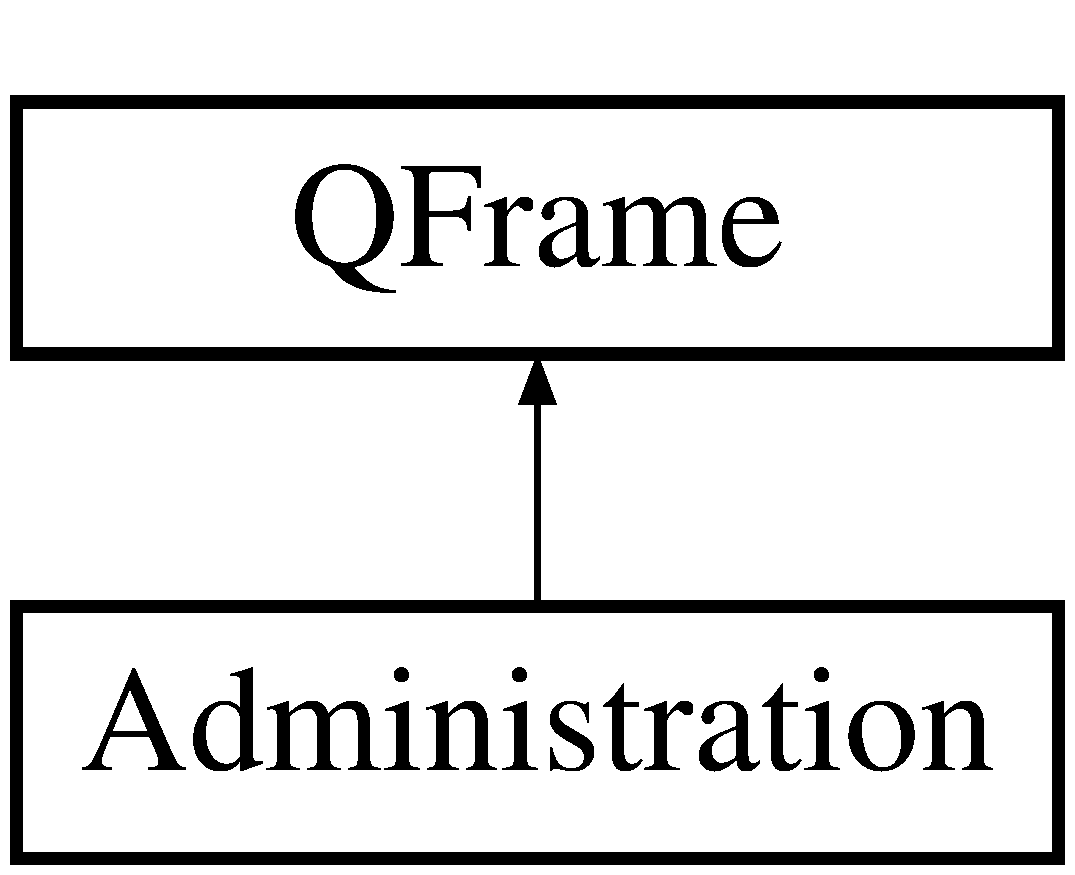
\includegraphics[height=2.000000cm]{class_administration}
\end{center}
\end{figure}
\subsection*{Fonctions membres publiques}
\begin{DoxyCompactItemize}
\item 
\hyperlink{class_administration_add46afefca972506093ce16385217f66}{Administration} (Q\+Widget $\ast$parent=0)
\begin{DoxyCompactList}\small\item\em Constructeur de la classe \hyperlink{class_administration}{Administration}. \end{DoxyCompactList}\end{DoxyCompactItemize}


\subsection{Documentation des constructeurs et destructeur}
\hypertarget{class_administration_add46afefca972506093ce16385217f66}{\index{Administration@{Administration}!Administration@{Administration}}
\index{Administration@{Administration}!Administration@{Administration}}
\subsubsection[{Administration}]{\setlength{\rightskip}{0pt plus 5cm}Administration\+::\+Administration (
\begin{DoxyParamCaption}
\item[{Q\+Widget $\ast$}]{parent = {\ttfamily 0}}
\end{DoxyParamCaption}
)\hspace{0.3cm}{\ttfamily [explicit]}}}\label{class_administration_add46afefca972506093ce16385217f66}


Constructeur de la classe \hyperlink{class_administration}{Administration}. 


\begin{DoxyParams}{Paramètres}
{\em Q\+Widget} & $\ast$parent \\
\hline
\end{DoxyParams}


La documentation de cette classe a été générée à partir des fichiers suivants \+:\begin{DoxyCompactItemize}
\item 
\hyperlink{administration_8h}{administration.\+h}\item 
\hyperlink{administration_8cpp}{administration.\+cpp}\end{DoxyCompactItemize}

\hypertarget{class_ui_1_1_administration}{\section{Référence de la classe Ui\+:\+:Administration}
\label{class_ui_1_1_administration}\index{Ui\+::\+Administration@{Ui\+::\+Administration}}
}
Graphe d'héritage de Ui\+:\+:Administration\+:\begin{figure}[H]
\begin{center}
\leavevmode
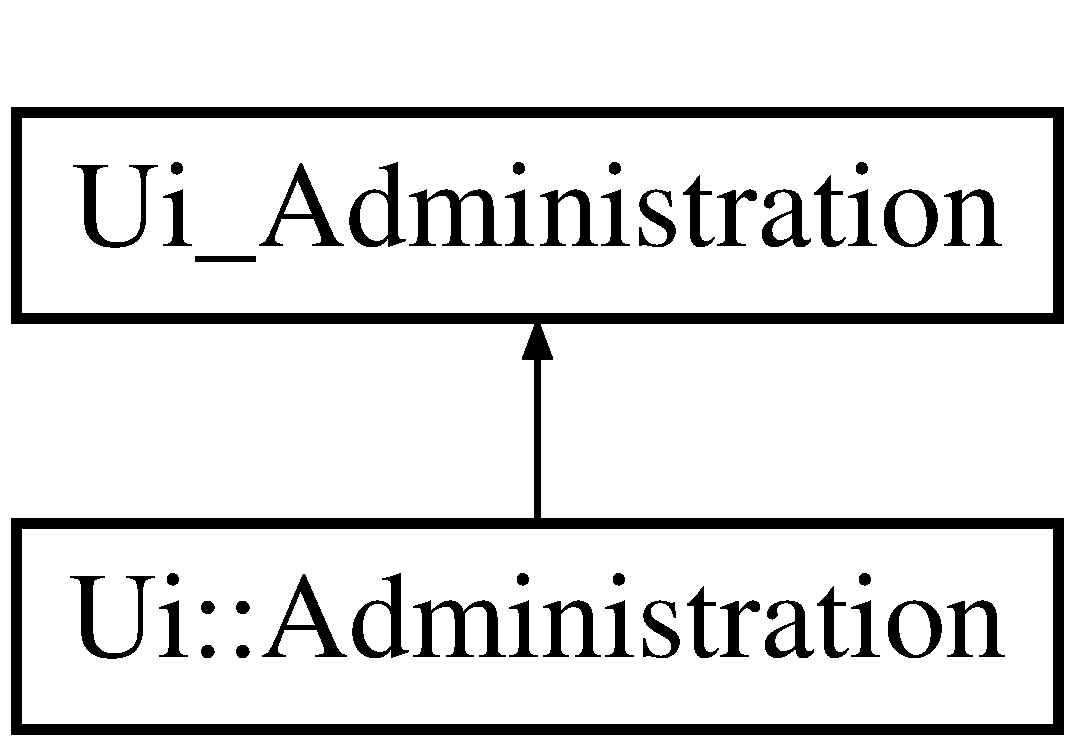
\includegraphics[height=2.000000cm]{class_ui_1_1_administration}
\end{center}
\end{figure}
\subsection*{Membres hérités additionnels}


La documentation de cette classe a été générée à partir du fichier suivant \+:\begin{DoxyCompactItemize}
\item 
ui\+\_\+administration.\+h\end{DoxyCompactItemize}

\hypertarget{class_ui_1_1afficherchoixprev}{\section{Référence de la classe Ui\+:\+:afficherchoixprev}
\label{class_ui_1_1afficherchoixprev}\index{Ui\+::afficherchoixprev@{Ui\+::afficherchoixprev}}
}
Graphe d'héritage de Ui\+:\+:afficherchoixprev\+:\begin{figure}[H]
\begin{center}
\leavevmode
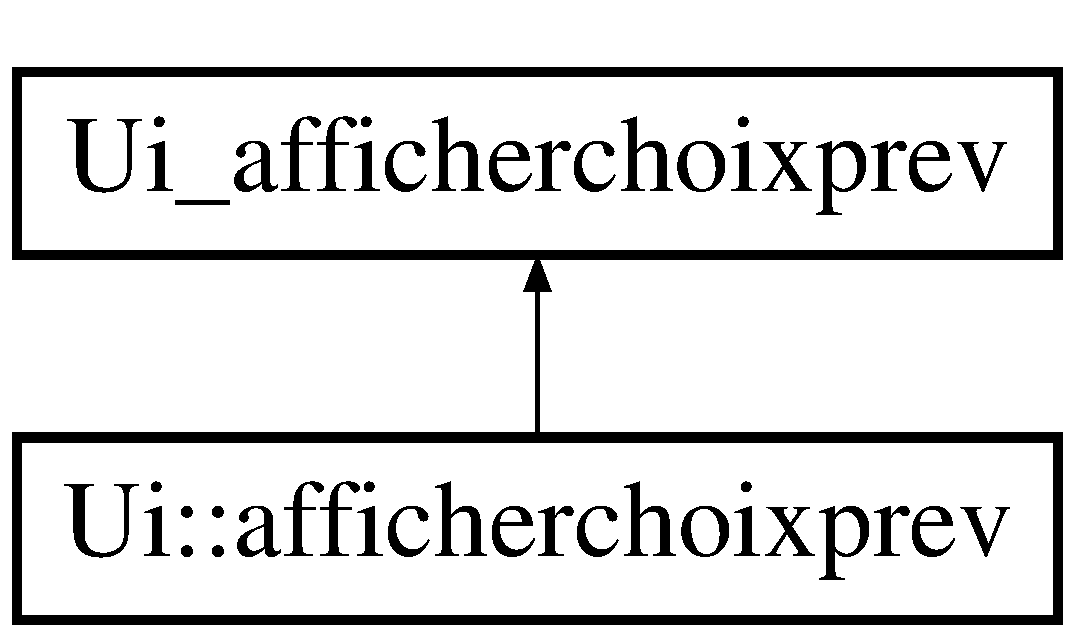
\includegraphics[height=2.000000cm]{class_ui_1_1afficherchoixprev}
\end{center}
\end{figure}
\subsection*{Membres hérités additionnels}


La documentation de cette classe a été générée à partir du fichier suivant \+:\begin{DoxyCompactItemize}
\item 
ui\+\_\+afficherchoixprev.\+h\end{DoxyCompactItemize}

\hypertarget{classafficherchoixprev}{\section{Référence de la classe afficherchoixprev}
\label{classafficherchoixprev}\index{afficherchoixprev@{afficherchoixprev}}
}
Graphe d'héritage de afficherchoixprev\+:\begin{figure}[H]
\begin{center}
\leavevmode
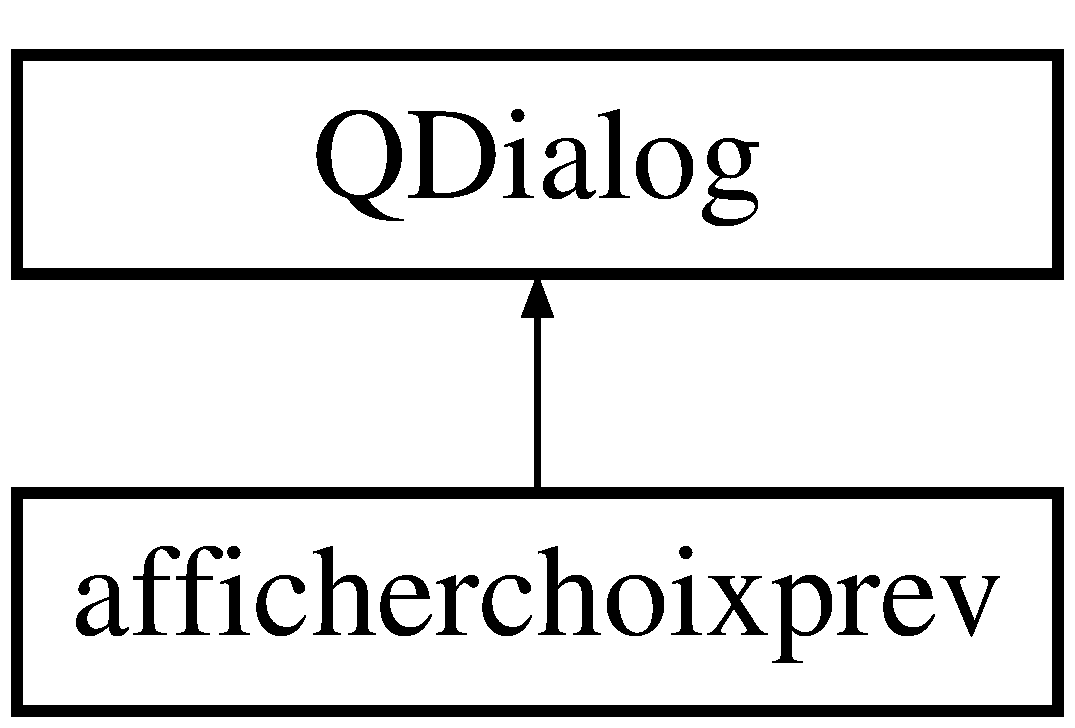
\includegraphics[height=2.000000cm]{classafficherchoixprev}
\end{center}
\end{figure}
\subsection*{Fonctions membres publiques}
\begin{DoxyCompactItemize}
\item 
\hypertarget{classafficherchoixprev_a02f77cdfa3f0a2a26e92785318974685}{{\bfseries afficherchoixprev} (Q\+Dialog $\ast$parent=0)}\label{classafficherchoixprev_a02f77cdfa3f0a2a26e92785318974685}

\item 
\hypertarget{classafficherchoixprev_af9d7d017f015f7f9931b0cc1bcd6625b}{void {\bfseries ajoutprev} (Mapsugg\+\_\+\+U\+V mapsuggestion)}\label{classafficherchoixprev_af9d7d017f015f7f9931b0cc1bcd6625b}

\end{DoxyCompactItemize}


La documentation de cette classe a été générée à partir des fichiers suivants \+:\begin{DoxyCompactItemize}
\item 
afficherchoixprev.\+h\item 
afficherchoixprev.\+cpp\end{DoxyCompactItemize}

\hypertarget{class_branches}{\section{Référence de la classe Branches}
\label{class_branches}\index{Branches@{Branches}}
}
Graphe d'héritage de Branches\+:\begin{figure}[H]
\begin{center}
\leavevmode
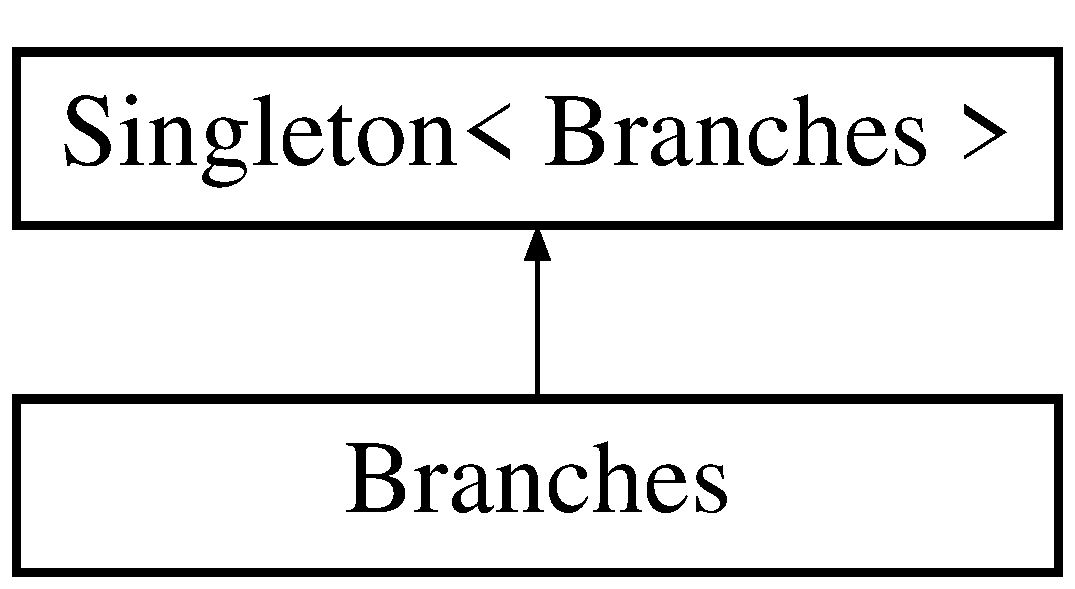
\includegraphics[height=2.000000cm]{class_branches}
\end{center}
\end{figure}
\subsection*{Fonctions membres publiques}
\begin{DoxyCompactItemize}
\item 
\hypertarget{class_branches_a9e69f2be479a387cd4f53bf3816f42b3}{Q\+String\+List \& {\bfseries get\+Liste\+\_\+branches} ()}\label{class_branches_a9e69f2be479a387cd4f53bf3816f42b3}

\item 
\hypertarget{class_branches_a49fdbe17f643c7e4259e9e1fdd6bcb29}{Q\+String\+List {\bfseries get\+Branches\+From\+Cursus} (const Q\+String \&cursus)}\label{class_branches_a49fdbe17f643c7e4259e9e1fdd6bcb29}

\item 
\hypertarget{class_branches_ac262115f02d31604b4449deea5cd3ac9}{void {\bfseries push\+\_\+back} (Q\+String item)}\label{class_branches_ac262115f02d31604b4449deea5cd3ac9}

\item 
\hypertarget{class_branches_accdfc3897bb17a159e0eddb954383bf4}{void {\bfseries remove\+At} (int row)}\label{class_branches_accdfc3897bb17a159e0eddb954383bf4}

\item 
\hypertarget{class_branches_a6b80b177bb7b371cb3f1a5093ea6c034}{void {\bfseries set\+Liste\+\_\+branches} (Q\+String\+List \&l)}\label{class_branches_a6b80b177bb7b371cb3f1a5093ea6c034}

\end{DoxyCompactItemize}
\subsection*{Amis}
\begin{DoxyCompactItemize}
\item 
\hypertarget{class_branches_a742d1f66e36ac560e68852b7180bf5e5}{class {\bfseries Singleton$<$ Branches $>$}}\label{class_branches_a742d1f66e36ac560e68852b7180bf5e5}

\end{DoxyCompactItemize}
\subsection*{Membres hérités additionnels}


La documentation de cette classe a été générée à partir des fichiers suivants \+:\begin{DoxyCompactItemize}
\item 
branches.\+h\item 
branches.\+cpp\end{DoxyCompactItemize}

\hypertarget{class_categorie}{\section{Référence de la classe Categorie}
\label{class_categorie}\index{Categorie@{Categorie}}
}
Graphe d'héritage de Categorie\+:\begin{figure}[H]
\begin{center}
\leavevmode
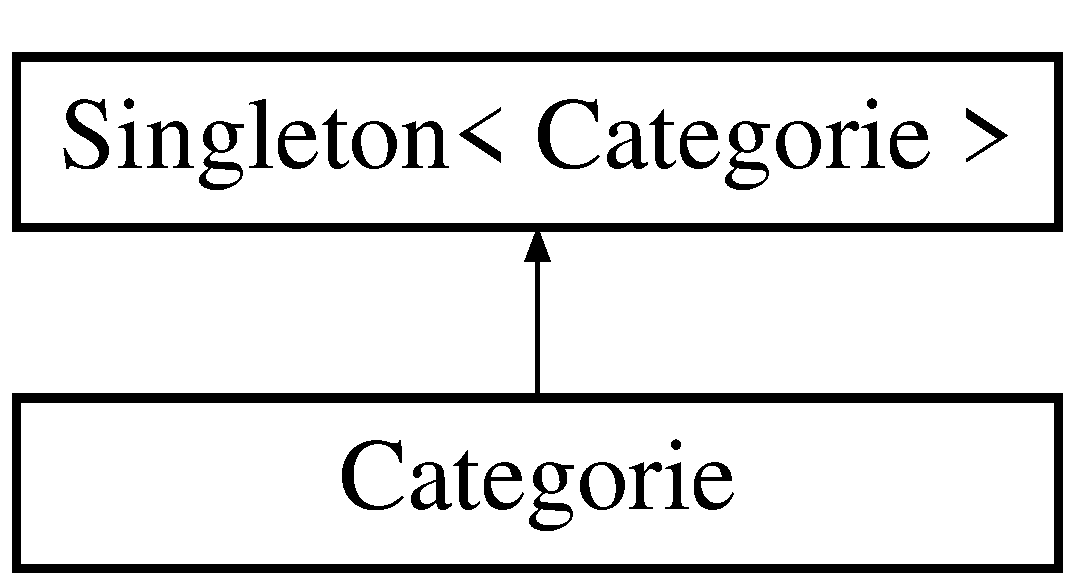
\includegraphics[height=2.000000cm]{class_categorie}
\end{center}
\end{figure}
\subsection*{Fonctions membres publiques}
\begin{DoxyCompactItemize}
\item 
\hypertarget{class_categorie_a1a5b66b96088fd925281e98292850999}{Q\+String\+List \& {\bfseries get\+Liste\+\_\+categories} ()}\label{class_categorie_a1a5b66b96088fd925281e98292850999}

\item 
\hypertarget{class_categorie_aedf4676357581efafda630ae1920f153}{void {\bfseries push\+\_\+back} (Q\+String item)}\label{class_categorie_aedf4676357581efafda630ae1920f153}

\item 
\hypertarget{class_categorie_a2c38ad4e3d79107b16105fb2546f30a8}{void {\bfseries remove\+At} (int row)}\label{class_categorie_a2c38ad4e3d79107b16105fb2546f30a8}

\item 
\hypertarget{class_categorie_ad7c93d27fa0291eab42e72bc7466a3bf}{void {\bfseries set\+Liste\+\_\+categories} (Q\+String\+List \&l)}\label{class_categorie_ad7c93d27fa0291eab42e72bc7466a3bf}

\end{DoxyCompactItemize}
\subsection*{Amis}
\begin{DoxyCompactItemize}
\item 
\hypertarget{class_categorie_a7f9e2dd5a60262d4a4a9dab397a68ed0}{class {\bfseries Singleton$<$ Categorie $>$}}\label{class_categorie_a7f9e2dd5a60262d4a4a9dab397a68ed0}

\end{DoxyCompactItemize}
\subsection*{Membres hérités additionnels}


La documentation de cette classe a été générée à partir des fichiers suivants \+:\begin{DoxyCompactItemize}
\item 
categorie.\+h\item 
categorie.\+cpp\end{DoxyCompactItemize}

\hypertarget{classchoixprevisionnel}{\section{Référence de la classe choixprevisionnel}
\label{classchoixprevisionnel}\index{choixprevisionnel@{choixprevisionnel}}
}
Graphe d'héritage de choixprevisionnel\+:\begin{figure}[H]
\begin{center}
\leavevmode
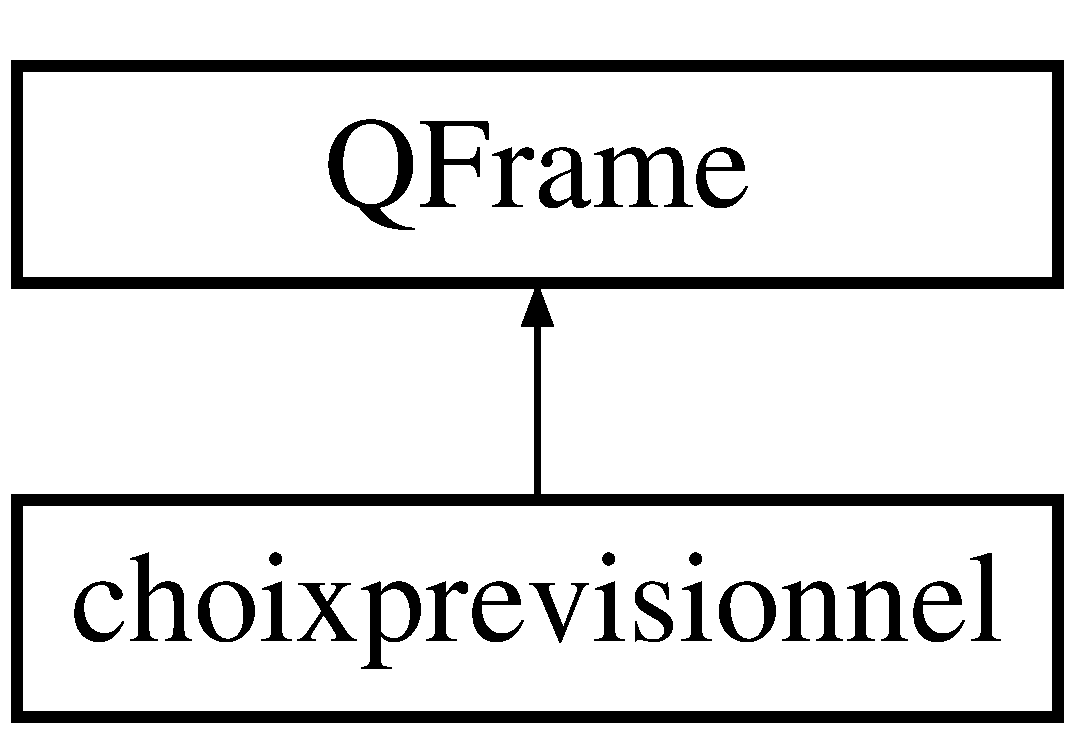
\includegraphics[height=2.000000cm]{classchoixprevisionnel}
\end{center}
\end{figure}
\subsection*{Fonctions membres publiques}
\begin{DoxyCompactItemize}
\item 
\hypertarget{classchoixprevisionnel_ab1e7bdc8754f678ad9146ee35dc65c7c}{{\bfseries choixprevisionnel} (Q\+Widget $\ast$parent=0)}\label{classchoixprevisionnel_ab1e7bdc8754f678ad9146ee35dc65c7c}

\end{DoxyCompactItemize}


La documentation de cette classe a été générée à partir des fichiers suivants \+:\begin{DoxyCompactItemize}
\item 
choixprevisionnel.\+h\item 
choixprevisionnel.\+cpp\end{DoxyCompactItemize}

\hypertarget{class_connexion}{\section{Référence de la classe Connexion}
\label{class_connexion}\index{Connexion@{Connexion}}
}
Graphe d'héritage de Connexion\+:\begin{figure}[H]
\begin{center}
\leavevmode
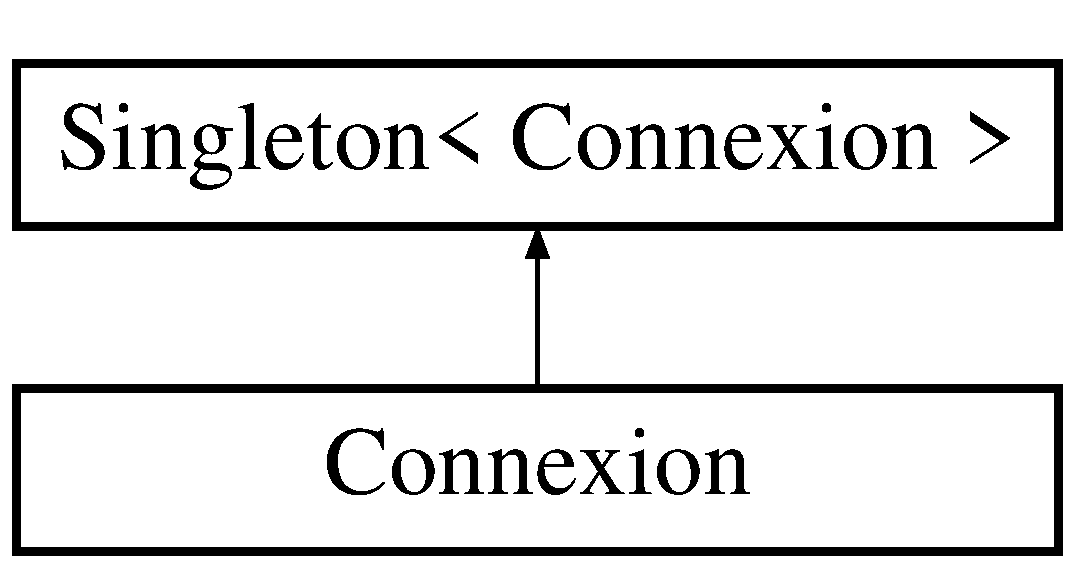
\includegraphics[height=2.000000cm]{class_connexion}
\end{center}
\end{figure}
\subsection*{Fonctions membres publiques}
\begin{DoxyCompactItemize}
\item 
\hypertarget{class_connexion_a2475dca7bbaf306d42b2e78f2f0cf08d}{Q\+String {\bfseries connexion} (Q\+String login, Q\+String mdp)}\label{class_connexion_a2475dca7bbaf306d42b2e78f2f0cf08d}

\item 
\hypertarget{class_connexion_a1df48b898953e64849a8a541be1f7aee}{bool {\bfseries is\+Connected} () const }\label{class_connexion_a1df48b898953e64849a8a541be1f7aee}

\item 
\hypertarget{class_connexion_a711ba0ec90937364ae8ff7067d68ac28}{void {\bfseries set\+Login} (Q\+String l)}\label{class_connexion_a711ba0ec90937364ae8ff7067d68ac28}

\item 
\hypertarget{class_connexion_a3fde06cd178af385b07438aac86c61b3}{void {\bfseries set\+Passwd} (Q\+String p)}\label{class_connexion_a3fde06cd178af385b07438aac86c61b3}

\item 
\hypertarget{class_connexion_a88ef41db366132d1cd48387b4806e03f}{void {\bfseries set\+Nom} (Q\+String n)}\label{class_connexion_a88ef41db366132d1cd48387b4806e03f}

\item 
\hypertarget{class_connexion_a4ec36b38a59d38b1bfee2933a5379d2d}{void {\bfseries set\+Prenom} (Q\+String p)}\label{class_connexion_a4ec36b38a59d38b1bfee2933a5379d2d}

\item 
\hypertarget{class_connexion_a17e79c1d04b1e5d5d18b9ccded6778b3}{void {\bfseries set\+Sexe} (Q\+String s)}\label{class_connexion_a17e79c1d04b1e5d5d18b9ccded6778b3}

\item 
\hypertarget{class_connexion_a0437b302f989a63e5e0fae37b26cbdcd}{void {\bfseries set\+Date\+\_\+naissance} (Q\+String d)}\label{class_connexion_a0437b302f989a63e5e0fae37b26cbdcd}

\item 
\hypertarget{class_connexion_a714db9bc9a522e4778fddad78b30c115}{void {\bfseries set\+Email} (Q\+String e)}\label{class_connexion_a714db9bc9a522e4778fddad78b30c115}

\item 
\hypertarget{class_connexion_a24889880f5ce6cc8b64318882486e7e1}{void {\bfseries set\+Commentaires} (Q\+String c)}\label{class_connexion_a24889880f5ce6cc8b64318882486e7e1}

\item 
\hypertarget{class_connexion_a4a19b40a17e3590b65ea83248291d9f9}{Q\+String {\bfseries get\+Login} () const }\label{class_connexion_a4a19b40a17e3590b65ea83248291d9f9}

\item 
\hypertarget{class_connexion_a559bc5706037b5928eee6c079f83720c}{Q\+String {\bfseries get\+Passwd} () const }\label{class_connexion_a559bc5706037b5928eee6c079f83720c}

\item 
\hypertarget{class_connexion_ab957cd2da042d7ff62e563ad548e0e32}{Q\+String {\bfseries get\+Nom} () const }\label{class_connexion_ab957cd2da042d7ff62e563ad548e0e32}

\item 
\hypertarget{class_connexion_a49af3f021e0034da75fb95dde5610865}{Q\+String {\bfseries get\+Prenom} () const }\label{class_connexion_a49af3f021e0034da75fb95dde5610865}

\item 
\hypertarget{class_connexion_a3da79d1264dbe24afa1b2b3a77d00f36}{Q\+String {\bfseries get\+Sexe} () const }\label{class_connexion_a3da79d1264dbe24afa1b2b3a77d00f36}

\item 
\hypertarget{class_connexion_a0343b541b2770d6545ace11a8bcdad85}{Q\+String {\bfseries get\+Date\+\_\+naissance} () const }\label{class_connexion_a0343b541b2770d6545ace11a8bcdad85}

\item 
\hypertarget{class_connexion_a88f0556be9e142edcce90de4b48c0255}{Q\+String {\bfseries get\+Email} () const }\label{class_connexion_a88f0556be9e142edcce90de4b48c0255}

\item 
\hypertarget{class_connexion_ae84dc007affc87f4d4639b4a018e1d18}{Q\+String {\bfseries get\+Commentaires} () const }\label{class_connexion_ae84dc007affc87f4d4639b4a018e1d18}

\end{DoxyCompactItemize}
\subsection*{Amis}
\begin{DoxyCompactItemize}
\item 
\hypertarget{class_connexion_aa45b32173e97ceffd41065ae6c80a029}{class {\bfseries Singleton$<$ Connexion $>$}}\label{class_connexion_aa45b32173e97ceffd41065ae6c80a029}

\end{DoxyCompactItemize}
\subsection*{Membres hérités additionnels}


La documentation de cette classe a été générée à partir des fichiers suivants \+:\begin{DoxyCompactItemize}
\item 
connexion.\+h\item 
connexion.\+cpp\end{DoxyCompactItemize}

\hypertarget{class_cursus}{\section{Référence de la classe Cursus}
\label{class_cursus}\index{Cursus@{Cursus}}
}
Graphe d'héritage de Cursus\+:\begin{figure}[H]
\begin{center}
\leavevmode
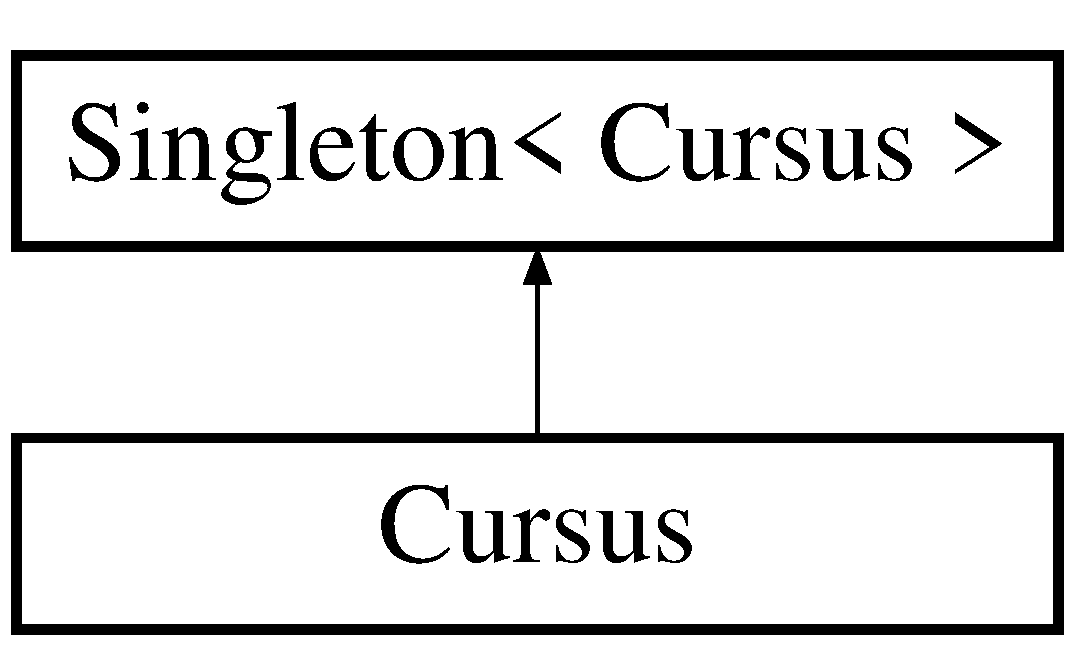
\includegraphics[height=2.000000cm]{class_cursus}
\end{center}
\end{figure}
\subsection*{Fonctions membres publiques}
\begin{DoxyCompactItemize}
\item 
\hypertarget{class_cursus_ab66bff51a6422dcb2342fe94fd8062f5}{Q\+String\+List \& {\bfseries get\+Liste\+\_\+cursus} ()}\label{class_cursus_ab66bff51a6422dcb2342fe94fd8062f5}

\item 
\hypertarget{class_cursus_ae64961c683e50fd22deb9a9242094407}{void {\bfseries push\+\_\+back} (Q\+String item)}\label{class_cursus_ae64961c683e50fd22deb9a9242094407}

\item 
\hypertarget{class_cursus_a50e8abb051af0a937fec5a95fd598ba7}{void {\bfseries remove\+At} (int row)}\label{class_cursus_a50e8abb051af0a937fec5a95fd598ba7}

\item 
\hypertarget{class_cursus_a938c8831a597dbeef047958ed614c0fb}{void {\bfseries set\+Liste\+\_\+cursus} (Q\+String\+List \&l)}\label{class_cursus_a938c8831a597dbeef047958ed614c0fb}

\end{DoxyCompactItemize}
\subsection*{Amis}
\begin{DoxyCompactItemize}
\item 
\hypertarget{class_cursus_a39488d3df381e1f57721cebe5054e4d3}{class {\bfseries Singleton$<$ Cursus $>$}}\label{class_cursus_a39488d3df381e1f57721cebe5054e4d3}

\end{DoxyCompactItemize}
\subsection*{Membres hérités additionnels}


La documentation de cette classe a été générée à partir des fichiers suivants \+:\begin{DoxyCompactItemize}
\item 
cursus.\+h\item 
cursus.\+cpp\end{DoxyCompactItemize}

\hypertarget{classdbmanager}{\section{Référence de la classe dbmanager}
\label{classdbmanager}\index{dbmanager@{dbmanager}}
}
Graphe d'héritage de dbmanager\+:\begin{figure}[H]
\begin{center}
\leavevmode
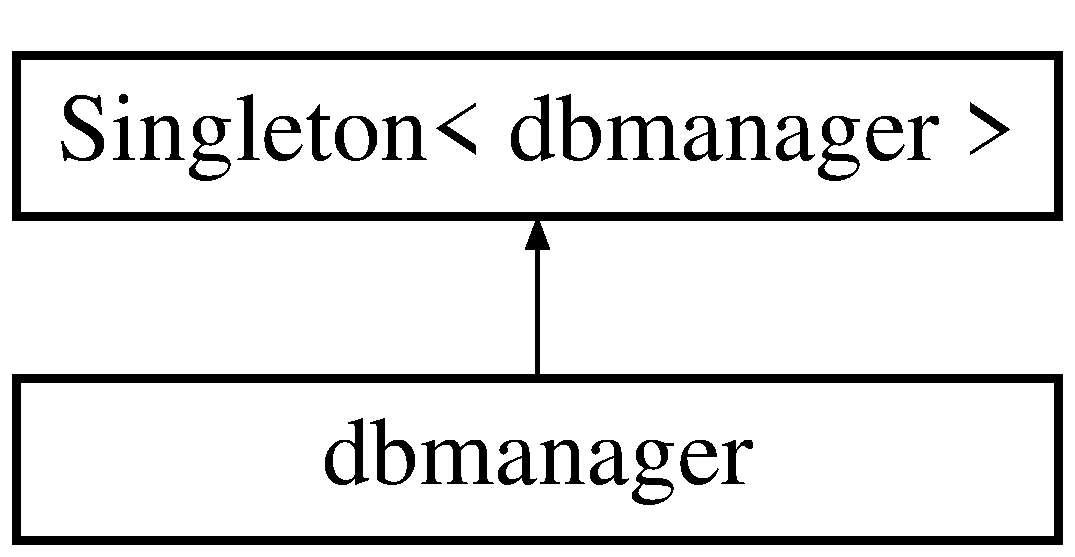
\includegraphics[height=2.000000cm]{classdbmanager}
\end{center}
\end{figure}
\subsection*{Fonctions membres publiques}
\begin{DoxyCompactItemize}
\item 
\hypertarget{classdbmanager_ad0554aaf4742853ae68f2ce9c73e0f03}{void {\bfseries dbinitialise} (Q\+String dbtype, Q\+String dbhost, Q\+String dbuser, Q\+String dbpasswd, Q\+String dbname)}\label{classdbmanager_ad0554aaf4742853ae68f2ce9c73e0f03}

\item 
\hypertarget{classdbmanager_a6896e1989994ffb1dfbfdfb8bf91cb65}{void {\bfseries dbinitialise} (Q\+String dbtype, Q\+String dbname)}\label{classdbmanager_a6896e1989994ffb1dfbfdfb8bf91cb65}

\item 
\hypertarget{classdbmanager_ab6e8b56be8e6286dbe92406a969e2d0f}{void {\bfseries dbclose} ()}\label{classdbmanager_ab6e8b56be8e6286dbe92406a969e2d0f}

\item 
\hypertarget{classdbmanager_a74263e13f442c48179e7339370ad0df6}{Q\+Sql\+Database {\bfseries get\+Value} ()}\label{classdbmanager_a74263e13f442c48179e7339370ad0df6}

\item 
\hypertarget{classdbmanager_aadd93a1f6de3210ba3ff63fd1a769d65}{Q\+Sql\+Query {\bfseries execute} (Q\+String marequete)}\label{classdbmanager_aadd93a1f6de3210ba3ff63fd1a769d65}

\item 
\hypertarget{classdbmanager_a31cce1e1ece40bbeec5ee1ddda85614b}{Q\+String\+List {\bfseries get\+Colonne} (Q\+String requete)}\label{classdbmanager_a31cce1e1ece40bbeec5ee1ddda85614b}

\end{DoxyCompactItemize}
\subsection*{Amis}
\begin{DoxyCompactItemize}
\item 
\hypertarget{classdbmanager_af8de2880270e7199a9802839897b9c7d}{class {\bfseries Singleton$<$ dbmanager $>$}}\label{classdbmanager_af8de2880270e7199a9802839897b9c7d}

\end{DoxyCompactItemize}
\subsection*{Membres hérités additionnels}


La documentation de cette classe a été générée à partir des fichiers suivants \+:\begin{DoxyCompactItemize}
\item 
dbmanager.\+h\item 
dbmanager.\+cpp\end{DoxyCompactItemize}

\hypertarget{class_ui_1_1detailuv}{\section{Référence de la classe Ui\+:\+:detailuv}
\label{class_ui_1_1detailuv}\index{Ui\+::detailuv@{Ui\+::detailuv}}
}
Graphe d'héritage de Ui\+:\+:detailuv\+:\begin{figure}[H]
\begin{center}
\leavevmode
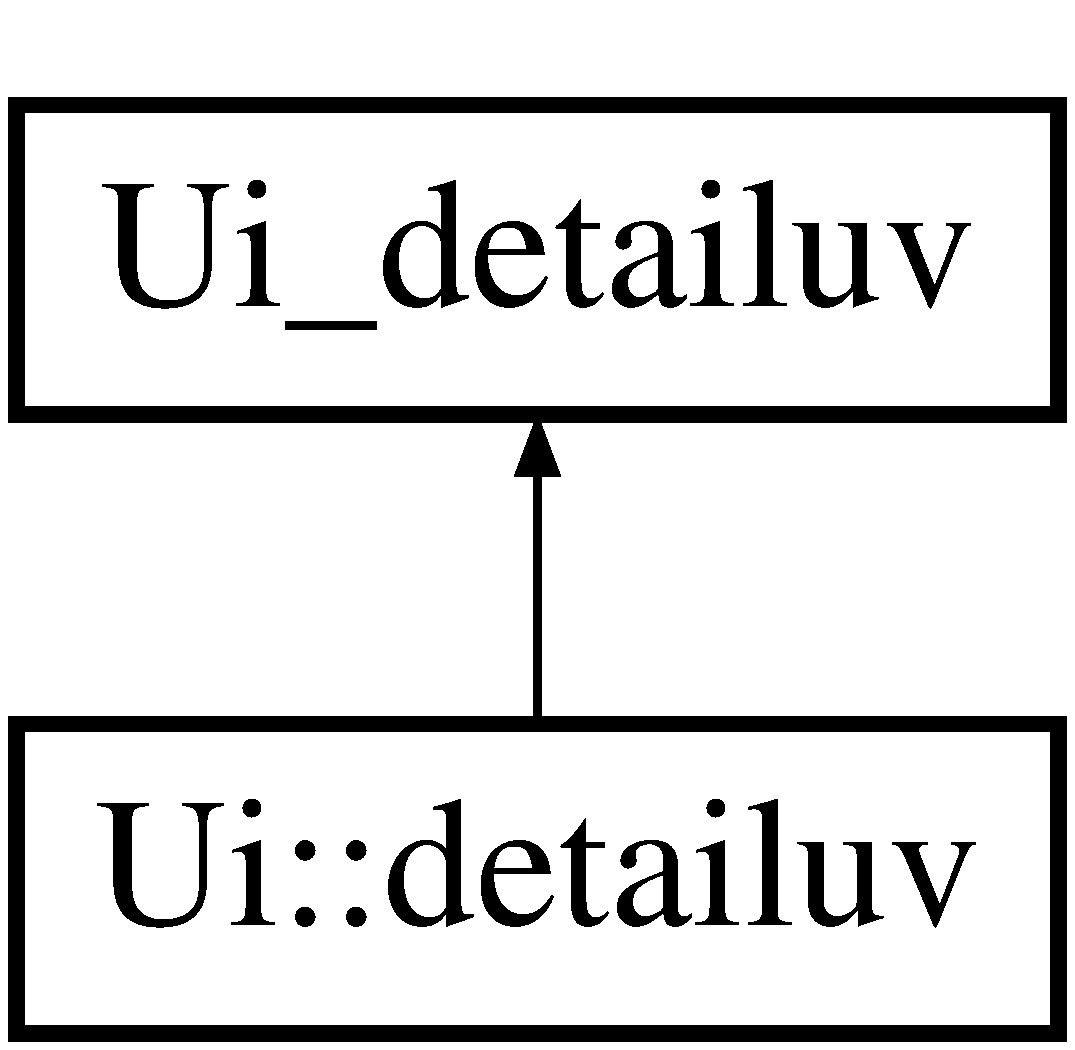
\includegraphics[height=2.000000cm]{class_ui_1_1detailuv}
\end{center}
\end{figure}
\subsection*{Membres hérités additionnels}


La documentation de cette classe a été générée à partir du fichier suivant \+:\begin{DoxyCompactItemize}
\item 
ui\+\_\+detailuv.\+h\end{DoxyCompactItemize}

\hypertarget{classdetailuv}{\section{Référence de la classe detailuv}
\label{classdetailuv}\index{detailuv@{detailuv}}
}
Graphe d'héritage de detailuv\+:\begin{figure}[H]
\begin{center}
\leavevmode
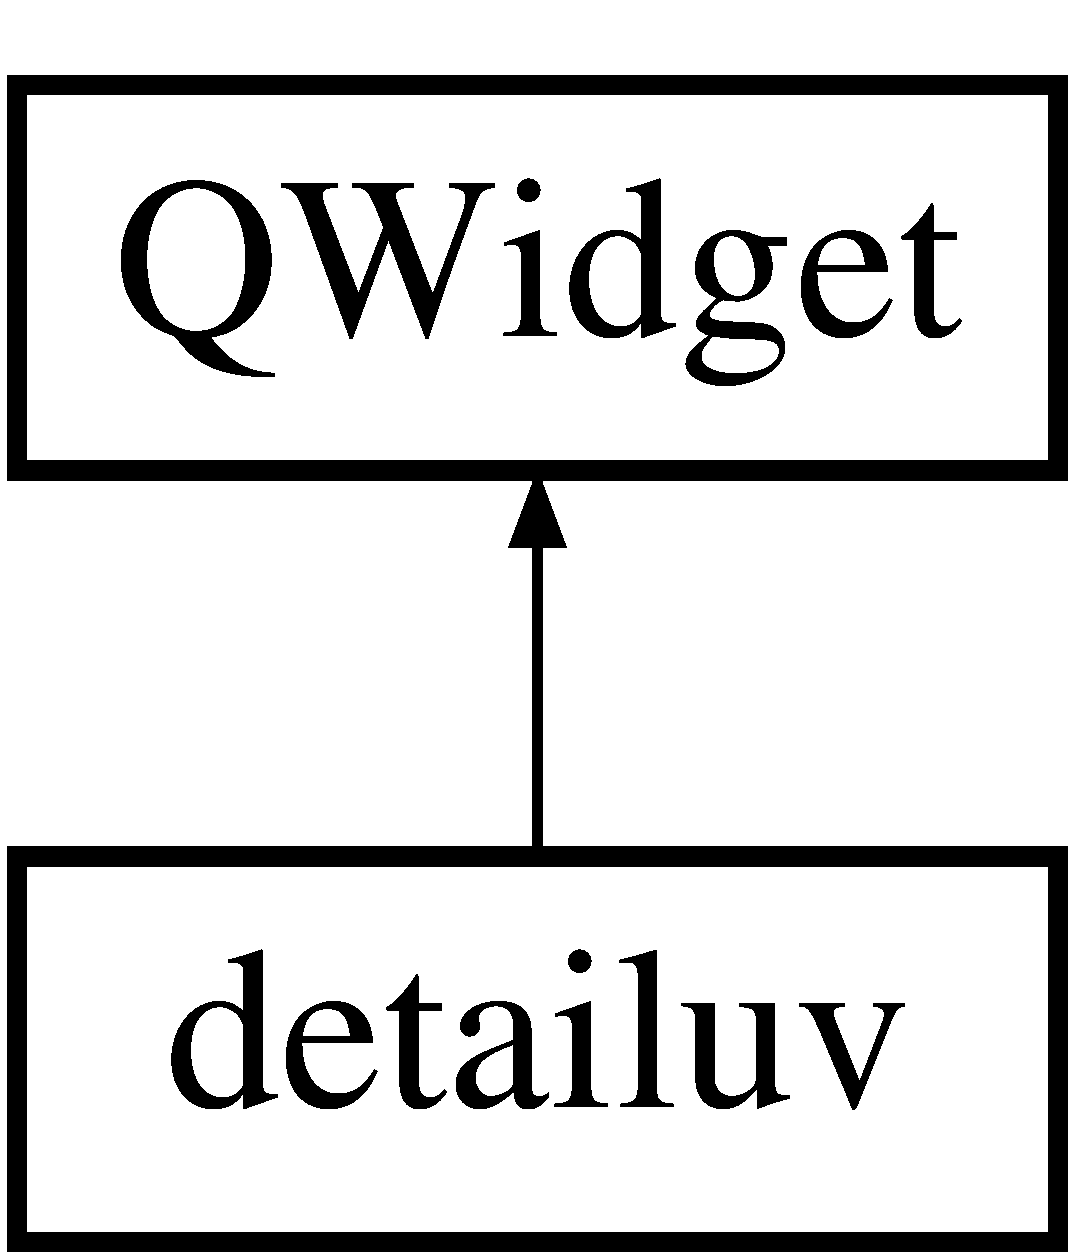
\includegraphics[height=2.000000cm]{classdetailuv}
\end{center}
\end{figure}
\subsection*{Fonctions membres publiques}
\begin{DoxyCompactItemize}
\item 
\hypertarget{classdetailuv_a043d04e316874b6403266262ce295126}{{\bfseries detailuv} (Q\+Widget $\ast$parent=0)}\label{classdetailuv_a043d04e316874b6403266262ce295126}

\end{DoxyCompactItemize}


La documentation de cette classe a été générée à partir des fichiers suivants \+:\begin{DoxyCompactItemize}
\item 
detailuv.\+h\item 
detailuv.\+cpp\end{DoxyCompactItemize}

\hypertarget{class_disponibilites}{\section{Référence de la classe Disponibilites}
\label{class_disponibilites}\index{Disponibilites@{Disponibilites}}
}
Graphe d'héritage de Disponibilites\+:\begin{figure}[H]
\begin{center}
\leavevmode
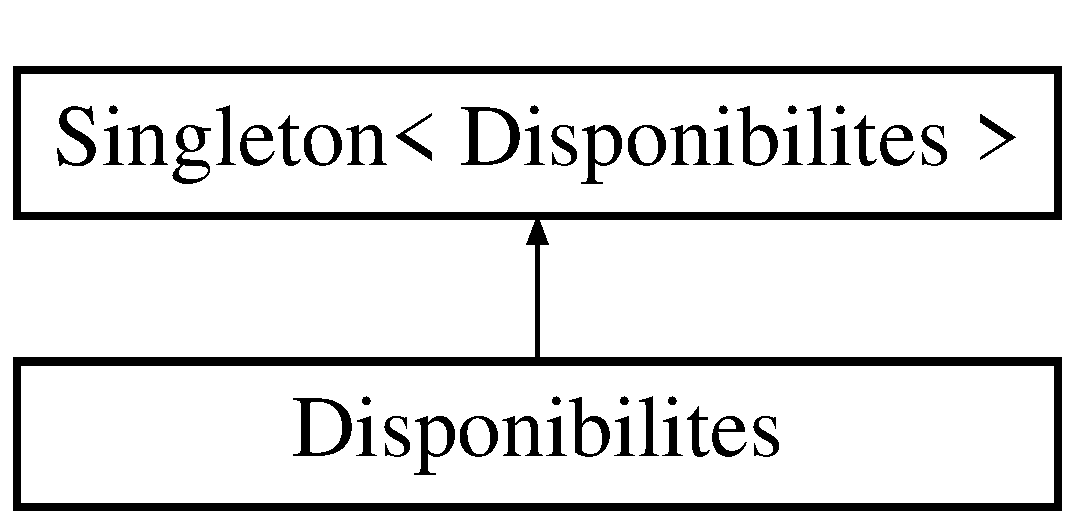
\includegraphics[height=2.000000cm]{class_disponibilites}
\end{center}
\end{figure}
\subsection*{Fonctions membres publiques}
\begin{DoxyCompactItemize}
\item 
\hypertarget{class_disponibilites_a7a0c84d0b8731cbd55209ed928d1799f}{Q\+String\+List \& {\bfseries get\+Liste\+\_\+dispos} ()}\label{class_disponibilites_a7a0c84d0b8731cbd55209ed928d1799f}

\item 
\hypertarget{class_disponibilites_a7c9c7950057ae4c31eeb589a35bea28a}{void {\bfseries push\+\_\+back} (Q\+String item)}\label{class_disponibilites_a7c9c7950057ae4c31eeb589a35bea28a}

\item 
\hypertarget{class_disponibilites_aa109462728f928dee2a2f96324ae8b85}{void {\bfseries remove\+At} (int row)}\label{class_disponibilites_aa109462728f928dee2a2f96324ae8b85}

\item 
\hypertarget{class_disponibilites_abbc56d1b6926971fd3f6dc626bcd1c08}{void {\bfseries set\+Liste\+\_\+dispos} (Q\+String\+List \&l)}\label{class_disponibilites_abbc56d1b6926971fd3f6dc626bcd1c08}

\end{DoxyCompactItemize}
\subsection*{Amis}
\begin{DoxyCompactItemize}
\item 
\hypertarget{class_disponibilites_aaf5bfd019b36b22eec3a2add26a4bab6}{class {\bfseries Singleton$<$ Disponibilites $>$}}\label{class_disponibilites_aaf5bfd019b36b22eec3a2add26a4bab6}

\end{DoxyCompactItemize}
\subsection*{Membres hérités additionnels}


La documentation de cette classe a été générée à partir des fichiers suivants \+:\begin{DoxyCompactItemize}
\item 
disponibilites.\+h\item 
disponibilites.\+cpp\end{DoxyCompactItemize}

\hypertarget{class_dossier}{\section{Référence de la classe Dossier}
\label{class_dossier}\index{Dossier@{Dossier}}
}


La documentation de cette classe a été générée à partir du fichier suivant \+:\begin{DoxyCompactItemize}
\item 
uvmanager.\+h\end{DoxyCompactItemize}

\hypertarget{class_etudiants}{\section{Référence de la classe Etudiants}
\label{class_etudiants}\index{Etudiants@{Etudiants}}
}
Graphe d'héritage de Etudiants\+:\begin{figure}[H]
\begin{center}
\leavevmode
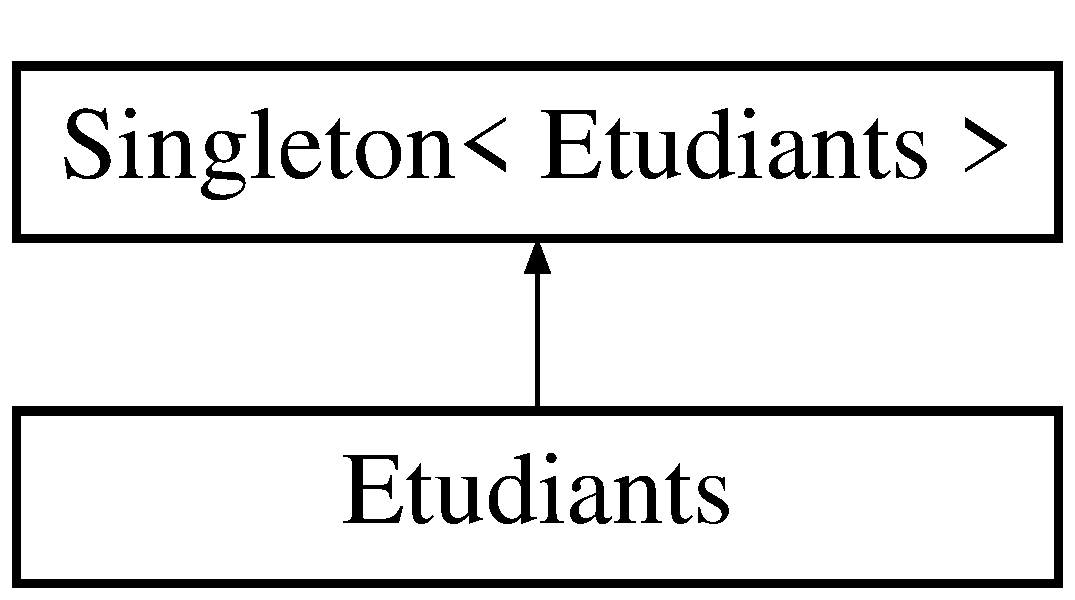
\includegraphics[height=2.000000cm]{class_etudiants}
\end{center}
\end{figure}
\subsection*{Fonctions membres publiques}
\begin{DoxyCompactItemize}
\item 
\hypertarget{class_etudiants_a872d4a8dd0354322e067a67d0c3b67a1}{Q\+String\+List \& {\bfseries get\+Liste\+\_\+etudiants} ()}\label{class_etudiants_a872d4a8dd0354322e067a67d0c3b67a1}

\item 
\hypertarget{class_etudiants_aad7ffc509ea5ab7c0e4627bf5da1081d}{void {\bfseries push\+\_\+back} (Q\+String item)}\label{class_etudiants_aad7ffc509ea5ab7c0e4627bf5da1081d}

\item 
\hypertarget{class_etudiants_adfc202eb11688821712cf773365ac035}{void {\bfseries remove\+At} (int row)}\label{class_etudiants_adfc202eb11688821712cf773365ac035}

\item 
\hypertarget{class_etudiants_afb5396339b61c6a026a1e9b87a1aecf6}{void {\bfseries set\+Liste\+\_\+etudiants} (Q\+String\+List \&l)}\label{class_etudiants_afb5396339b61c6a026a1e9b87a1aecf6}

\end{DoxyCompactItemize}
\subsection*{Amis}
\begin{DoxyCompactItemize}
\item 
\hypertarget{class_etudiants_a6956ca5228b95aa3879716fff6302476}{class {\bfseries Singleton$<$ Etudiants $>$}}\label{class_etudiants_a6956ca5228b95aa3879716fff6302476}

\end{DoxyCompactItemize}
\subsection*{Membres hérités additionnels}


La documentation de cette classe a été générée à partir des fichiers suivants \+:\begin{DoxyCompactItemize}
\item 
etudiants.\+h\item 
etudiants.\+cpp\end{DoxyCompactItemize}

\hypertarget{class_ui_1_1fenetreplus}{\section{Référence de la classe Ui\+:\+:fenetreplus}
\label{class_ui_1_1fenetreplus}\index{Ui\+::fenetreplus@{Ui\+::fenetreplus}}
}
Graphe d'héritage de Ui\+:\+:fenetreplus\+:\begin{figure}[H]
\begin{center}
\leavevmode
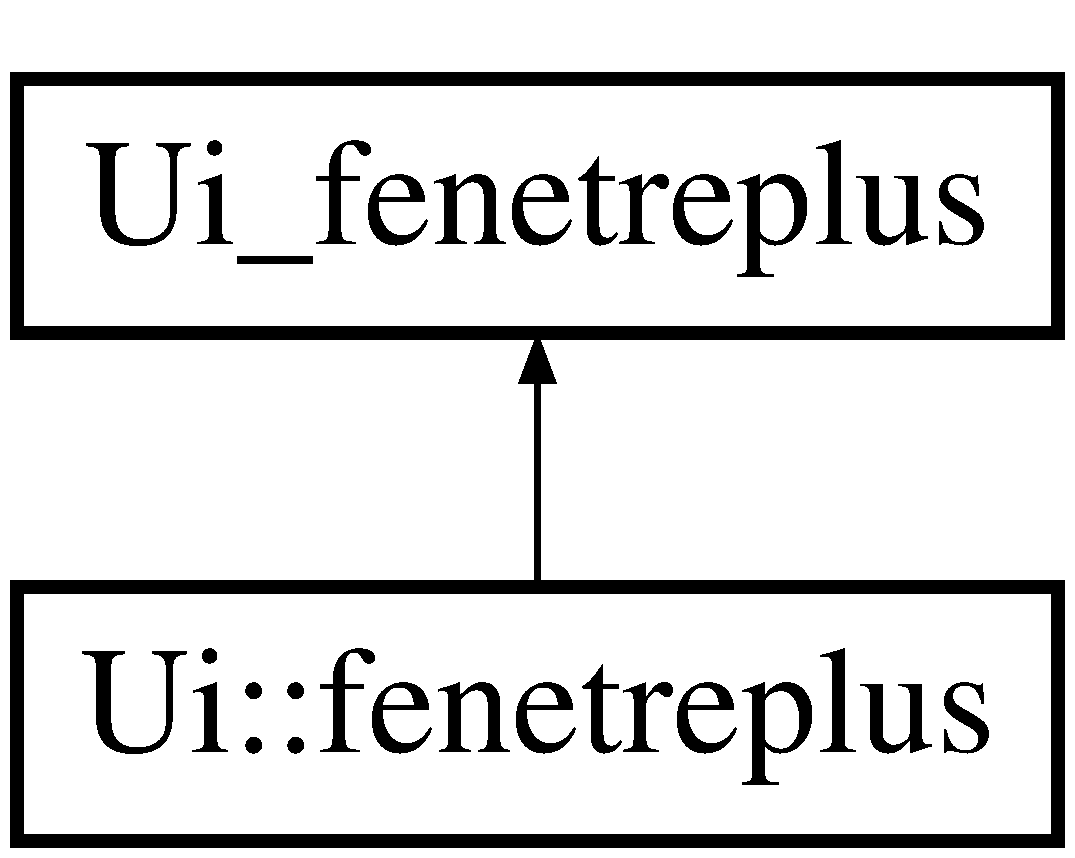
\includegraphics[height=2.000000cm]{class_ui_1_1fenetreplus}
\end{center}
\end{figure}
\subsection*{Membres hérités additionnels}


La documentation de cette classe a été générée à partir du fichier suivant \+:\begin{DoxyCompactItemize}
\item 
ui\+\_\+fenetreplus.\+h\end{DoxyCompactItemize}

\hypertarget{classfenetreplus}{\section{Référence de la classe fenetreplus}
\label{classfenetreplus}\index{fenetreplus@{fenetreplus}}
}
Graphe d'héritage de fenetreplus\+:\begin{figure}[H]
\begin{center}
\leavevmode
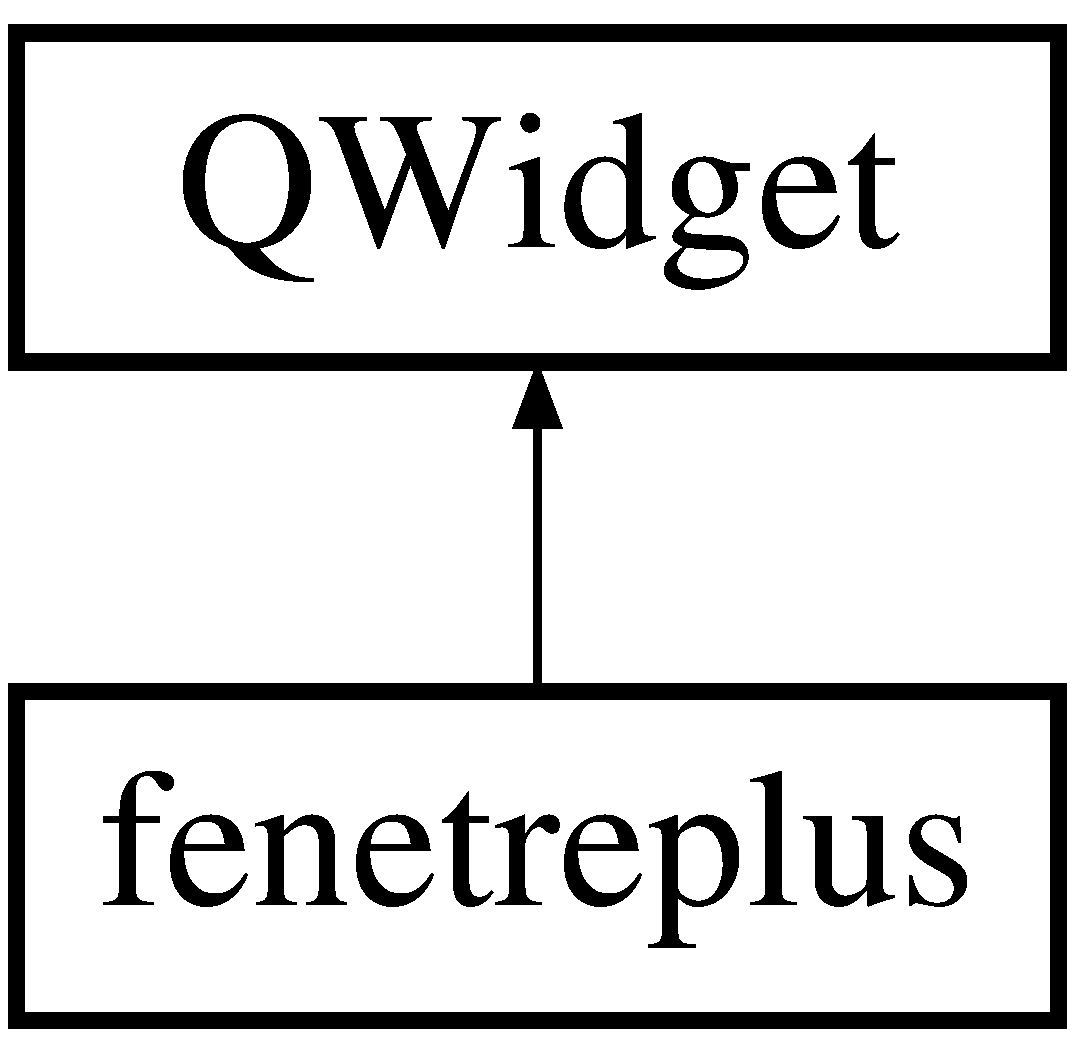
\includegraphics[height=2.000000cm]{classfenetreplus}
\end{center}
\end{figure}
\subsection*{Connecteurs publics}
\begin{DoxyCompactItemize}
\item 
\hypertarget{classfenetreplus_a6fe7c527b188f24c973b901005132c86}{void {\bfseries rendre\+Visible} ()}\label{classfenetreplus_a6fe7c527b188f24c973b901005132c86}

\item 
\hypertarget{classfenetreplus_a6020068711d957c8a9d6918de1380395}{void {\bfseries changer\+Position} ()}\label{classfenetreplus_a6020068711d957c8a9d6918de1380395}

\end{DoxyCompactItemize}
\subsection*{Fonctions membres publiques}
\begin{DoxyCompactItemize}
\item 
\hypertarget{classfenetreplus_aeda6edd6e107593519deeda14e9e16b2}{{\bfseries fenetreplus} (Q\+Widget $\ast$parent=0)}\label{classfenetreplus_aeda6edd6e107593519deeda14e9e16b2}

\end{DoxyCompactItemize}


La documentation de cette classe a été générée à partir des fichiers suivants \+:\begin{DoxyCompactItemize}
\item 
fenetreplus.\+h\item 
fenetreplus.\+cpp\end{DoxyCompactItemize}

\hypertarget{class_fen_xC3_xAAtre}{\section{Référence de la classe Fenêtre}
\label{class_fen_xC3_xAAtre}\index{Fenêtre@{Fenêtre}}
}


\subsection{Description détaillée}
l'appliacation. Elle permet de se connecter mais également de consulter la liste des \hyperlink{class_u_v}{U\+V} en triant par cursus et par branche 

La documentation de cette classe a été générée à partir du fichier suivant \+:\begin{DoxyCompactItemize}
\item 
\hyperlink{accueil_8h}{accueil.\+h}\end{DoxyCompactItemize}

\hypertarget{class_filieres}{\section{Référence de la classe Filieres}
\label{class_filieres}\index{Filieres@{Filieres}}
}
Graphe d'héritage de Filieres\+:\begin{figure}[H]
\begin{center}
\leavevmode
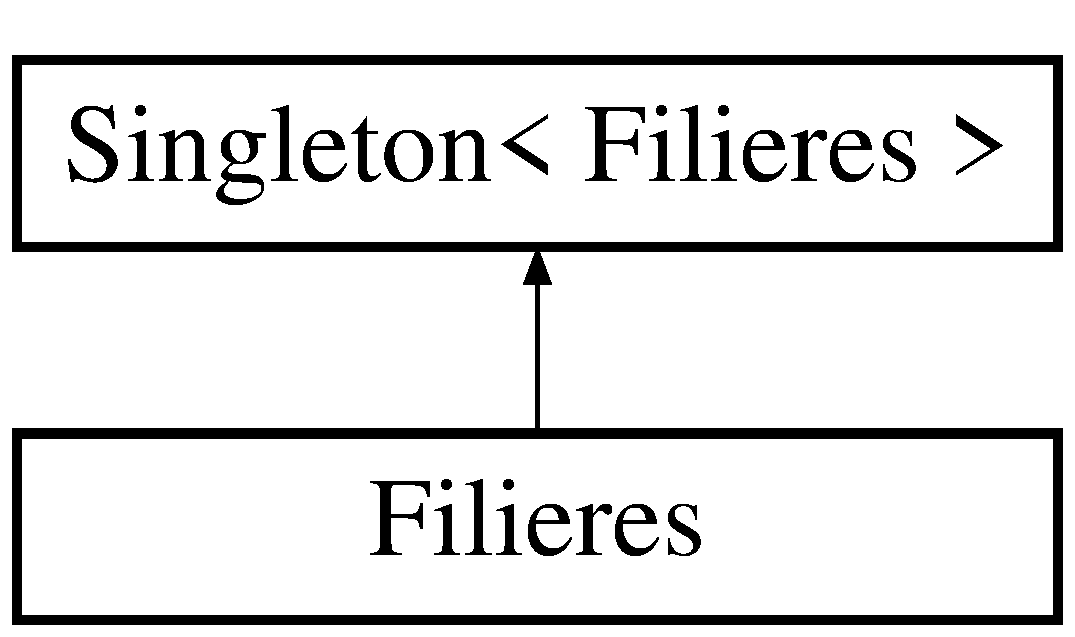
\includegraphics[height=2.000000cm]{class_filieres}
\end{center}
\end{figure}
\subsection*{Fonctions membres publiques}
\begin{DoxyCompactItemize}
\item 
\hypertarget{class_filieres_a2f0f1b73e40690a9350b288f9494b7a8}{Q\+String\+List \& {\bfseries get\+Liste\+\_\+filieres} ()}\label{class_filieres_a2f0f1b73e40690a9350b288f9494b7a8}

\item 
\hypertarget{class_filieres_ac9bf3413a5759e42dc3dc90087185888}{Q\+String\+List {\bfseries get\+Filieres\+From\+Branche} (const Q\+String \&branche)}\label{class_filieres_ac9bf3413a5759e42dc3dc90087185888}

\item 
\hypertarget{class_filieres_ae1ac69e61f3a735b69d07ee1edd3351b}{void {\bfseries push\+\_\+back} (Q\+String item)}\label{class_filieres_ae1ac69e61f3a735b69d07ee1edd3351b}

\item 
\hypertarget{class_filieres_ae630a91b289fd80c964ef8b55c0e560c}{void {\bfseries remove\+At} (int row)}\label{class_filieres_ae630a91b289fd80c964ef8b55c0e560c}

\item 
\hypertarget{class_filieres_af2e5fc56a24633d51c22a9b6b5c9b9fd}{void {\bfseries set\+Liste\+\_\+cursus} (Q\+String\+List \&l)}\label{class_filieres_af2e5fc56a24633d51c22a9b6b5c9b9fd}

\end{DoxyCompactItemize}
\subsection*{Amis}
\begin{DoxyCompactItemize}
\item 
\hypertarget{class_filieres_ac878913a6b3e427b3fd78e64c79c1d42}{class {\bfseries Singleton$<$ Filieres $>$}}\label{class_filieres_ac878913a6b3e427b3fd78e64c79c1d42}

\end{DoxyCompactItemize}
\subsection*{Membres hérités additionnels}


La documentation de cette classe a été générée à partir des fichiers suivants \+:\begin{DoxyCompactItemize}
\item 
filieres.\+h\item 
filieres.\+cpp\end{DoxyCompactItemize}

\hypertarget{class_u_v_manager_1_1_filter_iterator}{\section{Référence de la classe U\+V\+Manager\+:\+:Filter\+Iterator}
\label{class_u_v_manager_1_1_filter_iterator}\index{U\+V\+Manager\+::\+Filter\+Iterator@{U\+V\+Manager\+::\+Filter\+Iterator}}
}
\subsection*{Fonctions membres publiques}
\begin{DoxyCompactItemize}
\item 
\hypertarget{class_u_v_manager_1_1_filter_iterator_a30e4c79f7734cd2b526aed31c437fe47}{bool {\bfseries is\+Done} () const }\label{class_u_v_manager_1_1_filter_iterator_a30e4c79f7734cd2b526aed31c437fe47}

\item 
\hypertarget{class_u_v_manager_1_1_filter_iterator_a60c822de494b70f0837a8c3e241dd3e6}{void {\bfseries next} ()}\label{class_u_v_manager_1_1_filter_iterator_a60c822de494b70f0837a8c3e241dd3e6}

\item 
\hypertarget{class_u_v_manager_1_1_filter_iterator_a1b8f963bba647ce40061ee672e94d6e2}{\hyperlink{class_u_v}{U\+V} \& {\bfseries current} () const }\label{class_u_v_manager_1_1_filter_iterator_a1b8f963bba647ce40061ee672e94d6e2}

\end{DoxyCompactItemize}
\subsection*{Amis}
\begin{DoxyCompactItemize}
\item 
\hypertarget{class_u_v_manager_1_1_filter_iterator_a335ec2026467669b89518b0c67372f3b}{class {\bfseries U\+V\+Manager}}\label{class_u_v_manager_1_1_filter_iterator_a335ec2026467669b89518b0c67372f3b}

\end{DoxyCompactItemize}


La documentation de cette classe a été générée à partir du fichier suivant \+:\begin{DoxyCompactItemize}
\item 
uvmanager.\+h\end{DoxyCompactItemize}

\hypertarget{class_formation}{\section{Référence de la classe Formation}
\label{class_formation}\index{Formation@{Formation}}
}


La documentation de cette classe a été générée à partir du fichier suivant \+:\begin{DoxyCompactItemize}
\item 
uvmanager.\+h\end{DoxyCompactItemize}

\hypertarget{classformulaire}{\section{Référence du modèle de la classe formulaire$<$ T $>$}
\label{classformulaire}\index{formulaire$<$ T $>$@{formulaire$<$ T $>$}}
}
\subsection*{Fonctions membres publiques statiques}
\begin{DoxyCompactItemize}
\item 
\hypertarget{classformulaire_a8d867d6ad49ef76d6ea867c629e4e11b}{static bool {\bfseries verif\+\_\+text} (const T \&txt, const Q\+String \&nomchamp)}\label{classformulaire_a8d867d6ad49ef76d6ea867c629e4e11b}

\item 
\hypertarget{classformulaire_a3b3eb187d90aaa43c0d0850f09446819}{static bool {\bfseries verif\+\_\+pass} (const T \&pass1, const T \&pass2=\char`\"{}xxxxx\char`\"{})}\label{classformulaire_a3b3eb187d90aaa43c0d0850f09446819}

\item 
\hypertarget{classformulaire_a88f12bb3ead2326e7574aa737ffba768}{static bool {\bfseries verif\+\_\+email} (const T \&mail, const Q\+String \&nomchamp)}\label{classformulaire_a88f12bb3ead2326e7574aa737ffba768}

\end{DoxyCompactItemize}
\subsection*{Attributs protégés}
\begin{DoxyCompactItemize}
\item 
\hypertarget{classformulaire_a9a01a0d127eeaf33e9bd14a74c6ceeeb}{unsigned int {\bfseries nb\+Elem}}\label{classformulaire_a9a01a0d127eeaf33e9bd14a74c6ceeeb}

\end{DoxyCompactItemize}


La documentation de cette classe a été générée à partir du fichier suivant \+:\begin{DoxyCompactItemize}
\item 
formulaire.\+h\end{DoxyCompactItemize}

\hypertarget{class_formulaire_exception}{\section{Référence de la classe Formulaire\+Exception}
\label{class_formulaire_exception}\index{Formulaire\+Exception@{Formulaire\+Exception}}
}
Graphe d'héritage de Formulaire\+Exception\+:\begin{figure}[H]
\begin{center}
\leavevmode
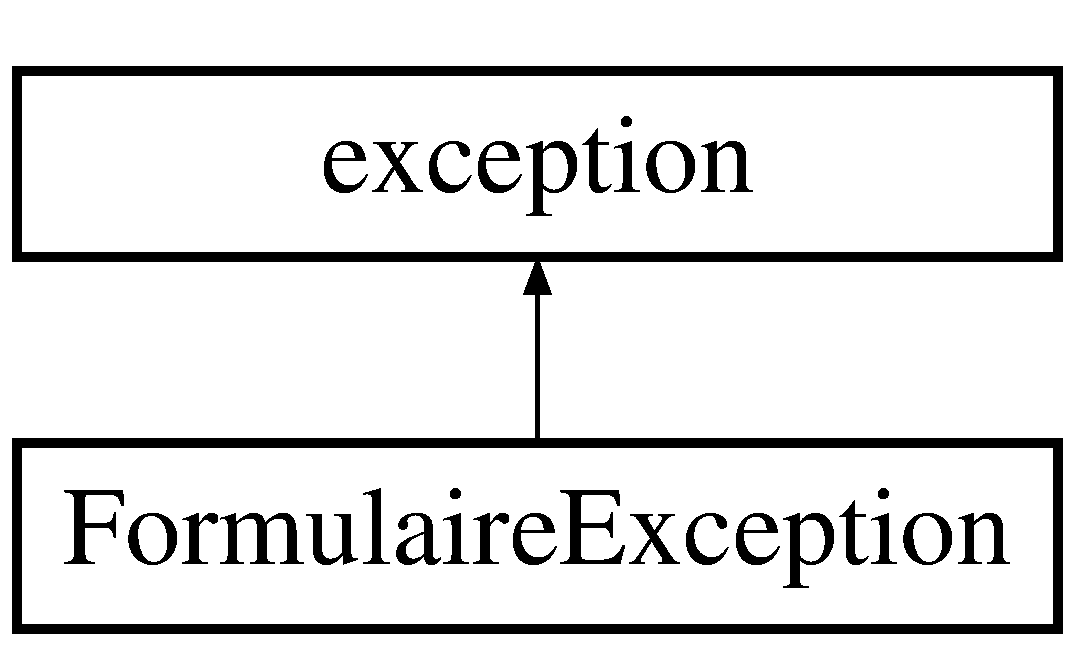
\includegraphics[height=2.000000cm]{class_formulaire_exception}
\end{center}
\end{figure}
\subsection*{Fonctions membres publiques}
\begin{DoxyCompactItemize}
\item 
\hypertarget{class_formulaire_exception_a4481db2c2d3fd6efe8a155133f19c75e}{{\bfseries Formulaire\+Exception} (const Q\+String \&i=\char`\"{}\char`\"{})  throw ()}\label{class_formulaire_exception_a4481db2c2d3fd6efe8a155133f19c75e}

\item 
\hypertarget{class_formulaire_exception_a067f6b72ade9697de1554549de535631}{Q\+String {\bfseries getinfo} () const   throw ()}\label{class_formulaire_exception_a067f6b72ade9697de1554549de535631}

\end{DoxyCompactItemize}
\subsection*{Attributs protégés}
\begin{DoxyCompactItemize}
\item 
\hypertarget{class_formulaire_exception_aebcd242ecf3368163947e8ba41c1f997}{Q\+String {\bfseries info}}\label{class_formulaire_exception_aebcd242ecf3368163947e8ba41c1f997}

\end{DoxyCompactItemize}


La documentation de cette classe a été générée à partir du fichier suivant \+:\begin{DoxyCompactItemize}
\item 
formulaire.\+h\end{DoxyCompactItemize}

\hypertarget{class_inscription}{\section{Référence de la classe Inscription}
\label{class_inscription}\index{Inscription@{Inscription}}
}
Graphe d'héritage de Inscription\+:\begin{figure}[H]
\begin{center}
\leavevmode
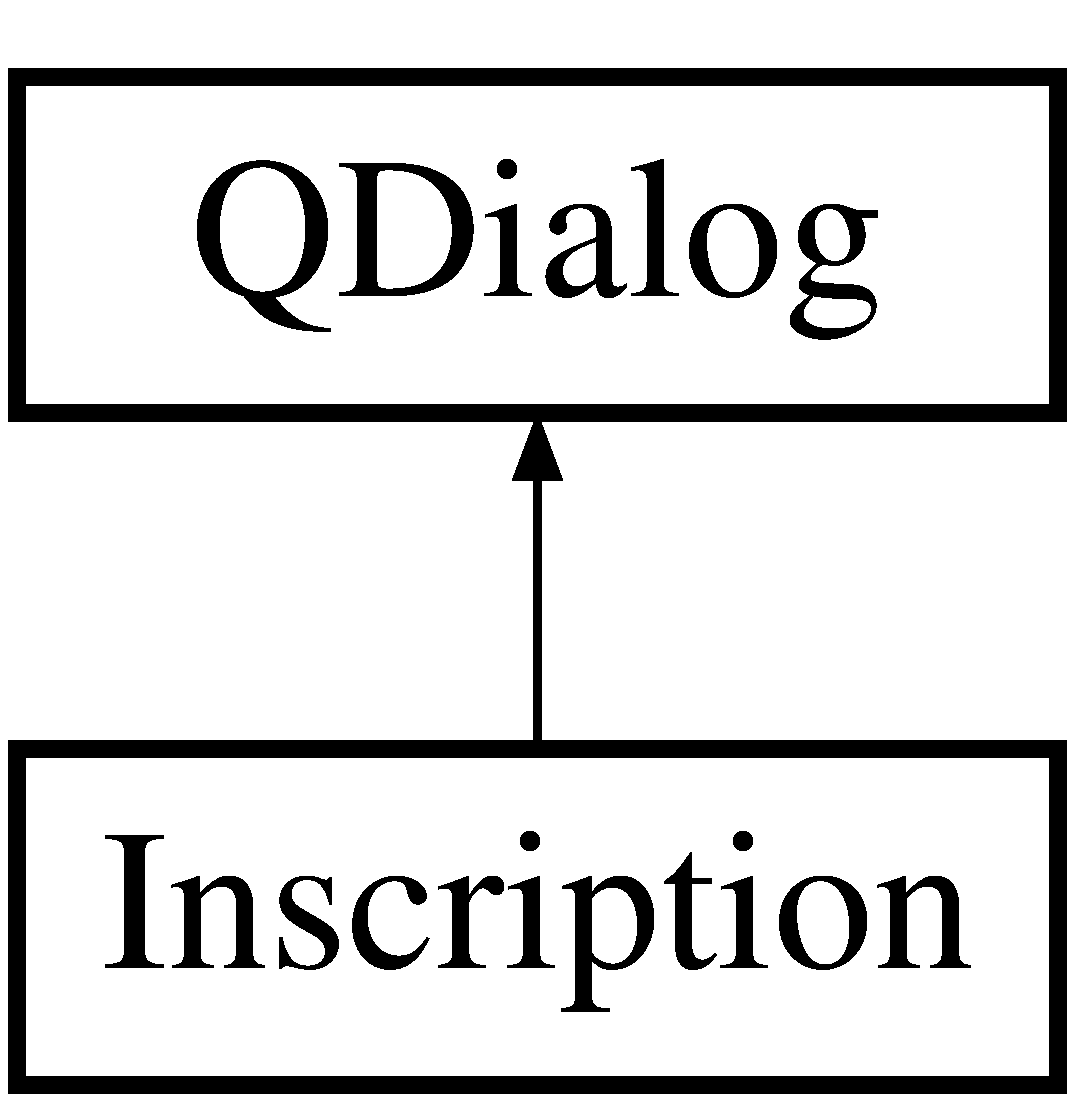
\includegraphics[height=2.000000cm]{class_inscription}
\end{center}
\end{figure}
\subsection*{Fonctions membres publiques}
\begin{DoxyCompactItemize}
\item 
\hypertarget{class_inscription_a608f9a8a73afa7fd640eb6c9e1dd0c64}{{\bfseries Inscription} (Q\+Widget $\ast$parent=0)}\label{class_inscription_a608f9a8a73afa7fd640eb6c9e1dd0c64}

\item 
\hypertarget{class_inscription_ae5813a1c17301c0c3638fc8c67558eb4}{{\bfseries Inscription} (const \hyperlink{class_u_v}{U\+V} \&u, const \hyperlink{class_semestre}{Semestre} \&s, \hyperlink{class_note}{Note} res=E\+C)}\label{class_inscription_ae5813a1c17301c0c3638fc8c67558eb4}

\item 
\hypertarget{class_inscription_a02c7a282ebfc86a0f11989965d5f6b46}{const \hyperlink{class_u_v}{U\+V} \& {\bfseries get\+U\+V} () const }\label{class_inscription_a02c7a282ebfc86a0f11989965d5f6b46}

\item 
\hypertarget{class_inscription_a04fc765bec80a60f65f07af72de90ea7}{\hyperlink{class_semestre}{Semestre} {\bfseries get\+Semestre} () const }\label{class_inscription_a04fc765bec80a60f65f07af72de90ea7}

\item 
\hypertarget{class_inscription_a71bda789e8159491e35b924a59b4175b}{\hyperlink{class_note}{Note} {\bfseries get\+Resultat} () const }\label{class_inscription_a71bda789e8159491e35b924a59b4175b}

\item 
\hypertarget{class_inscription_a7236d5c2ea9bfc08d01bdfdb8ed851ec}{void {\bfseries set\+Resultat} (\hyperlink{class_note}{Note} newres)}\label{class_inscription_a7236d5c2ea9bfc08d01bdfdb8ed851ec}

\end{DoxyCompactItemize}


La documentation de cette classe a été générée à partir des fichiers suivants \+:\begin{DoxyCompactItemize}
\item 
inscription.\+h\item 
uvmanager.\+h\item 
inscription.\+cpp\end{DoxyCompactItemize}

\hypertarget{class_ui_1_1_inscription}{\section{Référence de la classe Ui\+:\+:Inscription}
\label{class_ui_1_1_inscription}\index{Ui\+::\+Inscription@{Ui\+::\+Inscription}}
}
Graphe d'héritage de Ui\+:\+:Inscription\+:\begin{figure}[H]
\begin{center}
\leavevmode
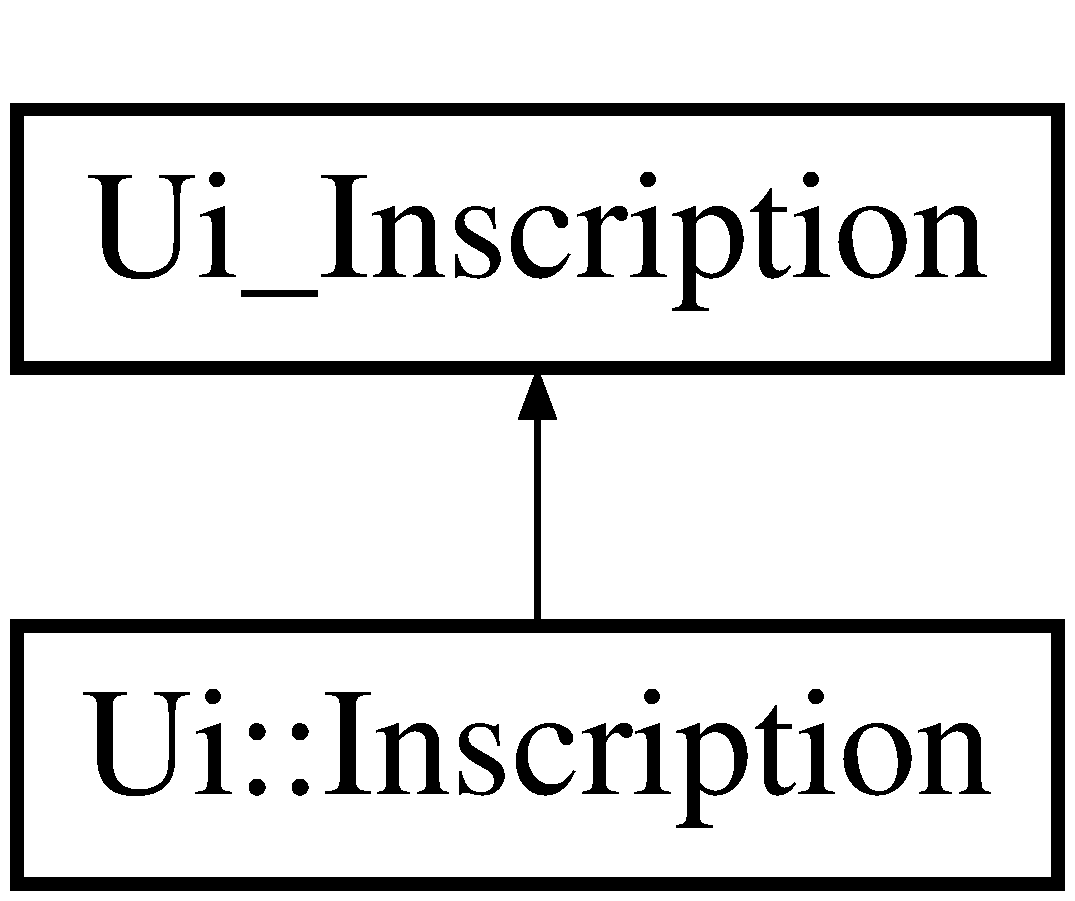
\includegraphics[height=2.000000cm]{class_ui_1_1_inscription}
\end{center}
\end{figure}
\subsection*{Membres hérités additionnels}


La documentation de cette classe a été générée à partir du fichier suivant \+:\begin{DoxyCompactItemize}
\item 
ui\+\_\+inscription.\+h\end{DoxyCompactItemize}

\hypertarget{class_insert_uv}{\section{Référence de la classe Insert\+Uv}
\label{class_insert_uv}\index{Insert\+Uv@{Insert\+Uv}}
}
Graphe d'héritage de Insert\+Uv\+:\begin{figure}[H]
\begin{center}
\leavevmode
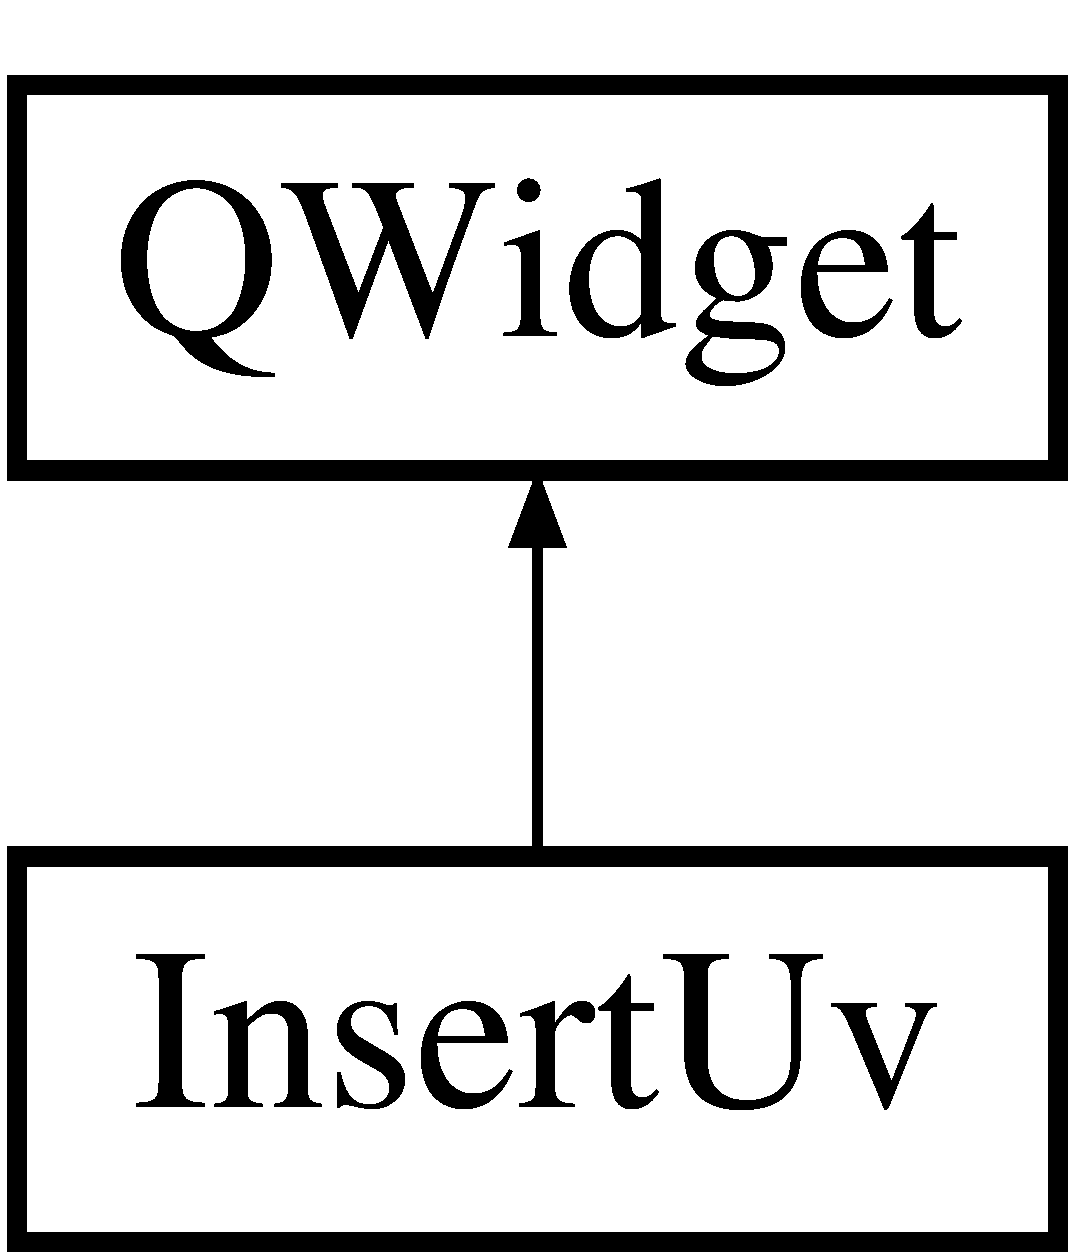
\includegraphics[height=2.000000cm]{class_insert_uv}
\end{center}
\end{figure}
\subsection*{Fonctions membres publiques}
\begin{DoxyCompactItemize}
\item 
\hypertarget{class_insert_uv_aa3b48991cf4a591a2f9c76411800b26b}{{\bfseries Insert\+Uv} (Q\+Widget $\ast$parent=0)}\label{class_insert_uv_aa3b48991cf4a591a2f9c76411800b26b}

\end{DoxyCompactItemize}


La documentation de cette classe a été générée à partir des fichiers suivants \+:\begin{DoxyCompactItemize}
\item 
insertuv.\+h\item 
insertuv.\+cpp\end{DoxyCompactItemize}

\hypertarget{class_ui_1_1_insert_uv}{\section{Référence de la classe Ui\+:\+:Insert\+Uv}
\label{class_ui_1_1_insert_uv}\index{Ui\+::\+Insert\+Uv@{Ui\+::\+Insert\+Uv}}
}
Graphe d'héritage de Ui\+:\+:Insert\+Uv\+:\begin{figure}[H]
\begin{center}
\leavevmode
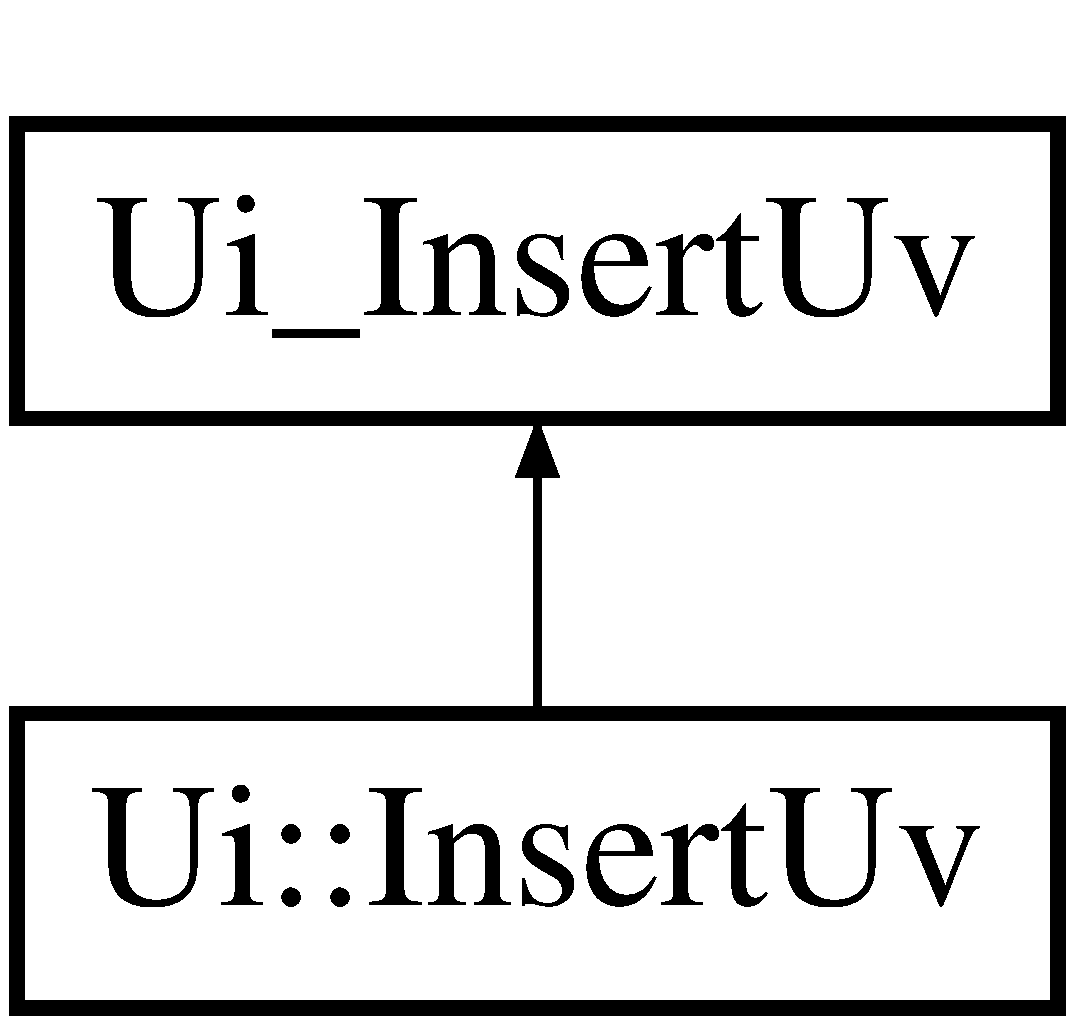
\includegraphics[height=2.000000cm]{class_ui_1_1_insert_uv}
\end{center}
\end{figure}
\subsection*{Membres hérités additionnels}


La documentation de cette classe a été générée à partir du fichier suivant \+:\begin{DoxyCompactItemize}
\item 
ui\+\_\+insertuv.\+h\end{DoxyCompactItemize}

\hypertarget{class_u_v_manager_1_1_iterator}{\section{Référence de la classe U\+V\+Manager\+:\+:Iterator}
\label{class_u_v_manager_1_1_iterator}\index{U\+V\+Manager\+::\+Iterator@{U\+V\+Manager\+::\+Iterator}}
}
\subsection*{Fonctions membres publiques}
\begin{DoxyCompactItemize}
\item 
\hypertarget{class_u_v_manager_1_1_iterator_a3ec3a33ce7a203f1cfe41e270c2d5618}{bool {\bfseries is\+Done} () const }\label{class_u_v_manager_1_1_iterator_a3ec3a33ce7a203f1cfe41e270c2d5618}

\item 
\hypertarget{class_u_v_manager_1_1_iterator_a01d51088890a5e83e96407bbc5ca919e}{void {\bfseries next} ()}\label{class_u_v_manager_1_1_iterator_a01d51088890a5e83e96407bbc5ca919e}

\item 
\hypertarget{class_u_v_manager_1_1_iterator_a1629af42307532caed05e2bec601d48d}{\hyperlink{class_u_v}{U\+V} \& {\bfseries current} () const }\label{class_u_v_manager_1_1_iterator_a1629af42307532caed05e2bec601d48d}

\end{DoxyCompactItemize}
\subsection*{Amis}
\begin{DoxyCompactItemize}
\item 
\hypertarget{class_u_v_manager_1_1_iterator_a335ec2026467669b89518b0c67372f3b}{class {\bfseries U\+V\+Manager}}\label{class_u_v_manager_1_1_iterator_a335ec2026467669b89518b0c67372f3b}

\end{DoxyCompactItemize}


La documentation de cette classe a été générée à partir du fichier suivant \+:\begin{DoxyCompactItemize}
\item 
uvmanager.\+h\end{DoxyCompactItemize}

\hypertarget{class_u_v_manager_1_1iterator}{\section{Référence de la classe U\+V\+Manager\+:\+:iterator}
\label{class_u_v_manager_1_1iterator}\index{U\+V\+Manager\+::iterator@{U\+V\+Manager\+::iterator}}
}
\subsection*{Fonctions membres publiques}
\begin{DoxyCompactItemize}
\item 
\hypertarget{class_u_v_manager_1_1iterator_aba2cf7041889369cada80deae4610c41}{\hyperlink{class_u_v}{U\+V} \& {\bfseries operator$\ast$} () const }\label{class_u_v_manager_1_1iterator_aba2cf7041889369cada80deae4610c41}

\item 
\hypertarget{class_u_v_manager_1_1iterator_ac3c9ff57c41e30982cf1d14fe98d1572}{bool {\bfseries operator!=} (\hyperlink{class_u_v_manager_1_1iterator}{iterator} it) const }\label{class_u_v_manager_1_1iterator_ac3c9ff57c41e30982cf1d14fe98d1572}

\item 
\hypertarget{class_u_v_manager_1_1iterator_a9f5057184b78bd6d3298251f282e5a90}{\hyperlink{class_u_v_manager_1_1iterator}{iterator} \& {\bfseries operator++} ()}\label{class_u_v_manager_1_1iterator_a9f5057184b78bd6d3298251f282e5a90}

\end{DoxyCompactItemize}
\subsection*{Amis}
\begin{DoxyCompactItemize}
\item 
\hypertarget{class_u_v_manager_1_1iterator_a335ec2026467669b89518b0c67372f3b}{class {\bfseries U\+V\+Manager}}\label{class_u_v_manager_1_1iterator_a335ec2026467669b89518b0c67372f3b}

\end{DoxyCompactItemize}


La documentation de cette classe a été générée à partir du fichier suivant \+:\begin{DoxyCompactItemize}
\item 
uvmanager.\+h\end{DoxyCompactItemize}

\hypertarget{class_ui_1_1mondossier}{\section{Référence de la classe Ui\+:\+:mondossier}
\label{class_ui_1_1mondossier}\index{Ui\+::mondossier@{Ui\+::mondossier}}
}
Graphe d'héritage de Ui\+:\+:mondossier\+:\begin{figure}[H]
\begin{center}
\leavevmode
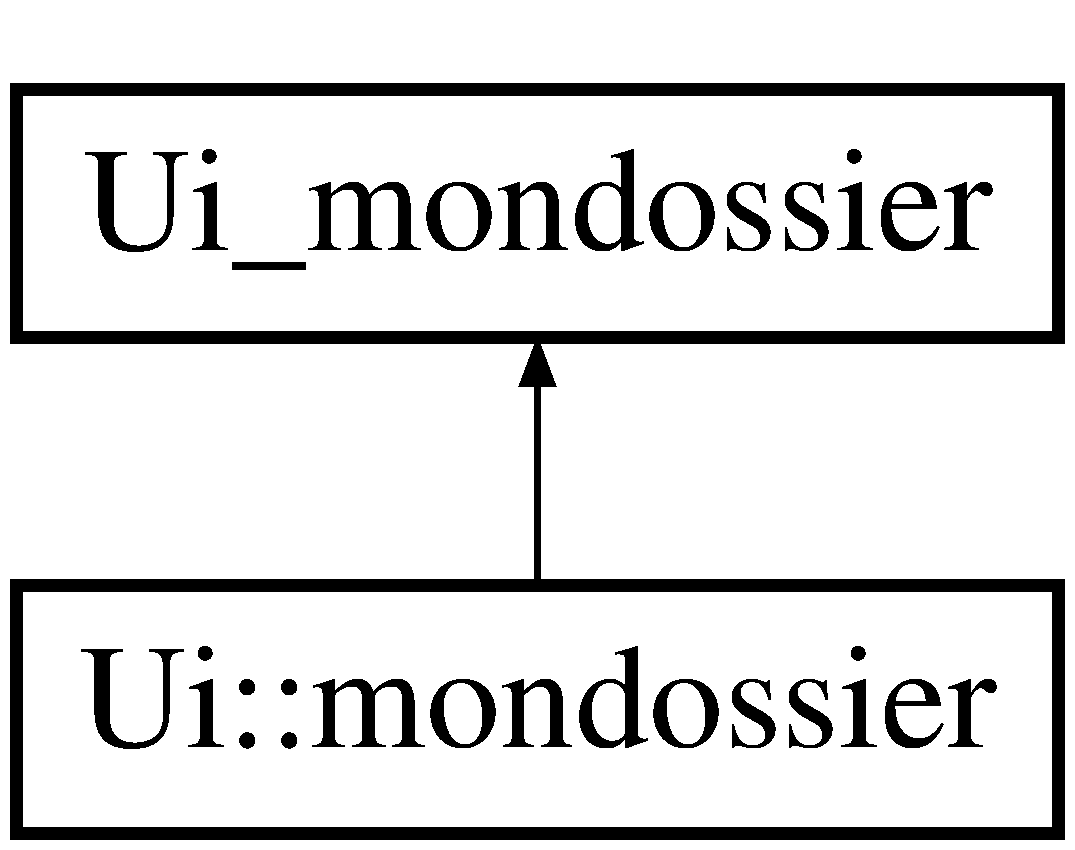
\includegraphics[height=2.000000cm]{class_ui_1_1mondossier}
\end{center}
\end{figure}
\subsection*{Membres hérités additionnels}


La documentation de cette classe a été générée à partir du fichier suivant \+:\begin{DoxyCompactItemize}
\item 
ui\+\_\+mondossier.\+h\end{DoxyCompactItemize}

\hypertarget{classmondossier}{\section{Référence de la classe mondossier}
\label{classmondossier}\index{mondossier@{mondossier}}
}
Graphe d'héritage de mondossier\+:\begin{figure}[H]
\begin{center}
\leavevmode
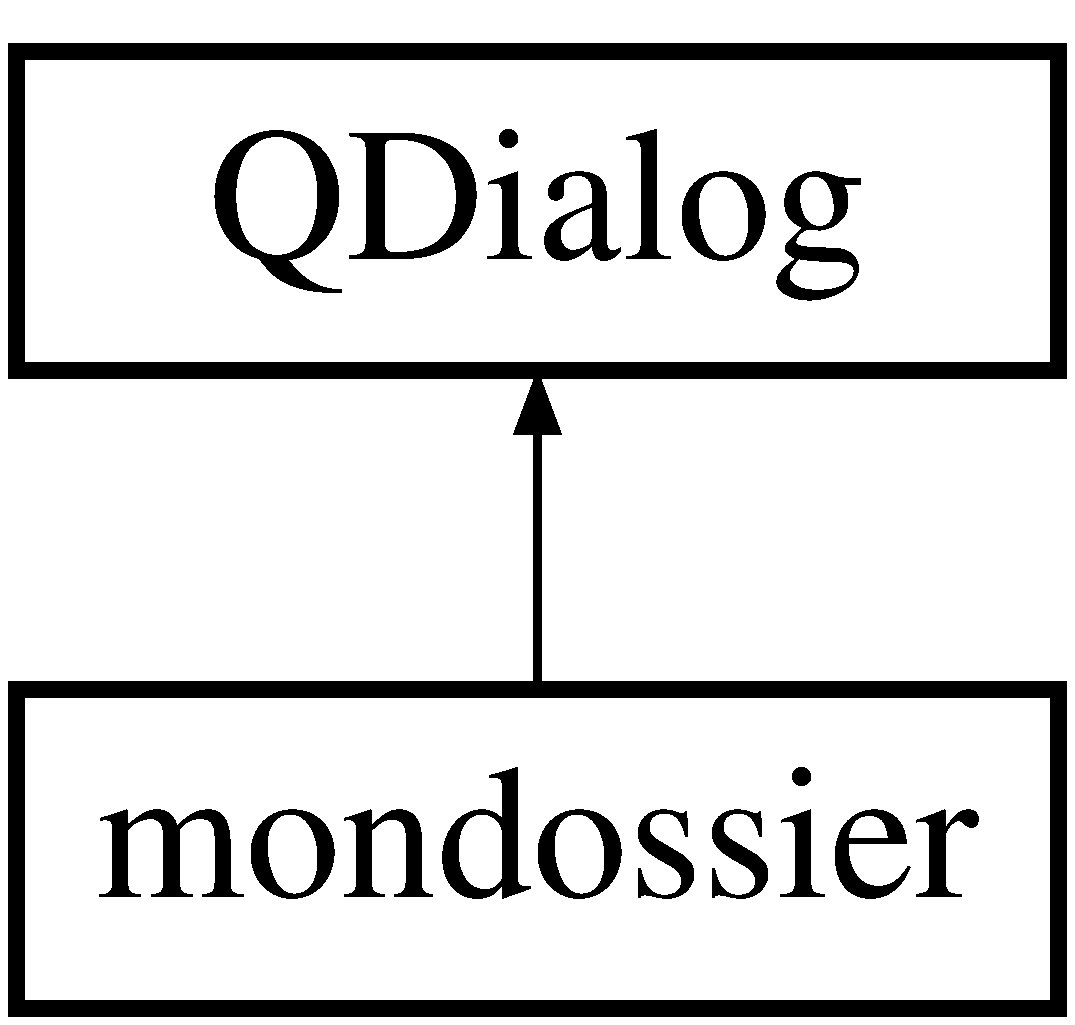
\includegraphics[height=2.000000cm]{classmondossier}
\end{center}
\end{figure}
\subsection*{Connecteurs publics}
\begin{DoxyCompactItemize}
\item 
\hypertarget{classmondossier_ab6c2f44ffadf1a30d025e0e2fef32f68}{void {\bfseries maj\+\_\+dossier} ()}\label{classmondossier_ab6c2f44ffadf1a30d025e0e2fef32f68}

\end{DoxyCompactItemize}
\subsection*{Fonctions membres publiques}
\begin{DoxyCompactItemize}
\item 
\hypertarget{classmondossier_a79af90264af161c9d8bb34e53b17f464}{{\bfseries mondossier} (Q\+Widget $\ast$parent=0)}\label{classmondossier_a79af90264af161c9d8bb34e53b17f464}

\item 
\hypertarget{classmondossier_ac434ae06e3bf4021952d5d649529190b}{void {\bfseries remplirchoix} ()}\label{classmondossier_ac434ae06e3bf4021952d5d649529190b}

\item 
\hypertarget{classmondossier_ad82e53838f6ff329bfa24ea1236ab32d}{void {\bfseries rempliruvsuivies} ()}\label{classmondossier_ad82e53838f6ff329bfa24ea1236ab32d}

\end{DoxyCompactItemize}


La documentation de cette classe a été générée à partir des fichiers suivants \+:\begin{DoxyCompactItemize}
\item 
mondossier.\+h\item 
mondossier.\+cpp\end{DoxyCompactItemize}

\hypertarget{class_note}{\section{Référence de la classe Note}
\label{class_note}\index{Note@{Note}}
}
\subsection*{Fonctions membres publiques}
\begin{DoxyCompactItemize}
\item 
\hypertarget{class_note_a59ccedfa5152470ea7ed600f0b34b423}{Q\+String\+List {\bfseries get\+Notes} () const }\label{class_note_a59ccedfa5152470ea7ed600f0b34b423}

\end{DoxyCompactItemize}


La documentation de cette classe a été générée à partir des fichiers suivants \+:\begin{DoxyCompactItemize}
\item 
note.\+h\item 
note.\+cpp\end{DoxyCompactItemize}

\hypertarget{structqt__meta__stringdata___accueil__t}{\section{Référence de la structure qt\+\_\+meta\+\_\+stringdata\+\_\+\+Accueil\+\_\+t}
\label{structqt__meta__stringdata___accueil__t}\index{qt\+\_\+meta\+\_\+stringdata\+\_\+\+Accueil\+\_\+t@{qt\+\_\+meta\+\_\+stringdata\+\_\+\+Accueil\+\_\+t}}
}
\subsection*{Attributs publics}
\begin{DoxyCompactItemize}
\item 
\hypertarget{structqt__meta__stringdata___accueil__t_aa3c8066f1a50a643db8e1e5dc301cb9f}{Q\+Byte\+Array\+Data {\bfseries data} \mbox{[}5\mbox{]}}\label{structqt__meta__stringdata___accueil__t_aa3c8066f1a50a643db8e1e5dc301cb9f}

\item 
\hypertarget{structqt__meta__stringdata___accueil__t_a9af13560b0f4dd3dd3a759e3feb2af1d}{char {\bfseries stringdata} \mbox{[}51\mbox{]}}\label{structqt__meta__stringdata___accueil__t_a9af13560b0f4dd3dd3a759e3feb2af1d}

\end{DoxyCompactItemize}


La documentation de cette structure a été générée à partir du fichier suivant \+:\begin{DoxyCompactItemize}
\item 
moc\+\_\+accueil.\+cpp\end{DoxyCompactItemize}

\hypertarget{structqt__meta__stringdata___administration__t}{\section{Référence de la structure qt\+\_\+meta\+\_\+stringdata\+\_\+\+Administration\+\_\+t}
\label{structqt__meta__stringdata___administration__t}\index{qt\+\_\+meta\+\_\+stringdata\+\_\+\+Administration\+\_\+t@{qt\+\_\+meta\+\_\+stringdata\+\_\+\+Administration\+\_\+t}}
}
\subsection*{Attributs publics}
\begin{DoxyCompactItemize}
\item 
\hypertarget{structqt__meta__stringdata___administration__t_a4043854211d9257b14b5b19133b1188f}{Q\+Byte\+Array\+Data {\bfseries data} \mbox{[}57\mbox{]}}\label{structqt__meta__stringdata___administration__t_a4043854211d9257b14b5b19133b1188f}

\item 
\hypertarget{structqt__meta__stringdata___administration__t_a4b76ebd7af4e2060e221ffed227989cc}{char {\bfseries stringdata} \mbox{[}1075\mbox{]}}\label{structqt__meta__stringdata___administration__t_a4b76ebd7af4e2060e221ffed227989cc}

\end{DoxyCompactItemize}


La documentation de cette structure a été générée à partir du fichier suivant \+:\begin{DoxyCompactItemize}
\item 
moc\+\_\+administration.\+cpp\end{DoxyCompactItemize}

\hypertarget{structqt__meta__stringdata__detailuv__t}{\section{Référence de la structure qt\+\_\+meta\+\_\+stringdata\+\_\+detailuv\+\_\+t}
\label{structqt__meta__stringdata__detailuv__t}\index{qt\+\_\+meta\+\_\+stringdata\+\_\+detailuv\+\_\+t@{qt\+\_\+meta\+\_\+stringdata\+\_\+detailuv\+\_\+t}}
}
\subsection*{Attributs publics}
\begin{DoxyCompactItemize}
\item 
\hypertarget{structqt__meta__stringdata__detailuv__t_a79bd25ae054fe9d5115c1bae9e037ea9}{Q\+Byte\+Array\+Data {\bfseries data} \mbox{[}1\mbox{]}}\label{structqt__meta__stringdata__detailuv__t_a79bd25ae054fe9d5115c1bae9e037ea9}

\item 
\hypertarget{structqt__meta__stringdata__detailuv__t_adad5b2e6666f20c530592ddc9b43800e}{char {\bfseries stringdata} \mbox{[}10\mbox{]}}\label{structqt__meta__stringdata__detailuv__t_adad5b2e6666f20c530592ddc9b43800e}

\end{DoxyCompactItemize}


La documentation de cette structure a été générée à partir du fichier suivant \+:\begin{DoxyCompactItemize}
\item 
moc\+\_\+detailuv.\+cpp\end{DoxyCompactItemize}

\hypertarget{structqt__meta__stringdata__fenetreplus__t}{\section{Référence de la structure qt\+\_\+meta\+\_\+stringdata\+\_\+fenetreplus\+\_\+t}
\label{structqt__meta__stringdata__fenetreplus__t}\index{qt\+\_\+meta\+\_\+stringdata\+\_\+fenetreplus\+\_\+t@{qt\+\_\+meta\+\_\+stringdata\+\_\+fenetreplus\+\_\+t}}
}
\subsection*{Attributs publics}
\begin{DoxyCompactItemize}
\item 
\hypertarget{structqt__meta__stringdata__fenetreplus__t_aedbfcc580cbb7ec354e17fe2ff1144e3}{Q\+Byte\+Array\+Data {\bfseries data} \mbox{[}4\mbox{]}}\label{structqt__meta__stringdata__fenetreplus__t_aedbfcc580cbb7ec354e17fe2ff1144e3}

\item 
\hypertarget{structqt__meta__stringdata__fenetreplus__t_a0c8a12da1137c90c77141f4efa671b87}{char {\bfseries stringdata} \mbox{[}44\mbox{]}}\label{structqt__meta__stringdata__fenetreplus__t_a0c8a12da1137c90c77141f4efa671b87}

\end{DoxyCompactItemize}


La documentation de cette structure a été générée à partir du fichier suivant \+:\begin{DoxyCompactItemize}
\item 
moc\+\_\+fenetreplus.\+cpp\end{DoxyCompactItemize}

\hypertarget{structqt__meta__stringdata___inscription__t}{\section{Référence de la structure qt\+\_\+meta\+\_\+stringdata\+\_\+\+Inscription\+\_\+t}
\label{structqt__meta__stringdata___inscription__t}\index{qt\+\_\+meta\+\_\+stringdata\+\_\+\+Inscription\+\_\+t@{qt\+\_\+meta\+\_\+stringdata\+\_\+\+Inscription\+\_\+t}}
}
\subsection*{Attributs publics}
\begin{DoxyCompactItemize}
\item 
\hypertarget{structqt__meta__stringdata___inscription__t_aca8da12b97d183c10a5383887c330c86}{Q\+Byte\+Array\+Data {\bfseries data} \mbox{[}3\mbox{]}}\label{structqt__meta__stringdata___inscription__t_aca8da12b97d183c10a5383887c330c86}

\item 
\hypertarget{structqt__meta__stringdata___inscription__t_ac3371c007e2d62147816a92a670aec35}{char {\bfseries stringdata} \mbox{[}30\mbox{]}}\label{structqt__meta__stringdata___inscription__t_ac3371c007e2d62147816a92a670aec35}

\end{DoxyCompactItemize}


La documentation de cette structure a été générée à partir du fichier suivant \+:\begin{DoxyCompactItemize}
\item 
moc\+\_\+inscription.\+cpp\end{DoxyCompactItemize}

\hypertarget{structqt__meta__stringdata___insert_uv__t}{\section{Référence de la structure qt\+\_\+meta\+\_\+stringdata\+\_\+\+Insert\+Uv\+\_\+t}
\label{structqt__meta__stringdata___insert_uv__t}\index{qt\+\_\+meta\+\_\+stringdata\+\_\+\+Insert\+Uv\+\_\+t@{qt\+\_\+meta\+\_\+stringdata\+\_\+\+Insert\+Uv\+\_\+t}}
}
\subsection*{Attributs publics}
\begin{DoxyCompactItemize}
\item 
\hypertarget{structqt__meta__stringdata___insert_uv__t_a56bcae759c1d2f4bc62388aa48578642}{Q\+Byte\+Array\+Data {\bfseries data} \mbox{[}1\mbox{]}}\label{structqt__meta__stringdata___insert_uv__t_a56bcae759c1d2f4bc62388aa48578642}

\item 
\hypertarget{structqt__meta__stringdata___insert_uv__t_aa5aea9c059c9f16fa76c554ca0722d10}{char {\bfseries stringdata} \mbox{[}10\mbox{]}}\label{structqt__meta__stringdata___insert_uv__t_aa5aea9c059c9f16fa76c554ca0722d10}

\end{DoxyCompactItemize}


La documentation de cette structure a été générée à partir du fichier suivant \+:\begin{DoxyCompactItemize}
\item 
moc\+\_\+insertuv.\+cpp\end{DoxyCompactItemize}

\hypertarget{structqt__meta__stringdata__mondossier__t}{\section{Référence de la structure qt\+\_\+meta\+\_\+stringdata\+\_\+mondossier\+\_\+t}
\label{structqt__meta__stringdata__mondossier__t}\index{qt\+\_\+meta\+\_\+stringdata\+\_\+mondossier\+\_\+t@{qt\+\_\+meta\+\_\+stringdata\+\_\+mondossier\+\_\+t}}
}
\subsection*{Attributs publics}
\begin{DoxyCompactItemize}
\item 
\hypertarget{structqt__meta__stringdata__mondossier__t_ae7b9b24585d7c4b5197d5e0c07fabbda}{Q\+Byte\+Array\+Data {\bfseries data} \mbox{[}18\mbox{]}}\label{structqt__meta__stringdata__mondossier__t_ae7b9b24585d7c4b5197d5e0c07fabbda}

\item 
\hypertarget{structqt__meta__stringdata__mondossier__t_abd12e01fccd077176382c081677ff94e}{char {\bfseries stringdata} \mbox{[}248\mbox{]}}\label{structqt__meta__stringdata__mondossier__t_abd12e01fccd077176382c081677ff94e}

\end{DoxyCompactItemize}


La documentation de cette structure a été générée à partir du fichier suivant \+:\begin{DoxyCompactItemize}
\item 
moc\+\_\+mondossier.\+cpp\end{DoxyCompactItemize}

\hypertarget{structqt__meta__stringdata___view_uv__t}{\section{Référence de la structure qt\+\_\+meta\+\_\+stringdata\+\_\+\+View\+Uv\+\_\+t}
\label{structqt__meta__stringdata___view_uv__t}\index{qt\+\_\+meta\+\_\+stringdata\+\_\+\+View\+Uv\+\_\+t@{qt\+\_\+meta\+\_\+stringdata\+\_\+\+View\+Uv\+\_\+t}}
}
\subsection*{Attributs publics}
\begin{DoxyCompactItemize}
\item 
\hypertarget{structqt__meta__stringdata___view_uv__t_ab42cbbdbbab3a432b6540b7d3d0570b3}{Q\+Byte\+Array\+Data {\bfseries data} \mbox{[}1\mbox{]}}\label{structqt__meta__stringdata___view_uv__t_ab42cbbdbbab3a432b6540b7d3d0570b3}

\item 
\hypertarget{structqt__meta__stringdata___view_uv__t_aa930279d2eb22385ce54b9b77d0cd46f}{char {\bfseries stringdata} \mbox{[}8\mbox{]}}\label{structqt__meta__stringdata___view_uv__t_aa930279d2eb22385ce54b9b77d0cd46f}

\end{DoxyCompactItemize}


La documentation de cette structure a été générée à partir du fichier suivant \+:\begin{DoxyCompactItemize}
\item 
moc\+\_\+viewuv.\+cpp\end{DoxyCompactItemize}

\hypertarget{class_semestre}{\section{Référence de la classe Semestre}
\label{class_semestre}\index{Semestre@{Semestre}}
}
Graphe d'héritage de Semestre\+:\begin{figure}[H]
\begin{center}
\leavevmode
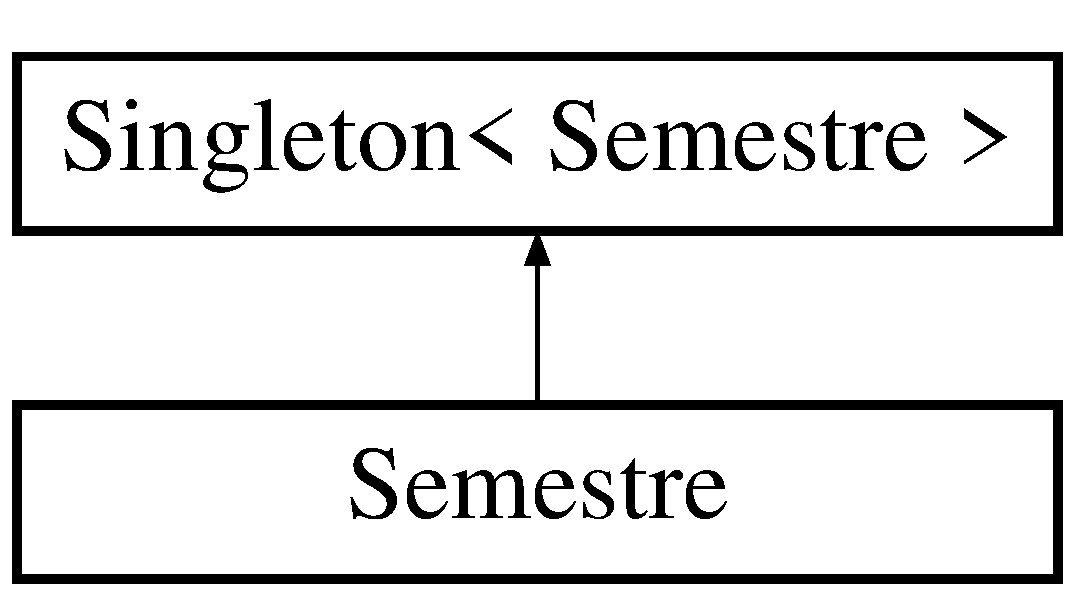
\includegraphics[height=2.000000cm]{class_semestre}
\end{center}
\end{figure}
\subsection*{Fonctions membres publiques}
\begin{DoxyCompactItemize}
\item 
\hypertarget{class_semestre_a9f78b2bd60c50f33226f741ff84a3d20}{Q\+String\+List \& {\bfseries get\+Liste\+\_\+semestres} ()}\label{class_semestre_a9f78b2bd60c50f33226f741ff84a3d20}

\item 
\hypertarget{class_semestre_afede7f0925e23cabac2625334450f50c}{void {\bfseries push\+\_\+back} (Q\+String item)}\label{class_semestre_afede7f0925e23cabac2625334450f50c}

\item 
\hypertarget{class_semestre_a82fa2036ff248389144a17dc73f6eb94}{void {\bfseries remove\+At} (int row)}\label{class_semestre_a82fa2036ff248389144a17dc73f6eb94}

\item 
\hypertarget{class_semestre_a276b752f301b59c8164528ef1e94a13e}{void {\bfseries set\+Liste\+\_\+semestres} (Q\+String\+List \&l)}\label{class_semestre_a276b752f301b59c8164528ef1e94a13e}

\item 
\hypertarget{class_semestre_a4a0f1d3ab2f65755e0e0f610526522c2}{{\bfseries Semestre} (Saison s, unsigned int a)}\label{class_semestre_a4a0f1d3ab2f65755e0e0f610526522c2}

\item 
\hypertarget{class_semestre_a26e25575e7fb65649c47970a9800c3aa}{Saison {\bfseries get\+Saison} () const }\label{class_semestre_a26e25575e7fb65649c47970a9800c3aa}

\item 
\hypertarget{class_semestre_a5aa85395e97f58f491ebf251da8231ef}{unsigned int {\bfseries get\+Annee} () const }\label{class_semestre_a5aa85395e97f58f491ebf251da8231ef}

\end{DoxyCompactItemize}
\subsection*{Amis}
\begin{DoxyCompactItemize}
\item 
\hypertarget{class_semestre_a7b353f5e61182b1b184df63b085726fb}{class {\bfseries Singleton$<$ Semestre $>$}}\label{class_semestre_a7b353f5e61182b1b184df63b085726fb}

\end{DoxyCompactItemize}
\subsection*{Membres hérités additionnels}


La documentation de cette classe a été générée à partir des fichiers suivants \+:\begin{DoxyCompactItemize}
\item 
semestre.\+h\item 
uvmanager.\+h\item 
semestre.\+cpp\end{DoxyCompactItemize}

\hypertarget{class_singleton}{\section{Référence du modèle de la classe Singleton$<$ T $>$}
\label{class_singleton}\index{Singleton$<$ T $>$@{Singleton$<$ T $>$}}
}
\subsection*{Fonctions membres publiques statiques}
\begin{DoxyCompactItemize}
\item 
\hypertarget{class_singleton_ad6f103597095efda360db4a230308666}{static T $\ast$ {\bfseries get\+Instance} ()}\label{class_singleton_ad6f103597095efda360db4a230308666}

\item 
\hypertarget{class_singleton_ac2686bdea2194fe911e68c5765924d7a}{static void {\bfseries kill} ()}\label{class_singleton_ac2686bdea2194fe911e68c5765924d7a}

\end{DoxyCompactItemize}
\subsection*{Attributs protégés statiques}
\begin{DoxyCompactItemize}
\item 
\hypertarget{class_singleton_a13a24bdde309c713f98d86413f4c3f43}{static T $\ast$ {\bfseries \+\_\+singleton} = N\+U\+L\+L}\label{class_singleton_a13a24bdde309c713f98d86413f4c3f43}

\end{DoxyCompactItemize}


La documentation de cette classe a été générée à partir du fichier suivant \+:\begin{DoxyCompactItemize}
\item 
singleton.\+h\end{DoxyCompactItemize}

\hypertarget{class_tools}{\section{Référence de la classe Tools}
\label{class_tools}\index{Tools@{Tools}}
}
\subsection*{Fonctions membres publiques statiques}
\begin{DoxyCompactItemize}
\item 
\hypertarget{class_tools_adfb1055387f11927667ad51da4b27d15}{static void {\bfseries switch\+\_\+current\+\_\+item} (Q\+List\+Widget $\ast$liste1, Q\+List\+Widget $\ast$liste2)}\label{class_tools_adfb1055387f11927667ad51da4b27d15}

\item 
\hypertarget{class_tools_adf2cfb0fe617825329e1a2c0082907e1}{static void {\bfseries enable\+\_\+combobox} (Q\+Combo\+Box $\ast$cbox, const Q\+String\+List \&liste)}\label{class_tools_adf2cfb0fe617825329e1a2c0082907e1}

\item 
\hypertarget{class_tools_a29902dd7872d4caf4ddd66435a3d335e}{static void {\bfseries maj\+\_\+liste} (Q\+List\+Widget $\ast$liste, Q\+Sql\+Query query)}\label{class_tools_a29902dd7872d4caf4ddd66435a3d335e}

\item 
\hypertarget{class_tools_aabd50fe50551005f43421a936643f748}{static void {\bfseries maj\+\_\+liste} (Q\+List\+Widget $\ast$liste1, Q\+List\+Widget $\ast$liste2, const Q\+Sql\+Query query)}\label{class_tools_aabd50fe50551005f43421a936643f748}

\end{DoxyCompactItemize}


La documentation de cette classe a été générée à partir des fichiers suivants \+:\begin{DoxyCompactItemize}
\item 
tools.\+h\item 
tools.\+cpp\end{DoxyCompactItemize}

\hypertarget{class_ui___accueil}{\section{Référence de la classe Ui\+\_\+\+Accueil}
\label{class_ui___accueil}\index{Ui\+\_\+\+Accueil@{Ui\+\_\+\+Accueil}}
}
Graphe d'héritage de Ui\+\_\+\+Accueil\+:\begin{figure}[H]
\begin{center}
\leavevmode
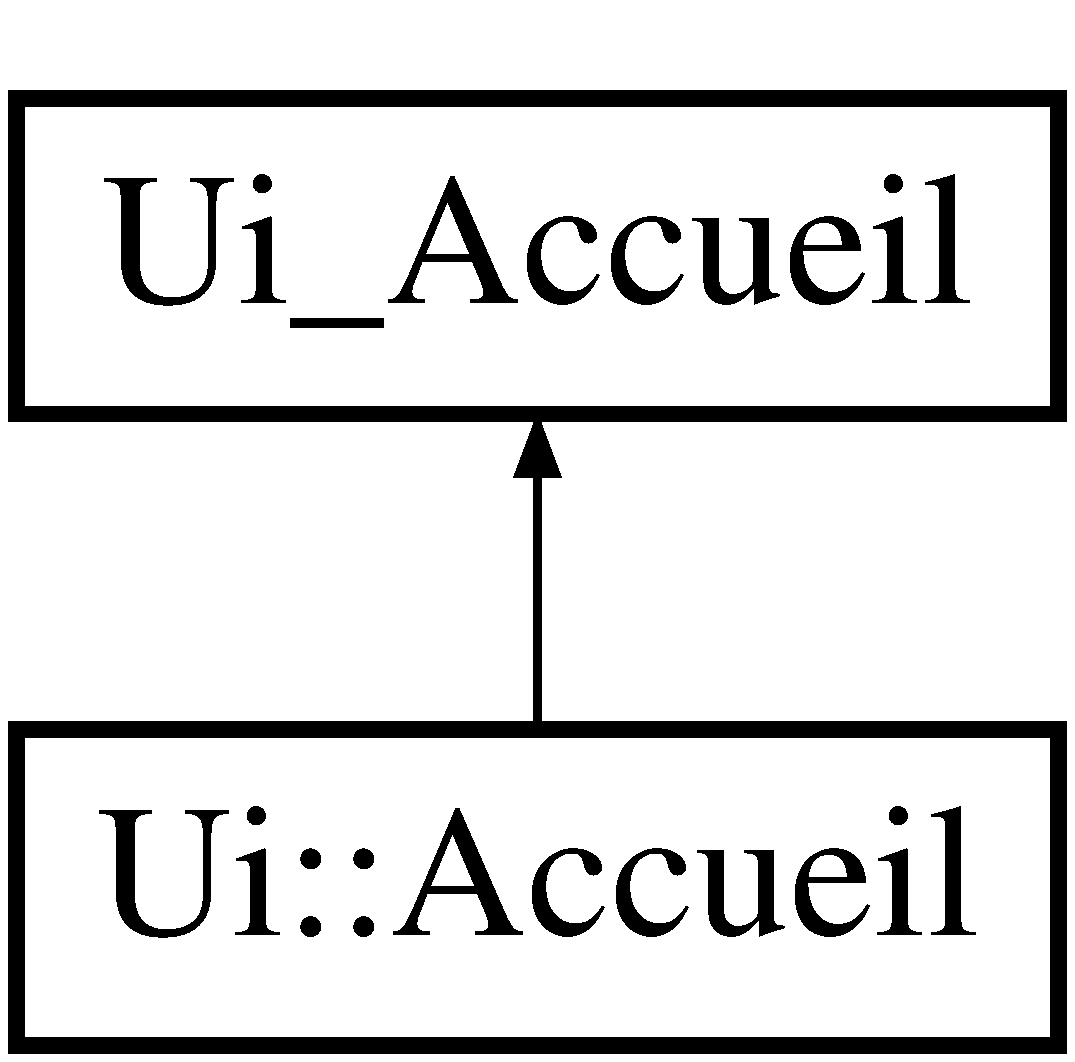
\includegraphics[height=2.000000cm]{class_ui___accueil}
\end{center}
\end{figure}
\subsection*{Fonctions membres publiques}
\begin{DoxyCompactItemize}
\item 
\hypertarget{class_ui___accueil_a7e4ac5dda22c0ee70dd5bb604335c9b2}{void {\bfseries setup\+Ui} (Q\+Main\+Window $\ast$\hyperlink{class_accueil}{Accueil})}\label{class_ui___accueil_a7e4ac5dda22c0ee70dd5bb604335c9b2}

\item 
\hypertarget{class_ui___accueil_af1be4e1d29cd4656ea9c5cf28eca03a8}{void {\bfseries retranslate\+Ui} (Q\+Main\+Window $\ast$\hyperlink{class_accueil}{Accueil})}\label{class_ui___accueil_af1be4e1d29cd4656ea9c5cf28eca03a8}

\end{DoxyCompactItemize}
\subsection*{Attributs publics}
\begin{DoxyCompactItemize}
\item 
\hypertarget{class_ui___accueil_a02d3942498c9d84b7080183e953905bc}{Q\+Widget $\ast$ {\bfseries centralwidget}}\label{class_ui___accueil_a02d3942498c9d84b7080183e953905bc}

\item 
\hypertarget{class_ui___accueil_a18adc2f4092065237f5c73195ce5d98c}{Q\+Tab\+Widget $\ast$ {\bfseries tab\+Widget}}\label{class_ui___accueil_a18adc2f4092065237f5c73195ce5d98c}

\item 
\hypertarget{class_ui___accueil_a0d5c8ac1fdae7ec3dd3b3f6b647a51da}{Q\+Widget $\ast$ {\bfseries Connexion}}\label{class_ui___accueil_a0d5c8ac1fdae7ec3dd3b3f6b647a51da}

\item 
\hypertarget{class_ui___accueil_aa7b30e2ee6bad3ab38fc8618ee943207}{Q\+Label $\ast$ {\bfseries label\+\_\+2}}\label{class_ui___accueil_aa7b30e2ee6bad3ab38fc8618ee943207}

\item 
\hypertarget{class_ui___accueil_a03264b45a8336ab30347be9d6b9571da}{Q\+Push\+Button $\ast$ {\bfseries inscription}}\label{class_ui___accueil_a03264b45a8336ab30347be9d6b9571da}

\item 
\hypertarget{class_ui___accueil_a61575c9676fc937a0396baf0e12753c7}{Q\+Line\+Edit $\ast$ {\bfseries input\+\_\+mdp}}\label{class_ui___accueil_a61575c9676fc937a0396baf0e12753c7}

\item 
\hypertarget{class_ui___accueil_aa46095a53a687dae54e90c92195871c3}{Q\+Line\+Edit $\ast$ {\bfseries input\+\_\+login}}\label{class_ui___accueil_aa46095a53a687dae54e90c92195871c3}

\item 
\hypertarget{class_ui___accueil_abcedabc678d6932f4402719bcb526214}{Q\+Label $\ast$ {\bfseries label\+\_\+mdp}}\label{class_ui___accueil_abcedabc678d6932f4402719bcb526214}

\item 
\hypertarget{class_ui___accueil_a3c87093c62386a45ac1718d6906f4a70}{Q\+Label $\ast$ {\bfseries label\+\_\+login}}\label{class_ui___accueil_a3c87093c62386a45ac1718d6906f4a70}

\item 
\hypertarget{class_ui___accueil_ad2788d40c70fc8dfa383dffc0a4154f6}{Q\+Push\+Button $\ast$ {\bfseries connexion}}\label{class_ui___accueil_ad2788d40c70fc8dfa383dffc0a4154f6}

\item 
\hypertarget{class_ui___accueil_a091534b4cb2843c4fa3612d1904a4ccf}{Q\+Label $\ast$ {\bfseries label\+\_\+erreur}}\label{class_ui___accueil_a091534b4cb2843c4fa3612d1904a4ccf}

\item 
\hypertarget{class_ui___accueil_ac3e85d9e0f053129791a9364b5db0490}{Q\+Label $\ast$ {\bfseries label}}\label{class_ui___accueil_ac3e85d9e0f053129791a9364b5db0490}

\item 
\hypertarget{class_ui___accueil_ae6f38fc28687f9f3b367a574c9c9328e}{Q\+Menu\+Bar $\ast$ {\bfseries menubar}}\label{class_ui___accueil_ae6f38fc28687f9f3b367a574c9c9328e}

\item 
\hypertarget{class_ui___accueil_a158e3fd627f6d680fc2d890d540a2a4f}{Q\+Status\+Bar $\ast$ {\bfseries statusbar}}\label{class_ui___accueil_a158e3fd627f6d680fc2d890d540a2a4f}

\end{DoxyCompactItemize}


La documentation de cette classe a été générée à partir du fichier suivant \+:\begin{DoxyCompactItemize}
\item 
ui\+\_\+accueil.\+h\end{DoxyCompactItemize}

\hypertarget{class_ui___administration}{\section{Référence de la classe Ui\+\_\+\+Administration}
\label{class_ui___administration}\index{Ui\+\_\+\+Administration@{Ui\+\_\+\+Administration}}
}
Graphe d'héritage de Ui\+\_\+\+Administration\+:\begin{figure}[H]
\begin{center}
\leavevmode
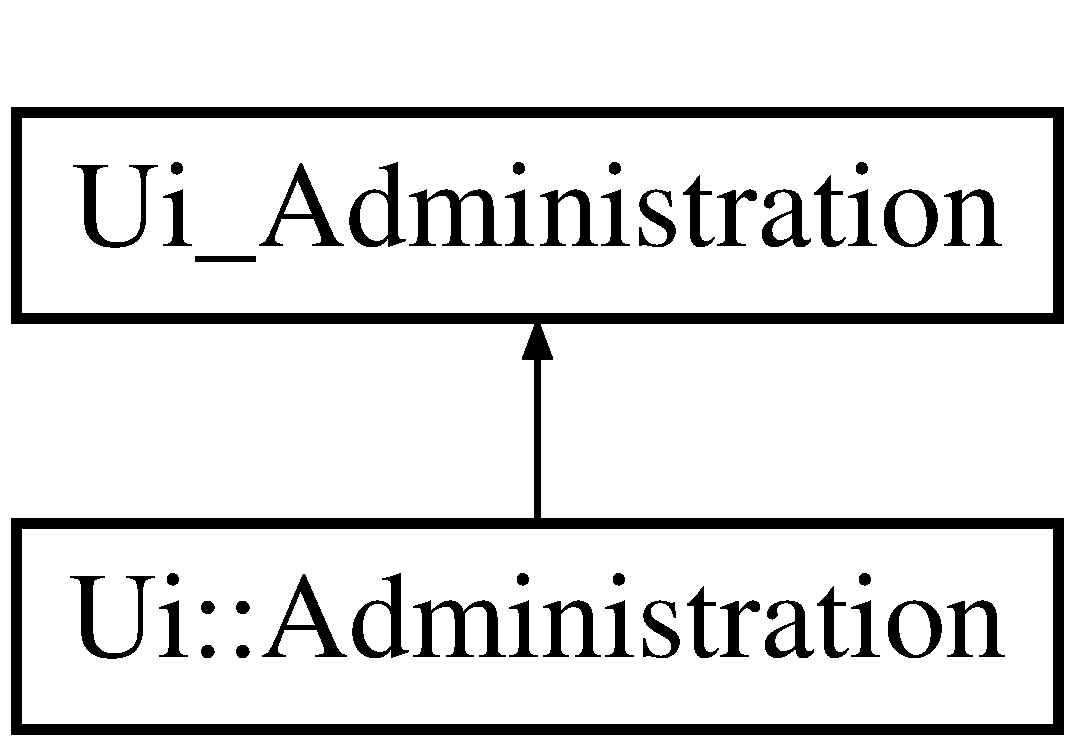
\includegraphics[height=2.000000cm]{class_ui___administration}
\end{center}
\end{figure}
\subsection*{Fonctions membres publiques}
\begin{DoxyCompactItemize}
\item 
\hypertarget{class_ui___administration_aed0321283112227dbfa74f4ba4870dc8}{void {\bfseries setup\+Ui} (Q\+Frame $\ast$\hyperlink{class_administration}{Administration})}\label{class_ui___administration_aed0321283112227dbfa74f4ba4870dc8}

\item 
\hypertarget{class_ui___administration_aef9aaf56620fbb3d0111a998c62e8558}{void {\bfseries retranslate\+Ui} (Q\+Frame $\ast$\hyperlink{class_administration}{Administration})}\label{class_ui___administration_aef9aaf56620fbb3d0111a998c62e8558}

\end{DoxyCompactItemize}
\subsection*{Attributs publics}
\begin{DoxyCompactItemize}
\item 
\hypertarget{class_ui___administration_a500ba19bf4813a712abe8fe3eac2f439}{Q\+Tab\+Widget $\ast$ {\bfseries onglets\+\_\+admin}}\label{class_ui___administration_a500ba19bf4813a712abe8fe3eac2f439}

\item 
\hypertarget{class_ui___administration_acd89460fb397f4d0d064fba4f80e93bf}{Q\+Widget $\ast$ {\bfseries gerer\+\_\+uv}}\label{class_ui___administration_acd89460fb397f4d0d064fba4f80e93bf}

\item 
\hypertarget{class_ui___administration_ab2ce200bb238057dbf42409933069ab2}{Q\+Tool\+Box $\ast$ {\bfseries tool\+Box\+\_\+uv}}\label{class_ui___administration_ab2ce200bb238057dbf42409933069ab2}

\item 
\hypertarget{class_ui___administration_a525a96ec8f92fe559948f9046ac78dbd}{Q\+Widget $\ast$ {\bfseries ajout\+\_\+uv}}\label{class_ui___administration_a525a96ec8f92fe559948f9046ac78dbd}

\item 
\hypertarget{class_ui___administration_a98cfaf57e23e941210f0b8e0e25c3348}{Q\+Label $\ast$ {\bfseries label\+\_\+ajout\+\_\+code\+\_\+uv}}\label{class_ui___administration_a98cfaf57e23e941210f0b8e0e25c3348}

\item 
\hypertarget{class_ui___administration_ae5e2591b45e6ebc27469107569e64121}{Q\+Text\+Edit $\ast$ {\bfseries ajout\+\_\+description\+\_\+uv}}\label{class_ui___administration_ae5e2591b45e6ebc27469107569e64121}

\item 
\hypertarget{class_ui___administration_ac71d7242c74540b4f1cf8a5a4a1ded7a}{Q\+Label $\ast$ {\bfseries label\+\_\+ajout\+\_\+description\+\_\+uv}}\label{class_ui___administration_ac71d7242c74540b4f1cf8a5a4a1ded7a}

\item 
\hypertarget{class_ui___administration_ad2bdfcc6cc68f15d764138938cdf5424}{Q\+Line\+Edit $\ast$ {\bfseries ajout\+\_\+code\+\_\+uv}}\label{class_ui___administration_ad2bdfcc6cc68f15d764138938cdf5424}

\item 
\hypertarget{class_ui___administration_a476c0465d7a4f6526a280ae43913745e}{Q\+Label $\ast$ {\bfseries titre\+\_\+ajout\+\_\+uv}}\label{class_ui___administration_a476c0465d7a4f6526a280ae43913745e}

\item 
\hypertarget{class_ui___administration_a8dd052324c85577cea76b3879f2b5f8f}{Q\+Push\+Button $\ast$ {\bfseries sauvegarder\+\_\+ajout\+\_\+uv}}\label{class_ui___administration_a8dd052324c85577cea76b3879f2b5f8f}

\item 
\hypertarget{class_ui___administration_a6999fa24ef66b74cc23008ac8919e767}{Q\+Group\+Box $\ast$ {\bfseries group\+\_\+ajout\+\_\+categorie\+\_\+uv}}\label{class_ui___administration_a6999fa24ef66b74cc23008ac8919e767}

\item 
\hypertarget{class_ui___administration_ae00200d0aa5983198c0d37c340b261f0}{Q\+Label $\ast$ {\bfseries label\+\_\+ajout\+\_\+categorie\+\_\+dispo\+\_\+uv}}\label{class_ui___administration_ae00200d0aa5983198c0d37c340b261f0}

\item 
\hypertarget{class_ui___administration_a465d8515bba8b4cf3a7cd0be9940c902}{Q\+List\+Widget $\ast$ {\bfseries liste\+\_\+ajout\+\_\+credits\+\_\+uv}}\label{class_ui___administration_a465d8515bba8b4cf3a7cd0be9940c902}

\item 
\hypertarget{class_ui___administration_a4c4fb9a7f637eeb52586bf25015ca5ac}{Q\+Label $\ast$ {\bfseries label\+\_\+ajout\+\_\+nb\+\_\+credits\+\_\+uv}}\label{class_ui___administration_a4c4fb9a7f637eeb52586bf25015ca5ac}

\item 
\hypertarget{class_ui___administration_a10c38560d243e3a814c6238ed68995ae}{Q\+Label $\ast$ {\bfseries label\+\_\+liste\+\_\+ajout\+\_\+credit\+\_\+uv}}\label{class_ui___administration_a10c38560d243e3a814c6238ed68995ae}

\item 
\hypertarget{class_ui___administration_a1bd575272efae72f58f3e8fa47bd67ee}{Q\+Push\+Button $\ast$ {\bfseries ajout\+\_\+categorie\+\_\+uv}}\label{class_ui___administration_a1bd575272efae72f58f3e8fa47bd67ee}

\item 
\hypertarget{class_ui___administration_aea8b5a9ebef832c562fe412a71f2b2f1}{Q\+Label $\ast$ {\bfseries label\+\_\+ajout\+\_\+categorie\+\_\+choisie\+\_\+uv}}\label{class_ui___administration_aea8b5a9ebef832c562fe412a71f2b2f1}

\item 
\hypertarget{class_ui___administration_ad6fd952aca8c348f02703d23c5b44544}{Q\+List\+Widget $\ast$ {\bfseries liste\+\_\+ajout\+\_\+categorie\+\_\+choisie\+\_\+uv}}\label{class_ui___administration_ad6fd952aca8c348f02703d23c5b44544}

\item 
\hypertarget{class_ui___administration_a706b48f017056ca88b4dec42aa34afdc}{Q\+Spin\+Box $\ast$ {\bfseries ajout\+\_\+credit\+\_\+uv}}\label{class_ui___administration_a706b48f017056ca88b4dec42aa34afdc}

\item 
\hypertarget{class_ui___administration_ae40405945047e71ccfa0790d7a177074}{Q\+Push\+Button $\ast$ {\bfseries retire\+\_\+categorie\+\_\+uv}}\label{class_ui___administration_ae40405945047e71ccfa0790d7a177074}

\item 
\hypertarget{class_ui___administration_a0f65b45d2b94a43e6af2649f2cd8ff5f}{Q\+List\+Widget $\ast$ {\bfseries liste\+\_\+ajout\+\_\+categorie\+\_\+dispo\+\_\+uv}}\label{class_ui___administration_a0f65b45d2b94a43e6af2649f2cd8ff5f}

\item 
\hypertarget{class_ui___administration_a9dd961b0085d5b052dc68994aee707d9}{Q\+Group\+Box $\ast$ {\bfseries group\+\_\+ajout\+\_\+filiere\+\_\+uv}}\label{class_ui___administration_a9dd961b0085d5b052dc68994aee707d9}

\item 
\hypertarget{class_ui___administration_a5bdb609c3cdbdc931b8ff950ec34fa36}{Q\+Label $\ast$ {\bfseries label\+\_\+ajout\+\_\+filiere\+\_\+dispo\+\_\+uv}}\label{class_ui___administration_a5bdb609c3cdbdc931b8ff950ec34fa36}

\item 
\hypertarget{class_ui___administration_a059665f26805da91ea5faec5810f3247}{Q\+Push\+Button $\ast$ {\bfseries ajout\+\_\+filiere\+\_\+uv}}\label{class_ui___administration_a059665f26805da91ea5faec5810f3247}

\item 
\hypertarget{class_ui___administration_a7f83feb7a28c3812d3cd0eadbb7cd709}{Q\+List\+Widget $\ast$ {\bfseries liste\+\_\+ajout\+\_\+filiere\+\_\+dispo\+\_\+uv}}\label{class_ui___administration_a7f83feb7a28c3812d3cd0eadbb7cd709}

\item 
\hypertarget{class_ui___administration_abeb653783b448abc941ec3c4b681e682}{Q\+List\+Widget $\ast$ {\bfseries liste\+\_\+ajout\+\_\+filiere\+\_\+choisie\+\_\+uv}}\label{class_ui___administration_abeb653783b448abc941ec3c4b681e682}

\item 
\hypertarget{class_ui___administration_a58089f73544db0a44fcce3e849ccd842}{Q\+Label $\ast$ {\bfseries label\+\_\+ajout\+\_\+filiere\+\_\+choisie\+\_\+uv}}\label{class_ui___administration_a58089f73544db0a44fcce3e849ccd842}

\item 
\hypertarget{class_ui___administration_a8f82296781ac968e60be4a98dab16334}{Q\+Push\+Button $\ast$ {\bfseries retire\+\_\+filiere\+\_\+uv}}\label{class_ui___administration_a8f82296781ac968e60be4a98dab16334}

\item 
\hypertarget{class_ui___administration_a7498fe123cad3268ad369eb50bed1a51}{Q\+Group\+Box $\ast$ {\bfseries group\+\_\+ajout\+\_\+branche\+\_\+uv}}\label{class_ui___administration_a7498fe123cad3268ad369eb50bed1a51}

\item 
\hypertarget{class_ui___administration_a11a235085e4d44ee7a84f8a869f51607}{Q\+Label $\ast$ {\bfseries label\+\_\+ajout\+\_\+branche\+\_\+choisie\+\_\+uv}}\label{class_ui___administration_a11a235085e4d44ee7a84f8a869f51607}

\item 
\hypertarget{class_ui___administration_a318d1a6a6f1608dfcb18722194585c11}{Q\+Push\+Button $\ast$ {\bfseries retire\+\_\+branche\+\_\+uv}}\label{class_ui___administration_a318d1a6a6f1608dfcb18722194585c11}

\item 
\hypertarget{class_ui___administration_a934906684788d00e4c3e61b16e45ff50}{Q\+Label $\ast$ {\bfseries label\+\_\+ajout\+\_\+branche\+\_\+uv}}\label{class_ui___administration_a934906684788d00e4c3e61b16e45ff50}

\item 
\hypertarget{class_ui___administration_ac395971c96a0da33bfcd243227aff24a}{Q\+List\+Widget $\ast$ {\bfseries liste\+\_\+ajout\+\_\+branche\+\_\+choisie\+\_\+uv}}\label{class_ui___administration_ac395971c96a0da33bfcd243227aff24a}

\item 
\hypertarget{class_ui___administration_af3c0697ab9173302211796cf3962ef4f}{Q\+List\+Widget $\ast$ {\bfseries liste\+\_\+ajout\+\_\+branche\+\_\+dispo\+\_\+uv}}\label{class_ui___administration_af3c0697ab9173302211796cf3962ef4f}

\item 
\hypertarget{class_ui___administration_ae2b13c15e1e6e4e43b1d033105b7b720}{Q\+Push\+Button $\ast$ {\bfseries ajout\+\_\+branche\+\_\+uv}}\label{class_ui___administration_ae2b13c15e1e6e4e43b1d033105b7b720}

\item 
\hypertarget{class_ui___administration_a6fd0bcc04355555d97c3d44a0dc6a7c3}{Q\+List\+Widget $\ast$ {\bfseries liste\+\_\+ajout\+\_\+obligation\+\_\+uv}}\label{class_ui___administration_a6fd0bcc04355555d97c3d44a0dc6a7c3}

\item 
\hypertarget{class_ui___administration_a88b825f66cf6616a4dc5f3901e72f43e}{Q\+Label $\ast$ {\bfseries label\+\_\+liste\+\_\+ajout\+\_\+obligation\+\_\+uv}}\label{class_ui___administration_a88b825f66cf6616a4dc5f3901e72f43e}

\item 
\hypertarget{class_ui___administration_aff7b97ef56584f53bc279f90a300f9de}{Q\+Label $\ast$ {\bfseries label\+\_\+ajout\+\_\+obligation\+\_\+uv}}\label{class_ui___administration_aff7b97ef56584f53bc279f90a300f9de}

\item 
\hypertarget{class_ui___administration_a9b5f20f8a329abc8a9443c42ed776801}{Q\+Spin\+Box $\ast$ {\bfseries ajout\+\_\+obligation\+\_\+uv}}\label{class_ui___administration_a9b5f20f8a329abc8a9443c42ed776801}

\item 
\hypertarget{class_ui___administration_ad5d00124f7e64659173c70e340f21182}{Q\+Label $\ast$ {\bfseries message\+\_\+ajout\+\_\+uv}}\label{class_ui___administration_ad5d00124f7e64659173c70e340f21182}

\item 
\hypertarget{class_ui___administration_a40a2ba1970b3d76f8b479f9207e55fc2}{Q\+Group\+Box $\ast$ {\bfseries group\+\_\+ajout\+\_\+dispo\+\_\+uv}}\label{class_ui___administration_a40a2ba1970b3d76f8b479f9207e55fc2}

\item 
\hypertarget{class_ui___administration_a41ef9add69c5226a5cc48f472deabcb3}{Q\+Label $\ast$ {\bfseries label\+\_\+ajout\+\_\+filiere\+\_\+dispo\+\_\+uv\+\_\+2}}\label{class_ui___administration_a41ef9add69c5226a5cc48f472deabcb3}

\item 
\hypertarget{class_ui___administration_aa5d853e47511c272bb1d1375a977e6d4}{Q\+Push\+Button $\ast$ {\bfseries ajout\+\_\+dispo\+\_\+uv}}\label{class_ui___administration_aa5d853e47511c272bb1d1375a977e6d4}

\item 
\hypertarget{class_ui___administration_ad84526c75de8950e94d6240748a0545c}{Q\+List\+Widget $\ast$ {\bfseries liste\+\_\+ajout\+\_\+dispo\+\_\+dispo\+\_\+uv}}\label{class_ui___administration_ad84526c75de8950e94d6240748a0545c}

\item 
\hypertarget{class_ui___administration_a9976271193e115c688f524a76457c559}{Q\+List\+Widget $\ast$ {\bfseries liste\+\_\+ajout\+\_\+dispo\+\_\+choisie\+\_\+uv}}\label{class_ui___administration_a9976271193e115c688f524a76457c559}

\item 
\hypertarget{class_ui___administration_a8e604f94770caadb0f42b00a29b530ce}{Q\+Label $\ast$ {\bfseries label\+\_\+ajout\+\_\+dispo\+\_\+choisie\+\_\+uv\+\_\+2}}\label{class_ui___administration_a8e604f94770caadb0f42b00a29b530ce}

\item 
\hypertarget{class_ui___administration_af52686d9c1cb3f993c6d11c0c6b4498b}{Q\+Push\+Button $\ast$ {\bfseries retire\+\_\+dispo\+\_\+uv}}\label{class_ui___administration_af52686d9c1cb3f993c6d11c0c6b4498b}

\item 
\hypertarget{class_ui___administration_ae4a1ac7ea8e5b32f2e4a79a3193984f4}{Q\+Widget $\ast$ {\bfseries modifier\+\_\+uv}}\label{class_ui___administration_ae4a1ac7ea8e5b32f2e4a79a3193984f4}

\item 
\hypertarget{class_ui___administration_ab41c816a82ca9d7786c1c90fd03f1386}{Q\+Push\+Button $\ast$ {\bfseries sauvegarder\+\_\+modif\+\_\+uv}}\label{class_ui___administration_ab41c816a82ca9d7786c1c90fd03f1386}

\item 
\hypertarget{class_ui___administration_ab7deced0949264644a7bec462a6b4050}{Q\+Label $\ast$ {\bfseries titre\+\_\+modif\+\_\+uv}}\label{class_ui___administration_ab7deced0949264644a7bec462a6b4050}

\item 
\hypertarget{class_ui___administration_a0080303e64231bea872bfb77ad1c436d}{Q\+List\+Widget $\ast$ {\bfseries liste\+\_\+modif\+\_\+uv}}\label{class_ui___administration_a0080303e64231bea872bfb77ad1c436d}

\item 
\hypertarget{class_ui___administration_a4ca202266272679aa126bd4e2c51eacc}{Q\+Push\+Button $\ast$ {\bfseries modif\+\_\+uv}}\label{class_ui___administration_a4ca202266272679aa126bd4e2c51eacc}

\item 
\hypertarget{class_ui___administration_a1e5397137dd47ba02d0f2c46bbd4524c}{Q\+Frame $\ast$ {\bfseries ligne\+\_\+modif\+\_\+uv}}\label{class_ui___administration_a1e5397137dd47ba02d0f2c46bbd4524c}

\item 
\hypertarget{class_ui___administration_ab222b8d1d8229e0f6cdb82354fba5933}{Q\+Group\+Box $\ast$ {\bfseries group\+\_\+modif\+\_\+uv}}\label{class_ui___administration_ab222b8d1d8229e0f6cdb82354fba5933}

\item 
\hypertarget{class_ui___administration_ab1a86156b83db8bab09d4efd2ad128c9}{Q\+Label $\ast$ {\bfseries label\+\_\+ajout\+\_\+nb\+\_\+credits\+\_\+uv\+\_\+2}}\label{class_ui___administration_ab1a86156b83db8bab09d4efd2ad128c9}

\item 
\hypertarget{class_ui___administration_a2e1322198322fcad5e8406905ebda19c}{Q\+Label $\ast$ {\bfseries label\+\_\+modif\+\_\+filiere\+\_\+choisie\+\_\+uv}}\label{class_ui___administration_a2e1322198322fcad5e8406905ebda19c}

\item 
\hypertarget{class_ui___administration_a4f93f3f236b2c9650899b73e3c27d605}{Q\+Push\+Button $\ast$ {\bfseries modif\+\_\+ajout\+\_\+filiere\+\_\+uv}}\label{class_ui___administration_a4f93f3f236b2c9650899b73e3c27d605}

\item 
\hypertarget{class_ui___administration_aea375e91f7a0ca5078becedb81ad5ca4}{Q\+Label $\ast$ {\bfseries label\+\_\+modif\+\_\+description\+\_\+uv}}\label{class_ui___administration_aea375e91f7a0ca5078becedb81ad5ca4}

\item 
\hypertarget{class_ui___administration_aa47c6f3a8446674d56f3f198715f7004}{Q\+Label $\ast$ {\bfseries label\+\_\+modif\+\_\+filiere\+\_\+dispo\+\_\+uv}}\label{class_ui___administration_aa47c6f3a8446674d56f3f198715f7004}

\item 
\hypertarget{class_ui___administration_a85e39c3deb26db195b43b1fa517bba16}{Q\+List\+Widget $\ast$ {\bfseries liste\+\_\+modif\+\_\+credits\+\_\+uv}}\label{class_ui___administration_a85e39c3deb26db195b43b1fa517bba16}

\item 
\hypertarget{class_ui___administration_aed96770a147cadce9bc1f4bf638c8b39}{Q\+Label $\ast$ {\bfseries label\+\_\+modif\+\_\+categorie\+\_\+choisie\+\_\+uv}}\label{class_ui___administration_aed96770a147cadce9bc1f4bf638c8b39}

\item 
\hypertarget{class_ui___administration_ad777b558d250de875a1121edcac338e0}{Q\+List\+Widget $\ast$ {\bfseries liste\+\_\+modif\+\_\+categorie\+\_\+dispo\+\_\+uv}}\label{class_ui___administration_ad777b558d250de875a1121edcac338e0}

\item 
\hypertarget{class_ui___administration_a14975ade20fe6bc25603220c123963eb}{Q\+Label $\ast$ {\bfseries label\+\_\+modif\+\_\+categorie\+\_\+dispo\+\_\+uv}}\label{class_ui___administration_a14975ade20fe6bc25603220c123963eb}

\item 
\hypertarget{class_ui___administration_a08ae8577a509753090411bda2d027721}{Q\+Push\+Button $\ast$ {\bfseries modif\+\_\+retire\+\_\+filiere\+\_\+uv}}\label{class_ui___administration_a08ae8577a509753090411bda2d027721}

\item 
\hypertarget{class_ui___administration_a194fe648123ff97c747e1f0bc50500bb}{Q\+Push\+Button $\ast$ {\bfseries modif\+\_\+retire\+\_\+categorie\+\_\+uv}}\label{class_ui___administration_a194fe648123ff97c747e1f0bc50500bb}

\item 
\hypertarget{class_ui___administration_ac36705a8886190816046baf1f07d613b}{Q\+List\+Widget $\ast$ {\bfseries liste\+\_\+modif\+\_\+filiere\+\_\+dispo\+\_\+uv}}\label{class_ui___administration_ac36705a8886190816046baf1f07d613b}

\item 
\hypertarget{class_ui___administration_acc3ac68b7c1367210852e273d39a38d4}{Q\+List\+Widget $\ast$ {\bfseries liste\+\_\+modif\+\_\+filiere\+\_\+choisie\+\_\+uv}}\label{class_ui___administration_acc3ac68b7c1367210852e273d39a38d4}

\item 
\hypertarget{class_ui___administration_abed8cfc5634e86eb20bd68f2e7a3b443}{Q\+Label $\ast$ {\bfseries label\+\_\+modif\+\_\+code\+\_\+uv}}\label{class_ui___administration_abed8cfc5634e86eb20bd68f2e7a3b443}

\item 
\hypertarget{class_ui___administration_a682037bd2afff1d11bfa21be7e77af10}{Q\+List\+Widget $\ast$ {\bfseries liste\+\_\+modif\+\_\+categorie\+\_\+choisie\+\_\+uv}}\label{class_ui___administration_a682037bd2afff1d11bfa21be7e77af10}

\item 
\hypertarget{class_ui___administration_a6f33d9e0cb967253ae84f507e9d142b5}{Q\+Push\+Button $\ast$ {\bfseries modif\+\_\+ajout\+\_\+categorie\+\_\+uv}}\label{class_ui___administration_a6f33d9e0cb967253ae84f507e9d142b5}

\item 
\hypertarget{class_ui___administration_aab2789c74d640ad7721687cdc7490fc7}{Q\+Line\+Edit $\ast$ {\bfseries modif\+\_\+code\+\_\+uv}}\label{class_ui___administration_aab2789c74d640ad7721687cdc7490fc7}

\item 
\hypertarget{class_ui___administration_a387f11cd3b37bcacaab2c726fdadb711}{Q\+Label $\ast$ {\bfseries label\+\_\+liste\+\_\+modif\+\_\+credit\+\_\+uv}}\label{class_ui___administration_a387f11cd3b37bcacaab2c726fdadb711}

\item 
\hypertarget{class_ui___administration_a4cb763685232fc6c33ef5e0c0f133141}{Q\+Text\+Edit $\ast$ {\bfseries modif\+\_\+description\+\_\+uv}}\label{class_ui___administration_a4cb763685232fc6c33ef5e0c0f133141}

\item 
\hypertarget{class_ui___administration_ac18eb1543e30fc7026409b3dccb37a8c}{Q\+Spin\+Box $\ast$ {\bfseries modif\+\_\+credit\+\_\+uv}}\label{class_ui___administration_ac18eb1543e30fc7026409b3dccb37a8c}

\item 
\hypertarget{class_ui___administration_ab252dffda6faaddc366cc2565a2db58c}{Q\+Push\+Button $\ast$ {\bfseries modif\+\_\+retire\+\_\+dispo\+\_\+uv}}\label{class_ui___administration_ab252dffda6faaddc366cc2565a2db58c}

\item 
\hypertarget{class_ui___administration_a23a239d06302905d95b217684086d49b}{Q\+Label $\ast$ {\bfseries label\+\_\+modif\+\_\+filiere\+\_\+choisie\+\_\+uv\+\_\+2}}\label{class_ui___administration_a23a239d06302905d95b217684086d49b}

\item 
\hypertarget{class_ui___administration_aa47d92013e4bf10421b40a8d8a997bc5}{Q\+Label $\ast$ {\bfseries label\+\_\+modif\+\_\+dispo\+\_\+dispo\+\_\+uv}}\label{class_ui___administration_aa47d92013e4bf10421b40a8d8a997bc5}

\item 
\hypertarget{class_ui___administration_a9b9a4a5dafc02e4c41e235e3008f0061}{Q\+Push\+Button $\ast$ {\bfseries modif\+\_\+ajout\+\_\+dispo\+\_\+uv}}\label{class_ui___administration_a9b9a4a5dafc02e4c41e235e3008f0061}

\item 
\hypertarget{class_ui___administration_a4411265ce9c6b4b216a02551807d1f05}{Q\+List\+Widget $\ast$ {\bfseries liste\+\_\+modif\+\_\+dispo\+\_\+choisie\+\_\+uv}}\label{class_ui___administration_a4411265ce9c6b4b216a02551807d1f05}

\item 
\hypertarget{class_ui___administration_ad9198ae52af5b1213f8da2f4210f2add}{Q\+List\+Widget $\ast$ {\bfseries liste\+\_\+modif\+\_\+dispo\+\_\+dispo\+\_\+uv}}\label{class_ui___administration_ad9198ae52af5b1213f8da2f4210f2add}

\item 
\hypertarget{class_ui___administration_a4c95ac308e33656c9f5efce1403b9f14}{Q\+Frame $\ast$ {\bfseries ligne\+\_\+modif\+\_\+uv\+\_\+2}}\label{class_ui___administration_a4c95ac308e33656c9f5efce1403b9f14}

\item 
\hypertarget{class_ui___administration_acfcb9e92dc81e2c45f7aa0c6d980cec2}{Q\+Frame $\ast$ {\bfseries ligne\+\_\+modif\+\_\+uv\+\_\+3}}\label{class_ui___administration_acfcb9e92dc81e2c45f7aa0c6d980cec2}

\item 
\hypertarget{class_ui___administration_a056e4c6ef19bc3bcc5734294ef621807}{Q\+Label $\ast$ {\bfseries label\+\_\+modif\+\_\+branche\+\_\+uv\+\_\+2}}\label{class_ui___administration_a056e4c6ef19bc3bcc5734294ef621807}

\item 
\hypertarget{class_ui___administration_a98c864b9bd6317fd832f2bfb7dba50a6}{Q\+Push\+Button $\ast$ {\bfseries modif\+\_\+ajout\+\_\+branche\+\_\+uv}}\label{class_ui___administration_a98c864b9bd6317fd832f2bfb7dba50a6}

\item 
\hypertarget{class_ui___administration_a40e32177047ec3ce70412b7e70d10572}{Q\+Label $\ast$ {\bfseries label\+\_\+liste\+\_\+modif\+\_\+obligation\+\_\+uv}}\label{class_ui___administration_a40e32177047ec3ce70412b7e70d10572}

\item 
\hypertarget{class_ui___administration_a418410aa5132d47f4d523f132f1d41e5}{Q\+Label $\ast$ {\bfseries label\+\_\+ajout\+\_\+obligation\+\_\+uv\+\_\+2}}\label{class_ui___administration_a418410aa5132d47f4d523f132f1d41e5}

\item 
\hypertarget{class_ui___administration_a71c57ce04a48c708513cdeab8c3d7000}{Q\+Label $\ast$ {\bfseries label\+\_\+modif\+\_\+branche\+\_\+choisie\+\_\+uv}}\label{class_ui___administration_a71c57ce04a48c708513cdeab8c3d7000}

\item 
\hypertarget{class_ui___administration_af6ed0548abc8d6f6193807957023d581}{Q\+List\+Widget $\ast$ {\bfseries liste\+\_\+modif\+\_\+branche\+\_\+choisie\+\_\+uv}}\label{class_ui___administration_af6ed0548abc8d6f6193807957023d581}

\item 
\hypertarget{class_ui___administration_af93a61ac269ad32a95014b7bac464cee}{Q\+List\+Widget $\ast$ {\bfseries liste\+\_\+modif\+\_\+obligation\+\_\+uv}}\label{class_ui___administration_af93a61ac269ad32a95014b7bac464cee}

\item 
\hypertarget{class_ui___administration_a8c4148aa469f57c22983381d6690ed08}{Q\+Spin\+Box $\ast$ {\bfseries modif\+\_\+obligation\+\_\+uv}}\label{class_ui___administration_a8c4148aa469f57c22983381d6690ed08}

\item 
\hypertarget{class_ui___administration_ad91b45e44b24d11177e6301ee1219647}{Q\+Push\+Button $\ast$ {\bfseries modif\+\_\+retire\+\_\+branche\+\_\+uv}}\label{class_ui___administration_ad91b45e44b24d11177e6301ee1219647}

\item 
\hypertarget{class_ui___administration_aecde3732fd1c4c89711f1d207ee2f4d6}{Q\+List\+Widget $\ast$ {\bfseries liste\+\_\+modif\+\_\+branche\+\_\+dispo\+\_\+uv}}\label{class_ui___administration_aecde3732fd1c4c89711f1d207ee2f4d6}

\item 
\hypertarget{class_ui___administration_a1af6e51a7d99d76409907502d33815c6}{Q\+Label $\ast$ {\bfseries message\+\_\+modif\+\_\+uv}}\label{class_ui___administration_a1af6e51a7d99d76409907502d33815c6}

\item 
\hypertarget{class_ui___administration_af0389e62067114cca1a44c2812a4e7a8}{Q\+Widget $\ast$ {\bfseries supprimer\+\_\+uv}}\label{class_ui___administration_af0389e62067114cca1a44c2812a4e7a8}

\item 
\hypertarget{class_ui___administration_ab95dcdc9553cf716870eec02e1b9ae00}{Q\+Push\+Button $\ast$ {\bfseries supprimer\+\_\+uv\+\_\+2}}\label{class_ui___administration_ab95dcdc9553cf716870eec02e1b9ae00}

\item 
\hypertarget{class_ui___administration_a78eb02c59193ee18431d35c6d4d38890}{Q\+List\+Widget $\ast$ {\bfseries liste\+\_\+suppr\+\_\+uv}}\label{class_ui___administration_a78eb02c59193ee18431d35c6d4d38890}

\item 
\hypertarget{class_ui___administration_a11ca86953947d974e21c3fea475a0fb3}{Q\+Label $\ast$ {\bfseries titre\+\_\+suppr\+\_\+uv}}\label{class_ui___administration_a11ca86953947d974e21c3fea475a0fb3}

\item 
\hypertarget{class_ui___administration_adff1771e4fe6623b5426ee41dfa4405c}{Q\+Label $\ast$ {\bfseries message\+\_\+suppr\+\_\+uv}}\label{class_ui___administration_adff1771e4fe6623b5426ee41dfa4405c}

\item 
\hypertarget{class_ui___administration_adbf64b02918d9d1abca630bde1f90721}{Q\+Widget $\ast$ {\bfseries disponibilite\+\_\+uv}}\label{class_ui___administration_adbf64b02918d9d1abca630bde1f90721}

\item 
\hypertarget{class_ui___administration_ab4b7b7dfb394daa2958b6869a8f8a03c}{Q\+Tool\+Box $\ast$ {\bfseries tool\+Box\+\_\+dispo}}\label{class_ui___administration_ab4b7b7dfb394daa2958b6869a8f8a03c}

\item 
\hypertarget{class_ui___administration_ac15f3b07b0602b8420de69bcddbd55c4}{Q\+Widget $\ast$ {\bfseries ajout\+\_\+dispo}}\label{class_ui___administration_ac15f3b07b0602b8420de69bcddbd55c4}

\item 
\hypertarget{class_ui___administration_a6055f434f35758fa42a88110160dbe64}{Q\+Label $\ast$ {\bfseries label\+\_\+ajout\+\_\+nom\+\_\+dispo}}\label{class_ui___administration_a6055f434f35758fa42a88110160dbe64}

\item 
\hypertarget{class_ui___administration_a8a2998779ca8b94bd0f8a72df332e8e6}{Q\+Line\+Edit $\ast$ {\bfseries ajout\+\_\+nom\+\_\+dispo}}\label{class_ui___administration_a8a2998779ca8b94bd0f8a72df332e8e6}

\item 
\hypertarget{class_ui___administration_accc01a1a5aeeebf7a26cf97ccddbcfee}{Q\+Label $\ast$ {\bfseries titre\+\_\+ajout\+\_\+dispo}}\label{class_ui___administration_accc01a1a5aeeebf7a26cf97ccddbcfee}

\item 
\hypertarget{class_ui___administration_a09731cae29adeb29ec71169028b3acce}{Q\+Push\+Button $\ast$ {\bfseries sauvegarder\+\_\+ajout\+\_\+dispo}}\label{class_ui___administration_a09731cae29adeb29ec71169028b3acce}

\item 
\hypertarget{class_ui___administration_a19113882849c0411ca436391188b43ca}{Q\+Label $\ast$ {\bfseries message\+\_\+ajout\+\_\+dispo}}\label{class_ui___administration_a19113882849c0411ca436391188b43ca}

\item 
\hypertarget{class_ui___administration_a0aefb22b454e870ebbb36bbf71232928}{Q\+Widget $\ast$ {\bfseries modifier\+\_\+dispo}}\label{class_ui___administration_a0aefb22b454e870ebbb36bbf71232928}

\item 
\hypertarget{class_ui___administration_af3753ab183f755035e08c4d6ea434017}{Q\+Label $\ast$ {\bfseries titre\+\_\+modifier\+\_\+branche\+\_\+2}}\label{class_ui___administration_af3753ab183f755035e08c4d6ea434017}

\item 
\hypertarget{class_ui___administration_ac001a44a1f10175ac98fb1c31ad49f7d}{Q\+List\+Widget $\ast$ {\bfseries liste\+\_\+modif\+\_\+dispo}}\label{class_ui___administration_ac001a44a1f10175ac98fb1c31ad49f7d}

\item 
\hypertarget{class_ui___administration_a1b03e330c90c498d762f83473aa55e69}{Q\+Push\+Button $\ast$ {\bfseries modif\+\_\+dispo}}\label{class_ui___administration_a1b03e330c90c498d762f83473aa55e69}

\item 
\hypertarget{class_ui___administration_a276e858d8b91cbd734976bfd56a58cd2}{Q\+Frame $\ast$ {\bfseries ligne\+\_\+modif\+\_\+branche\+\_\+2}}\label{class_ui___administration_a276e858d8b91cbd734976bfd56a58cd2}

\item 
\hypertarget{class_ui___administration_a7e69ab3f7d435c7593f118f61d02e91f}{Q\+Label $\ast$ {\bfseries message\+\_\+modif\+\_\+dispo}}\label{class_ui___administration_a7e69ab3f7d435c7593f118f61d02e91f}

\item 
\hypertarget{class_ui___administration_a38f23abaf0a1896b7fc85d34777c403b}{Q\+Group\+Box $\ast$ {\bfseries group\+\_\+modifier\+\_\+dispo}}\label{class_ui___administration_a38f23abaf0a1896b7fc85d34777c403b}

\item 
\hypertarget{class_ui___administration_ae0172e8fd60362af8f97254fc62cfcdd}{Q\+Push\+Button $\ast$ {\bfseries sauvegarder\+\_\+modif\+\_\+dispo}}\label{class_ui___administration_ae0172e8fd60362af8f97254fc62cfcdd}

\item 
\hypertarget{class_ui___administration_a3dc7442902832913cf31c70f4137b965}{Q\+Label $\ast$ {\bfseries label\+\_\+modif\+\_\+nom\+\_\+dispo}}\label{class_ui___administration_a3dc7442902832913cf31c70f4137b965}

\item 
\hypertarget{class_ui___administration_a90bd9ed39fe2b60faf7b3219c9e4aa47}{Q\+Line\+Edit $\ast$ {\bfseries modif\+\_\+nom\+\_\+dispo}}\label{class_ui___administration_a90bd9ed39fe2b60faf7b3219c9e4aa47}

\item 
\hypertarget{class_ui___administration_a890c0732446f644e6ea9f4430ccb252d}{Q\+Widget $\ast$ {\bfseries supprimer\+\_\+dispo}}\label{class_ui___administration_a890c0732446f644e6ea9f4430ccb252d}

\item 
\hypertarget{class_ui___administration_aad94154da715734785c9a126b32221be}{Q\+Push\+Button $\ast$ {\bfseries supprimer\+\_\+disponibilite}}\label{class_ui___administration_aad94154da715734785c9a126b32221be}

\item 
\hypertarget{class_ui___administration_ac425454860b75f0222503396a4cd6bdd}{Q\+List\+Widget $\ast$ {\bfseries liste\+\_\+suppr\+\_\+dispo}}\label{class_ui___administration_ac425454860b75f0222503396a4cd6bdd}

\item 
\hypertarget{class_ui___administration_acb1c6c2926c99c46488f72caa0592ca9}{Q\+Label $\ast$ {\bfseries titre\+\_\+supprimer\+\_\+branche\+\_\+2}}\label{class_ui___administration_acb1c6c2926c99c46488f72caa0592ca9}

\item 
\hypertarget{class_ui___administration_ac8baa2ff410d4c3ac44de8934b562231}{Q\+Label $\ast$ {\bfseries message\+\_\+suppr\+\_\+dispo}}\label{class_ui___administration_ac8baa2ff410d4c3ac44de8934b562231}

\item 
\hypertarget{class_ui___administration_a63e5c655cf93652933bb2f23b0b9b361}{Q\+Widget $\ast$ {\bfseries gerer\+\_\+filieres}}\label{class_ui___administration_a63e5c655cf93652933bb2f23b0b9b361}

\item 
\hypertarget{class_ui___administration_a4d353d976707f0bc699dca936e6db68c}{Q\+Tool\+Box $\ast$ {\bfseries tool\+Box\+\_\+filiere}}\label{class_ui___administration_a4d353d976707f0bc699dca936e6db68c}

\item 
\hypertarget{class_ui___administration_aa434a79ab03bfb83626ec95b6360b177}{Q\+Widget $\ast$ {\bfseries ajout\+\_\+filiere}}\label{class_ui___administration_aa434a79ab03bfb83626ec95b6360b177}

\item 
\hypertarget{class_ui___administration_acc17bb7852db2c29f9131d65b0143c08}{Q\+Label $\ast$ {\bfseries label\+\_\+nom\+\_\+ajout\+\_\+filiere}}\label{class_ui___administration_acc17bb7852db2c29f9131d65b0143c08}

\item 
\hypertarget{class_ui___administration_a2422400ea53b8e1c712a33623360b6c0}{Q\+Text\+Edit $\ast$ {\bfseries ajout\+\_\+description\+\_\+filiere}}\label{class_ui___administration_a2422400ea53b8e1c712a33623360b6c0}

\item 
\hypertarget{class_ui___administration_a2201b2bf329f5d00d1d57950670378db}{Q\+Label $\ast$ {\bfseries label\+\_\+ajout\+\_\+description\+\_\+filiere}}\label{class_ui___administration_a2201b2bf329f5d00d1d57950670378db}

\item 
\hypertarget{class_ui___administration_a541f219c826000331b9cff4d3c72ac15}{Q\+Line\+Edit $\ast$ {\bfseries ajout\+\_\+nom\+\_\+filiere}}\label{class_ui___administration_a541f219c826000331b9cff4d3c72ac15}

\item 
\hypertarget{class_ui___administration_a73e01e587e544dcdd7bdc8acb2b41c7c}{Q\+Label $\ast$ {\bfseries titr\+\_\+ajout\+\_\+filiere}}\label{class_ui___administration_a73e01e587e544dcdd7bdc8acb2b41c7c}

\item 
\hypertarget{class_ui___administration_a8be0c64a0d7c957ab2c5f0e83206b562}{Q\+Push\+Button $\ast$ {\bfseries sauvegarder\+\_\+ajout\+\_\+filiere}}\label{class_ui___administration_a8be0c64a0d7c957ab2c5f0e83206b562}

\item 
\hypertarget{class_ui___administration_a4c526f4c4f8701cc9104dbe14219702e}{Q\+Label $\ast$ {\bfseries message\+\_\+ajout\+\_\+filiere}}\label{class_ui___administration_a4c526f4c4f8701cc9104dbe14219702e}

\item 
\hypertarget{class_ui___administration_a18cc7081c56cbfe3e6904fcf51406bab}{Q\+Push\+Button $\ast$ {\bfseries ajout\+\_\+branche\+\_\+filiere}}\label{class_ui___administration_a18cc7081c56cbfe3e6904fcf51406bab}

\item 
\hypertarget{class_ui___administration_aae330a58d0d1a237f58aa65f0043c511}{Q\+Label $\ast$ {\bfseries label\+\_\+branche\+\_\+ajout\+\_\+filiere}}\label{class_ui___administration_aae330a58d0d1a237f58aa65f0043c511}

\item 
\hypertarget{class_ui___administration_a9a6afd38b032581a8a4364339fb792f3}{Q\+Label $\ast$ {\bfseries label\+\_\+branche\+\_\+dipos\+\_\+ajout\+\_\+filiere}}\label{class_ui___administration_a9a6afd38b032581a8a4364339fb792f3}

\item 
\hypertarget{class_ui___administration_a8c4a31c18a350742367d8858b250a422}{Q\+Label $\ast$ {\bfseries label\+\_\+branche\+\_\+choisie\+\_\+ajout\+\_\+filiere}}\label{class_ui___administration_a8c4a31c18a350742367d8858b250a422}

\item 
\hypertarget{class_ui___administration_a8ffcc3ea2e05b8c093b510cf4af2861e}{Q\+List\+Widget $\ast$ {\bfseries liste\+\_\+ajout\+\_\+branche\+\_\+dispo}}\label{class_ui___administration_a8ffcc3ea2e05b8c093b510cf4af2861e}

\item 
\hypertarget{class_ui___administration_a7e42e599101aa45d92c47e4845517016}{Q\+List\+Widget $\ast$ {\bfseries liste\+\_\+ajout\+\_\+branche\+\_\+choisie}}\label{class_ui___administration_a7e42e599101aa45d92c47e4845517016}

\item 
\hypertarget{class_ui___administration_a528ece55a78189d9999829ebecaf7bf5}{Q\+Push\+Button $\ast$ {\bfseries retire\+\_\+branche\+\_\+filiere}}\label{class_ui___administration_a528ece55a78189d9999829ebecaf7bf5}

\item 
\hypertarget{class_ui___administration_a6fc680299420fa793d307ad5193801aa}{Q\+Widget $\ast$ {\bfseries modifier\+\_\+filiere}}\label{class_ui___administration_a6fc680299420fa793d307ad5193801aa}

\item 
\hypertarget{class_ui___administration_aca75284a46ad9ac0e0650530f70039e8}{Q\+Push\+Button $\ast$ {\bfseries sauvegarder\+\_\+modif\+\_\+filiere}}\label{class_ui___administration_aca75284a46ad9ac0e0650530f70039e8}

\item 
\hypertarget{class_ui___administration_ae98adc29b2e9ccabe7d63f4aea616e82}{Q\+Label $\ast$ {\bfseries titre\+\_\+modif\+\_\+filiere}}\label{class_ui___administration_ae98adc29b2e9ccabe7d63f4aea616e82}

\item 
\hypertarget{class_ui___administration_a8852a2cb6d190471c255ada985fd3d16}{Q\+List\+Widget $\ast$ {\bfseries liste\+\_\+modif\+\_\+filiere}}\label{class_ui___administration_a8852a2cb6d190471c255ada985fd3d16}

\item 
\hypertarget{class_ui___administration_a657b302a78ac9e8622de76b8ba92d0ce}{Q\+Push\+Button $\ast$ {\bfseries modif\+\_\+filiere}}\label{class_ui___administration_a657b302a78ac9e8622de76b8ba92d0ce}

\item 
\hypertarget{class_ui___administration_a4e33f8c631659eca0456d0d26a066d94}{Q\+Frame $\ast$ {\bfseries ligne\+\_\+modif\+\_\+filiere}}\label{class_ui___administration_a4e33f8c631659eca0456d0d26a066d94}

\item 
\hypertarget{class_ui___administration_aaf326e171ee48cc9ad5923e2a735bb80}{Q\+Label $\ast$ {\bfseries message\+\_\+modif\+\_\+filiere}}\label{class_ui___administration_aaf326e171ee48cc9ad5923e2a735bb80}

\item 
\hypertarget{class_ui___administration_a1c19df7bf5844539a842896b0c3af0c0}{Q\+Group\+Box $\ast$ {\bfseries group\+\_\+modif\+\_\+filiere}}\label{class_ui___administration_a1c19df7bf5844539a842896b0c3af0c0}

\item 
\hypertarget{class_ui___administration_a9e60f5d5cd7f7920d173e6326c6d1d97}{Q\+Label $\ast$ {\bfseries label\+\_\+branche\+\_\+choisie\+\_\+modif\+\_\+filiere}}\label{class_ui___administration_a9e60f5d5cd7f7920d173e6326c6d1d97}

\item 
\hypertarget{class_ui___administration_ad266b2691f964fdd82a0184da661af26}{Q\+Label $\ast$ {\bfseries label\+\_\+branche\+\_\+dipos\+\_\+modif\+\_\+filiere}}\label{class_ui___administration_ad266b2691f964fdd82a0184da661af26}

\item 
\hypertarget{class_ui___administration_ac51fce605599087e7d32911a93165ab8}{Q\+Label $\ast$ {\bfseries label\+\_\+branche\+\_\+modif\+\_\+filiere}}\label{class_ui___administration_ac51fce605599087e7d32911a93165ab8}

\item 
\hypertarget{class_ui___administration_a75152d82418998323d899e84cd597af3}{Q\+List\+Widget $\ast$ {\bfseries liste\+\_\+modif\+\_\+branche\+\_\+dispo}}\label{class_ui___administration_a75152d82418998323d899e84cd597af3}

\item 
\hypertarget{class_ui___administration_a50e6f3d6a67ee26670035b2daefaed36}{Q\+Text\+Edit $\ast$ {\bfseries modif\+\_\+description\+\_\+filiere}}\label{class_ui___administration_a50e6f3d6a67ee26670035b2daefaed36}

\item 
\hypertarget{class_ui___administration_a8aa6115375f8ea0ff1fd8ff3aff7ea28}{Q\+Push\+Button $\ast$ {\bfseries modif\+\_\+retire\+\_\+branche\+\_\+filiere}}\label{class_ui___administration_a8aa6115375f8ea0ff1fd8ff3aff7ea28}

\item 
\hypertarget{class_ui___administration_a09c76144b8426021c3e6057c41002196}{Q\+List\+Widget $\ast$ {\bfseries liste\+\_\+modif\+\_\+branche\+\_\+choisie}}\label{class_ui___administration_a09c76144b8426021c3e6057c41002196}

\item 
\hypertarget{class_ui___administration_a9199eeec2bc6d107c7500a514b3cc90d}{Q\+Line\+Edit $\ast$ {\bfseries modif\+\_\+nom\+\_\+filiere}}\label{class_ui___administration_a9199eeec2bc6d107c7500a514b3cc90d}

\item 
\hypertarget{class_ui___administration_a2f82c2f775289be63e105f7df82c7da0}{Q\+Push\+Button $\ast$ {\bfseries modif\+\_\+ajout\+\_\+branche\+\_\+filiere}}\label{class_ui___administration_a2f82c2f775289be63e105f7df82c7da0}

\item 
\hypertarget{class_ui___administration_a9935fb36312d7a6cd1139af793024a0d}{Q\+Label $\ast$ {\bfseries label\+\_\+modif\+\_\+description\+\_\+filiere}}\label{class_ui___administration_a9935fb36312d7a6cd1139af793024a0d}

\item 
\hypertarget{class_ui___administration_a1df215105e24c73f5876fb63263b09b8}{Q\+Label $\ast$ {\bfseries label\+\_\+modif\+\_\+nom\+\_\+filiere}}\label{class_ui___administration_a1df215105e24c73f5876fb63263b09b8}

\item 
\hypertarget{class_ui___administration_ad2319d6707e7b4f54779fd308a116f68}{Q\+Widget $\ast$ {\bfseries supprimer\+\_\+filiere}}\label{class_ui___administration_ad2319d6707e7b4f54779fd308a116f68}

\item 
\hypertarget{class_ui___administration_a488ac1849c2af67047741c3abb5c8bb8}{Q\+Push\+Button $\ast$ {\bfseries supprimer\+\_\+filiere\+\_\+2}}\label{class_ui___administration_a488ac1849c2af67047741c3abb5c8bb8}

\item 
\hypertarget{class_ui___administration_ae5d4bf5762002ce5eb7b0f83823c89b5}{Q\+List\+Widget $\ast$ {\bfseries liste\+\_\+suppr\+\_\+filiere}}\label{class_ui___administration_ae5d4bf5762002ce5eb7b0f83823c89b5}

\item 
\hypertarget{class_ui___administration_a91f042c569e9c5a557828dc5d3da20d1}{Q\+Label $\ast$ {\bfseries titre\+\_\+suppr\+\_\+filiere}}\label{class_ui___administration_a91f042c569e9c5a557828dc5d3da20d1}

\item 
\hypertarget{class_ui___administration_aacc05da92c3975affab8bbf2635cecf2}{Q\+Label $\ast$ {\bfseries message\+\_\+suppr\+\_\+filiere}}\label{class_ui___administration_aacc05da92c3975affab8bbf2635cecf2}

\item 
\hypertarget{class_ui___administration_acf804eb4bc0d6189a6903729b293272e}{Q\+Widget $\ast$ {\bfseries branches}}\label{class_ui___administration_acf804eb4bc0d6189a6903729b293272e}

\item 
\hypertarget{class_ui___administration_a1e19e5d10f4a6478699ba066c8fccd02}{Q\+Tool\+Box $\ast$ {\bfseries tool\+Box\+\_\+branche}}\label{class_ui___administration_a1e19e5d10f4a6478699ba066c8fccd02}

\item 
\hypertarget{class_ui___administration_acf9b70e07efe727f3b679a98643db5b3}{Q\+Widget $\ast$ {\bfseries ajout\+\_\+branche}}\label{class_ui___administration_acf9b70e07efe727f3b679a98643db5b3}

\item 
\hypertarget{class_ui___administration_a6667c5d89159ded7167c04b097a9315c}{Q\+Label $\ast$ {\bfseries label\+\_\+ajout\+\_\+nom\+\_\+branche}}\label{class_ui___administration_a6667c5d89159ded7167c04b097a9315c}

\item 
\hypertarget{class_ui___administration_af4b054063d690c1b79fe7b4d9dab21e1}{Q\+Text\+Edit $\ast$ {\bfseries ajout\+\_\+description\+\_\+branche}}\label{class_ui___administration_af4b054063d690c1b79fe7b4d9dab21e1}

\item 
\hypertarget{class_ui___administration_aa1fd611967cbd44c067044bda1eb9222}{Q\+Label $\ast$ {\bfseries label\+\_\+ajout\+\_\+description\+\_\+branche}}\label{class_ui___administration_aa1fd611967cbd44c067044bda1eb9222}

\item 
\hypertarget{class_ui___administration_a7e4544068e286694120a702f12c8c8f0}{Q\+Line\+Edit $\ast$ {\bfseries ajout\+\_\+nom\+\_\+branche}}\label{class_ui___administration_a7e4544068e286694120a702f12c8c8f0}

\item 
\hypertarget{class_ui___administration_a7fda7b72264ad3de946ed7d9c4921ed4}{Q\+Label $\ast$ {\bfseries titre\+\_\+ajout\+\_\+branche}}\label{class_ui___administration_a7fda7b72264ad3de946ed7d9c4921ed4}

\item 
\hypertarget{class_ui___administration_a9653907f21e65af5100e59f1b2ba03ac}{Q\+Push\+Button $\ast$ {\bfseries sauvegarder\+\_\+ajout\+\_\+branche}}\label{class_ui___administration_a9653907f21e65af5100e59f1b2ba03ac}

\item 
\hypertarget{class_ui___administration_a47514de6b2c8626710db7175a0e65745}{Q\+Label $\ast$ {\bfseries label\+\_\+ajout\+\_\+cursus\+\_\+branche}}\label{class_ui___administration_a47514de6b2c8626710db7175a0e65745}

\item 
\hypertarget{class_ui___administration_aa6bc33b9cd5a9ccc79d2c9c87d345a33}{Q\+Combo\+Box $\ast$ {\bfseries ajout\+\_\+cursus\+\_\+branche}}\label{class_ui___administration_aa6bc33b9cd5a9ccc79d2c9c87d345a33}

\item 
\hypertarget{class_ui___administration_a6a6c0a5914ee8afe228c3f3d6c87eb42}{Q\+Label $\ast$ {\bfseries message\+\_\+ajout\+\_\+branche}}\label{class_ui___administration_a6a6c0a5914ee8afe228c3f3d6c87eb42}

\item 
\hypertarget{class_ui___administration_a9c6922be9badc59e09b0031d576617b1}{Q\+Widget $\ast$ {\bfseries modifier\+\_\+branche}}\label{class_ui___administration_a9c6922be9badc59e09b0031d576617b1}

\item 
\hypertarget{class_ui___administration_a9a3c7cfff2815becb5aecf384fbba951}{Q\+Label $\ast$ {\bfseries titre\+\_\+modifier\+\_\+branche}}\label{class_ui___administration_a9a3c7cfff2815becb5aecf384fbba951}

\item 
\hypertarget{class_ui___administration_a319b6d0775279f68fa17db71cb017658}{Q\+List\+Widget $\ast$ {\bfseries liste\+\_\+modif\+\_\+branche}}\label{class_ui___administration_a319b6d0775279f68fa17db71cb017658}

\item 
\hypertarget{class_ui___administration_a3c1a1a5b9e235ae7d44a1449161e6dd9}{Q\+Push\+Button $\ast$ {\bfseries modif\+\_\+branche}}\label{class_ui___administration_a3c1a1a5b9e235ae7d44a1449161e6dd9}

\item 
\hypertarget{class_ui___administration_a88686e85d01dd55b159bed15f6ce6e27}{Q\+Frame $\ast$ {\bfseries ligne\+\_\+modif\+\_\+branche}}\label{class_ui___administration_a88686e85d01dd55b159bed15f6ce6e27}

\item 
\hypertarget{class_ui___administration_a578464b786ad1b38bf2873c1635e10ed}{Q\+Label $\ast$ {\bfseries message\+\_\+modif\+\_\+branche}}\label{class_ui___administration_a578464b786ad1b38bf2873c1635e10ed}

\item 
\hypertarget{class_ui___administration_a0fb32fea63c203188ea48292497f7c9c}{Q\+Group\+Box $\ast$ {\bfseries group\+\_\+modifier\+\_\+branche}}\label{class_ui___administration_a0fb32fea63c203188ea48292497f7c9c}

\item 
\hypertarget{class_ui___administration_a3c0155210e79af344dfd2e4c446e3c54}{Q\+Push\+Button $\ast$ {\bfseries sauvegarder\+\_\+modif\+\_\+branche}}\label{class_ui___administration_a3c0155210e79af344dfd2e4c446e3c54}

\item 
\hypertarget{class_ui___administration_a60cfa23b3f28e8229c9783a54ff2697c}{Q\+Text\+Edit $\ast$ {\bfseries modif\+\_\+description\+\_\+branche}}\label{class_ui___administration_a60cfa23b3f28e8229c9783a54ff2697c}

\item 
\hypertarget{class_ui___administration_a12d616e285519c4ee56399fb7204f479}{Q\+Label $\ast$ {\bfseries label\+\_\+modif\+\_\+description\+\_\+branche}}\label{class_ui___administration_a12d616e285519c4ee56399fb7204f479}

\item 
\hypertarget{class_ui___administration_a8ffb9495d6f5f3c1b14a4fa95ced3519}{Q\+Combo\+Box $\ast$ {\bfseries modif\+\_\+cursus\+\_\+branche}}\label{class_ui___administration_a8ffb9495d6f5f3c1b14a4fa95ced3519}

\item 
\hypertarget{class_ui___administration_a679b46109239b183b8f11fa3fb1f2acd}{Q\+Label $\ast$ {\bfseries label\+\_\+modif\+\_\+nom\+\_\+branche}}\label{class_ui___administration_a679b46109239b183b8f11fa3fb1f2acd}

\item 
\hypertarget{class_ui___administration_a58d15e9b9c5618b962a785334d17e2f9}{Q\+Line\+Edit $\ast$ {\bfseries modif\+\_\+nom\+\_\+branche}}\label{class_ui___administration_a58d15e9b9c5618b962a785334d17e2f9}

\item 
\hypertarget{class_ui___administration_ab95520b7fa2b255cb3b27bcce069b6cb}{Q\+Label $\ast$ {\bfseries label\+\_\+modif\+\_\+cursus\+\_\+branche}}\label{class_ui___administration_ab95520b7fa2b255cb3b27bcce069b6cb}

\item 
\hypertarget{class_ui___administration_a8dba9951c1fc6cb23ff60f6815f6e887}{Q\+Widget $\ast$ {\bfseries supprimer\+\_\+branche}}\label{class_ui___administration_a8dba9951c1fc6cb23ff60f6815f6e887}

\item 
\hypertarget{class_ui___administration_a71cc4a9eb67b6671798110399de5799e}{Q\+Push\+Button $\ast$ {\bfseries supprimer\+\_\+branche\+\_\+2}}\label{class_ui___administration_a71cc4a9eb67b6671798110399de5799e}

\item 
\hypertarget{class_ui___administration_a48e2f80c3b3e5188cf74bfde9d0d29e0}{Q\+List\+Widget $\ast$ {\bfseries liste\+\_\+suppr\+\_\+branche}}\label{class_ui___administration_a48e2f80c3b3e5188cf74bfde9d0d29e0}

\item 
\hypertarget{class_ui___administration_ac449d2533cf2b52a2864a7c3701d4fed}{Q\+Label $\ast$ {\bfseries titre\+\_\+supprimer\+\_\+branche}}\label{class_ui___administration_ac449d2533cf2b52a2864a7c3701d4fed}

\item 
\hypertarget{class_ui___administration_a10e508251d07a80b9e5adb5bf012f8bf}{Q\+Label $\ast$ {\bfseries message\+\_\+suppr\+\_\+branche}}\label{class_ui___administration_a10e508251d07a80b9e5adb5bf012f8bf}

\item 
\hypertarget{class_ui___administration_a770456187349a6a83255feaea28a37b7}{Q\+Widget $\ast$ {\bfseries gerer\+\_\+cursus}}\label{class_ui___administration_a770456187349a6a83255feaea28a37b7}

\item 
\hypertarget{class_ui___administration_abc9c39e01a90e6dd878177fac6b58919}{Q\+Tool\+Box $\ast$ {\bfseries tool\+Box\+\_\+cursus}}\label{class_ui___administration_abc9c39e01a90e6dd878177fac6b58919}

\item 
\hypertarget{class_ui___administration_a295a08a17553f87a54ebea8b55f12dc1}{Q\+Widget $\ast$ {\bfseries ajout\+\_\+cursus}}\label{class_ui___administration_a295a08a17553f87a54ebea8b55f12dc1}

\item 
\hypertarget{class_ui___administration_ad41c2c3a47077fa967e0ca752c804f20}{Q\+Label $\ast$ {\bfseries label\+\_\+ajout\+\_\+nom\+\_\+cursus}}\label{class_ui___administration_ad41c2c3a47077fa967e0ca752c804f20}

\item 
\hypertarget{class_ui___administration_a30a7ebc2d71c16b94260cea3b7b8e2c1}{Q\+Text\+Edit $\ast$ {\bfseries ajout\+\_\+description\+\_\+cursus}}\label{class_ui___administration_a30a7ebc2d71c16b94260cea3b7b8e2c1}

\item 
\hypertarget{class_ui___administration_aa76e3138f5f618415b2a48573841bd36}{Q\+Label $\ast$ {\bfseries label\+\_\+ajout\+\_\+description\+\_\+cursus}}\label{class_ui___administration_aa76e3138f5f618415b2a48573841bd36}

\item 
\hypertarget{class_ui___administration_a557b89e0972518b29d2eca7d528e4151}{Q\+Line\+Edit $\ast$ {\bfseries ajout\+\_\+nom\+\_\+cursus}}\label{class_ui___administration_a557b89e0972518b29d2eca7d528e4151}

\item 
\hypertarget{class_ui___administration_a41aa24074bf25c487bfaedbef09a400c}{Q\+Label $\ast$ {\bfseries titre\+\_\+ajout\+\_\+cursus}}\label{class_ui___administration_a41aa24074bf25c487bfaedbef09a400c}

\item 
\hypertarget{class_ui___administration_a7e75303acba10842394da307cafd7002}{Q\+Push\+Button $\ast$ {\bfseries sauvegarder\+\_\+ajout\+\_\+cursus}}\label{class_ui___administration_a7e75303acba10842394da307cafd7002}

\item 
\hypertarget{class_ui___administration_a97d8722878234a7f1f3e3efb385717ab}{Q\+Label $\ast$ {\bfseries message\+\_\+ajout\+\_\+cursus}}\label{class_ui___administration_a97d8722878234a7f1f3e3efb385717ab}

\item 
\hypertarget{class_ui___administration_abf21d8e989043ad46cb368672cea0cba}{Q\+Widget $\ast$ {\bfseries modifier\+\_\+cursus}}\label{class_ui___administration_abf21d8e989043ad46cb368672cea0cba}

\item 
\hypertarget{class_ui___administration_ae03cde2cb418ea5dcbb2dfa9c2376fcc}{Q\+Push\+Button $\ast$ {\bfseries sauvegarder\+\_\+modif\+\_\+cursus}}\label{class_ui___administration_ae03cde2cb418ea5dcbb2dfa9c2376fcc}

\item 
\hypertarget{class_ui___administration_a12a3f0d4c3992b20ddc85c5bfa746281}{Q\+Label $\ast$ {\bfseries titre\+\_\+modifier\+\_\+cursus}}\label{class_ui___administration_a12a3f0d4c3992b20ddc85c5bfa746281}

\item 
\hypertarget{class_ui___administration_a34a1d2b548a7beb0a894f6814b74614a}{Q\+List\+Widget $\ast$ {\bfseries liste\+\_\+modif\+\_\+cursus}}\label{class_ui___administration_a34a1d2b548a7beb0a894f6814b74614a}

\item 
\hypertarget{class_ui___administration_a59a345b28f8429d707820eb5f218c69b}{Q\+Push\+Button $\ast$ {\bfseries modif\+\_\+cursus}}\label{class_ui___administration_a59a345b28f8429d707820eb5f218c69b}

\item 
\hypertarget{class_ui___administration_ac4b6ab9ebbcf295cba760e87f55baa41}{Q\+Frame $\ast$ {\bfseries ligne\+\_\+modif\+\_\+cursus}}\label{class_ui___administration_ac4b6ab9ebbcf295cba760e87f55baa41}

\item 
\hypertarget{class_ui___administration_adc1bad010c8b17e723287ddd36c96fad}{Q\+Label $\ast$ {\bfseries message\+\_\+modif\+\_\+cursus}}\label{class_ui___administration_adc1bad010c8b17e723287ddd36c96fad}

\item 
\hypertarget{class_ui___administration_a83ed4f141fb1bb311df835acbc76ce42}{Q\+Group\+Box $\ast$ {\bfseries group\+\_\+modif\+\_\+cursus}}\label{class_ui___administration_a83ed4f141fb1bb311df835acbc76ce42}

\item 
\hypertarget{class_ui___administration_a1467efb977267ecc97b23763267b6141}{Q\+Label $\ast$ {\bfseries label\+\_\+modif\+\_\+nom\+\_\+cursus}}\label{class_ui___administration_a1467efb977267ecc97b23763267b6141}

\item 
\hypertarget{class_ui___administration_a2ddc5d9dd00553b0ce2bea3889830c2c}{Q\+Label $\ast$ {\bfseries label\+\_\+modif\+\_\+description\+\_\+cursus}}\label{class_ui___administration_a2ddc5d9dd00553b0ce2bea3889830c2c}

\item 
\hypertarget{class_ui___administration_a46b2b2ca016086e16ab16179833a5f34}{Q\+Line\+Edit $\ast$ {\bfseries modif\+\_\+nom\+\_\+cursus}}\label{class_ui___administration_a46b2b2ca016086e16ab16179833a5f34}

\item 
\hypertarget{class_ui___administration_a75987b7ec8321902c981b3f2d3b1859c}{Q\+Text\+Edit $\ast$ {\bfseries modif\+\_\+description\+\_\+cursus}}\label{class_ui___administration_a75987b7ec8321902c981b3f2d3b1859c}

\item 
\hypertarget{class_ui___administration_a19b18687ee42b1b2d39197637f519563}{Q\+Widget $\ast$ {\bfseries supprimer\+\_\+cursus}}\label{class_ui___administration_a19b18687ee42b1b2d39197637f519563}

\item 
\hypertarget{class_ui___administration_aca3cfeb7d0a7a8e6613555a4a0b632af}{Q\+Push\+Button $\ast$ {\bfseries supprimer\+\_\+cursus\+\_\+2}}\label{class_ui___administration_aca3cfeb7d0a7a8e6613555a4a0b632af}

\item 
\hypertarget{class_ui___administration_a0a117e70cfe4d890693ad4d87e4011de}{Q\+List\+Widget $\ast$ {\bfseries liste\+\_\+suppr\+\_\+cursus}}\label{class_ui___administration_a0a117e70cfe4d890693ad4d87e4011de}

\item 
\hypertarget{class_ui___administration_a691285a4e318556b253b2dcbe78d7bca}{Q\+Label $\ast$ {\bfseries titre\+\_\+supprimer\+\_\+cursus}}\label{class_ui___administration_a691285a4e318556b253b2dcbe78d7bca}

\item 
\hypertarget{class_ui___administration_a38a1761365626a105ea3534dd01668e1}{Q\+Label $\ast$ {\bfseries message\+\_\+suppr\+\_\+cursus}}\label{class_ui___administration_a38a1761365626a105ea3534dd01668e1}

\item 
\hypertarget{class_ui___administration_a41eca9be96f2ad3985d6ad13c41c91f4}{Q\+Widget $\ast$ {\bfseries gerer\+\_\+etudiants}}\label{class_ui___administration_a41eca9be96f2ad3985d6ad13c41c91f4}

\item 
\hypertarget{class_ui___administration_a537ff589329527ec93d326bf413056dc}{Q\+Tool\+Box $\ast$ {\bfseries tool\+Box\+\_\+etudiant}}\label{class_ui___administration_a537ff589329527ec93d326bf413056dc}

\item 
\hypertarget{class_ui___administration_a077f6131ba9997f3d8334711134574cb}{Q\+Widget $\ast$ {\bfseries ajout\+\_\+etudiant}}\label{class_ui___administration_a077f6131ba9997f3d8334711134574cb}

\item 
\hypertarget{class_ui___administration_a5cef370f000b2b95e6d393dfebbddbe3}{Q\+Label $\ast$ {\bfseries titre\+\_\+ajout\+\_\+etudiant}}\label{class_ui___administration_a5cef370f000b2b95e6d393dfebbddbe3}

\item 
\hypertarget{class_ui___administration_a14f251e972568e71d34db13c90f3265f}{Q\+Push\+Button $\ast$ {\bfseries sauvegarder\+\_\+ajout\+\_\+etudiant}}\label{class_ui___administration_a14f251e972568e71d34db13c90f3265f}

\item 
\hypertarget{class_ui___administration_a92b6c3962e03fbddbca974e80d2c0a09}{Q\+Label $\ast$ {\bfseries message\+\_\+ajout\+\_\+etudiant}}\label{class_ui___administration_a92b6c3962e03fbddbca974e80d2c0a09}

\item 
\hypertarget{class_ui___administration_aece824805c195f5b41c56858f3e73959}{Q\+Label $\ast$ {\bfseries label\+\_\+ajout\+\_\+prenom\+\_\+etudiant}}\label{class_ui___administration_aece824805c195f5b41c56858f3e73959}

\item 
\hypertarget{class_ui___administration_a44ee0a76f96ef384d1fb0ff2eaa39f4d}{Q\+Line\+Edit $\ast$ {\bfseries ajout\+\_\+mdp2\+\_\+etudiant}}\label{class_ui___administration_a44ee0a76f96ef384d1fb0ff2eaa39f4d}

\item 
\hypertarget{class_ui___administration_a4751de1b8eff166d7525e71c835368ec}{Q\+Line\+Edit $\ast$ {\bfseries ajout\+\_\+datenaiss\+\_\+etudiant}}\label{class_ui___administration_a4751de1b8eff166d7525e71c835368ec}

\item 
\hypertarget{class_ui___administration_a168f811b80318b7603bedc447158eefa}{Q\+Label $\ast$ {\bfseries label\+\_\+ajout\+\_\+email\+\_\+etudiant}}\label{class_ui___administration_a168f811b80318b7603bedc447158eefa}

\item 
\hypertarget{class_ui___administration_a69e4d5c3e5eca275cafda9f1699fcfc0}{Q\+Line\+Edit $\ast$ {\bfseries ajout\+\_\+prenom\+\_\+etudiant}}\label{class_ui___administration_a69e4d5c3e5eca275cafda9f1699fcfc0}

\item 
\hypertarget{class_ui___administration_aa0a29e12e689bf276b234df0c0aee27e}{Q\+Label $\ast$ {\bfseries label\+\_\+ajout\+\_\+nom\+\_\+etudiant}}\label{class_ui___administration_aa0a29e12e689bf276b234df0c0aee27e}

\item 
\hypertarget{class_ui___administration_afda10b7ea8257121d7337a231194972f}{Q\+Combo\+Box $\ast$ {\bfseries ajout\+\_\+sexe\+\_\+etudiant}}\label{class_ui___administration_afda10b7ea8257121d7337a231194972f}

\item 
\hypertarget{class_ui___administration_acb18e6baa2ec3faa496d7a5707f5183b}{Q\+Line\+Edit $\ast$ {\bfseries ajout\+\_\+email\+\_\+etudiant}}\label{class_ui___administration_acb18e6baa2ec3faa496d7a5707f5183b}

\item 
\hypertarget{class_ui___administration_a7a7e84cb869ac22c5a7cc3b35c7de3bd}{Q\+Line\+Edit $\ast$ {\bfseries ajout\+\_\+login\+\_\+etudiant}}\label{class_ui___administration_a7a7e84cb869ac22c5a7cc3b35c7de3bd}

\item 
\hypertarget{class_ui___administration_ac50552afe195506a5d21f54a855d7e78}{Q\+Line\+Edit $\ast$ {\bfseries ajout\+\_\+nom\+\_\+etudiant}}\label{class_ui___administration_ac50552afe195506a5d21f54a855d7e78}

\item 
\hypertarget{class_ui___administration_aa5479234e64b4d2c769998cbeace95fb}{Q\+Label $\ast$ {\bfseries label\+\_\+ajout\+\_\+mdp2\+\_\+etudiant}}\label{class_ui___administration_aa5479234e64b4d2c769998cbeace95fb}

\item 
\hypertarget{class_ui___administration_a1c14408791c40ca64a90a1ddd6fef819}{Q\+Label $\ast$ {\bfseries label\+\_\+ajout\+\_\+datenaiss\+\_\+etudiant}}\label{class_ui___administration_a1c14408791c40ca64a90a1ddd6fef819}

\item 
\hypertarget{class_ui___administration_a56c0bd815621913574450ea09889f673}{Q\+Label $\ast$ {\bfseries label\+\_\+ajout\+\_\+mdp1\+\_\+etudiant}}\label{class_ui___administration_a56c0bd815621913574450ea09889f673}

\item 
\hypertarget{class_ui___administration_a80a65ec378752d8931a54aa0836ed58f}{Q\+Label $\ast$ {\bfseries label\+\_\+ajout\+\_\+login\+\_\+etudiant}}\label{class_ui___administration_a80a65ec378752d8931a54aa0836ed58f}

\item 
\hypertarget{class_ui___administration_aa62ae15bc241f9d73d432cb9bf878219}{Q\+Label $\ast$ {\bfseries label\+\_\+ajout\+\_\+sexe\+\_\+etudiant}}\label{class_ui___administration_aa62ae15bc241f9d73d432cb9bf878219}

\item 
\hypertarget{class_ui___administration_ade576ec76c07f809fad2eb01cd4e3383}{Q\+Line\+Edit $\ast$ {\bfseries ajout\+\_\+mdp\+\_\+etudiant}}\label{class_ui___administration_ade576ec76c07f809fad2eb01cd4e3383}

\item 
\hypertarget{class_ui___administration_ae305789185d54615401f84bca583b7d9}{Q\+Widget $\ast$ {\bfseries modifier\+\_\+etudiant}}\label{class_ui___administration_ae305789185d54615401f84bca583b7d9}

\item 
\hypertarget{class_ui___administration_a27fef67e3addc0ea264e291c748a6675}{Q\+Push\+Button $\ast$ {\bfseries sauvegarder\+\_\+modif\+\_\+etudiant}}\label{class_ui___administration_a27fef67e3addc0ea264e291c748a6675}

\item 
\hypertarget{class_ui___administration_ae72fa11270f275946e71d854e306b8d9}{Q\+Label $\ast$ {\bfseries titre\+\_\+modifier\+\_\+etudiant}}\label{class_ui___administration_ae72fa11270f275946e71d854e306b8d9}

\item 
\hypertarget{class_ui___administration_ac664e9134ec2dbd33cc9712c567812cb}{Q\+List\+Widget $\ast$ {\bfseries liste\+\_\+modif\+\_\+etudiant}}\label{class_ui___administration_ac664e9134ec2dbd33cc9712c567812cb}

\item 
\hypertarget{class_ui___administration_a56eb477f7f66155e45493c923c7fec78}{Q\+Push\+Button $\ast$ {\bfseries modif\+\_\+etudiant}}\label{class_ui___administration_a56eb477f7f66155e45493c923c7fec78}

\item 
\hypertarget{class_ui___administration_aba03dc7a036883d1ad5cbd075c781650}{Q\+Frame $\ast$ {\bfseries ligne\+\_\+modif\+\_\+cursus\+\_\+2}}\label{class_ui___administration_aba03dc7a036883d1ad5cbd075c781650}

\item 
\hypertarget{class_ui___administration_a27196d14f4fcc827cbd6e035d04b31e9}{Q\+Label $\ast$ {\bfseries message\+\_\+modif\+\_\+etudiant}}\label{class_ui___administration_a27196d14f4fcc827cbd6e035d04b31e9}

\item 
\hypertarget{class_ui___administration_a2c22a85aa8c0bfd910e2f462ee393e8d}{Q\+Group\+Box $\ast$ {\bfseries group\+\_\+modif\+\_\+etudiant}}\label{class_ui___administration_a2c22a85aa8c0bfd910e2f462ee393e8d}

\item 
\hypertarget{class_ui___administration_adaf947631789e28427a3abe67aa80fa1}{Q\+Line\+Edit $\ast$ {\bfseries modif\+\_\+nom\+\_\+etudiant}}\label{class_ui___administration_adaf947631789e28427a3abe67aa80fa1}

\item 
\hypertarget{class_ui___administration_ac0b7cb7459b51595f4b6d5bd7aec2d9c}{Q\+Combo\+Box $\ast$ {\bfseries modif\+\_\+sexe\+\_\+etudiant}}\label{class_ui___administration_ac0b7cb7459b51595f4b6d5bd7aec2d9c}

\item 
\hypertarget{class_ui___administration_a282c03eba60ebdd9d6471eac86a7a7e8}{Q\+Label $\ast$ {\bfseries label\+\_\+modif\+\_\+login\+\_\+etudiant}}\label{class_ui___administration_a282c03eba60ebdd9d6471eac86a7a7e8}

\item 
\hypertarget{class_ui___administration_acc6e5a0869779a9683d9ca91ff24e559}{Q\+Label $\ast$ {\bfseries label\+\_\+modif\+\_\+sexe\+\_\+etudiant}}\label{class_ui___administration_acc6e5a0869779a9683d9ca91ff24e559}

\item 
\hypertarget{class_ui___administration_ae1dd4bf33f1b08a5fb671bee55e1f7ac}{Q\+Label $\ast$ {\bfseries label\+\_\+modif\+\_\+mdp2\+\_\+etudiant}}\label{class_ui___administration_ae1dd4bf33f1b08a5fb671bee55e1f7ac}

\item 
\hypertarget{class_ui___administration_aae3d00e48204c75d9d819d8c6cd5a5a9}{Q\+Line\+Edit $\ast$ {\bfseries modif\+\_\+email\+\_\+etudiant}}\label{class_ui___administration_aae3d00e48204c75d9d819d8c6cd5a5a9}

\item 
\hypertarget{class_ui___administration_a15904bd53170387093349392dc863b06}{Q\+Label $\ast$ {\bfseries label\+\_\+modif\+\_\+email\+\_\+etudiant}}\label{class_ui___administration_a15904bd53170387093349392dc863b06}

\item 
\hypertarget{class_ui___administration_adef07279067c1f16577b1401b56bdb2a}{Q\+Line\+Edit $\ast$ {\bfseries modif\+\_\+datenaiss\+\_\+etudiant}}\label{class_ui___administration_adef07279067c1f16577b1401b56bdb2a}

\item 
\hypertarget{class_ui___administration_ab675b85385ed799cbb4066dfecd01f74}{Q\+Label $\ast$ {\bfseries label\+\_\+modif\+\_\+datenaiss\+\_\+etudiant}}\label{class_ui___administration_ab675b85385ed799cbb4066dfecd01f74}

\item 
\hypertarget{class_ui___administration_a111f351a1c5f29cfddbf453fc555bb51}{Q\+Line\+Edit $\ast$ {\bfseries modif\+\_\+login\+\_\+etudiant}}\label{class_ui___administration_a111f351a1c5f29cfddbf453fc555bb51}

\item 
\hypertarget{class_ui___administration_a3956da483a5b28df7982c17b16661084}{Q\+Line\+Edit $\ast$ {\bfseries modif\+\_\+mdp\+\_\+etudiant}}\label{class_ui___administration_a3956da483a5b28df7982c17b16661084}

\item 
\hypertarget{class_ui___administration_a0aa352d083321118c47dfa6795161478}{Q\+Line\+Edit $\ast$ {\bfseries modif\+\_\+mdp2\+\_\+etudiant}}\label{class_ui___administration_a0aa352d083321118c47dfa6795161478}

\item 
\hypertarget{class_ui___administration_ab05dd333c84a38f29265af04157b6128}{Q\+Label $\ast$ {\bfseries label\+\_\+modif\+\_\+nom\+\_\+etudiant\+\_\+2}}\label{class_ui___administration_ab05dd333c84a38f29265af04157b6128}

\item 
\hypertarget{class_ui___administration_acf61d5a514691aedb11ab82b249369b2}{Q\+Label $\ast$ {\bfseries label\+\_\+modif\+\_\+prenom\+\_\+etudiant}}\label{class_ui___administration_acf61d5a514691aedb11ab82b249369b2}

\item 
\hypertarget{class_ui___administration_a730e22e1420822104fc17d3129f72523}{Q\+Line\+Edit $\ast$ {\bfseries modif\+\_\+prenom\+\_\+etudiant}}\label{class_ui___administration_a730e22e1420822104fc17d3129f72523}

\item 
\hypertarget{class_ui___administration_aec4386f21ef305492bb8113109e17e39}{Q\+Label $\ast$ {\bfseries label\+\_\+modif\+\_\+mdp1\+\_\+etudiant}}\label{class_ui___administration_aec4386f21ef305492bb8113109e17e39}

\item 
\hypertarget{class_ui___administration_ad069bfb2bf8e7e00461382763b535c8e}{Q\+Widget $\ast$ {\bfseries supprim\+\_\+etudiant}}\label{class_ui___administration_ad069bfb2bf8e7e00461382763b535c8e}

\item 
\hypertarget{class_ui___administration_a0aecfcf0fe38c8818ed57871aea87ee7}{Q\+Label $\ast$ {\bfseries message\+\_\+suppr\+\_\+etudiant}}\label{class_ui___administration_a0aecfcf0fe38c8818ed57871aea87ee7}

\item 
\hypertarget{class_ui___administration_ad0bd21615fb66919df302f84a6da4483}{Q\+Label $\ast$ {\bfseries titre\+\_\+suppr\+\_\+etudiant}}\label{class_ui___administration_ad0bd21615fb66919df302f84a6da4483}

\item 
\hypertarget{class_ui___administration_a8b6991071331308a11b72e38b41b1eef}{Q\+List\+Widget $\ast$ {\bfseries liste\+\_\+suppr\+\_\+etudiant}}\label{class_ui___administration_a8b6991071331308a11b72e38b41b1eef}

\item 
\hypertarget{class_ui___administration_a9105dd37d5660b32c304302abfc8ebd5}{Q\+Push\+Button $\ast$ {\bfseries supprimer\+\_\+etudiant}}\label{class_ui___administration_a9105dd37d5660b32c304302abfc8ebd5}

\item 
\hypertarget{class_ui___administration_a43123315c35fe24c0179a97c05d095a7}{Q\+Widget $\ast$ {\bfseries gerer\+\_\+roles}}\label{class_ui___administration_a43123315c35fe24c0179a97c05d095a7}

\item 
\hypertarget{class_ui___administration_a1812da30c2c569e3f8feb709b1e041a6}{Q\+Label $\ast$ {\bfseries titre\+\_\+ajout\+\_\+etudiant\+\_\+2}}\label{class_ui___administration_a1812da30c2c569e3f8feb709b1e041a6}

\item 
\hypertarget{class_ui___administration_a2d322ad46921a51360d13a18ab686d6b}{Q\+Push\+Button $\ast$ {\bfseries ajout\+\_\+administrateur}}\label{class_ui___administration_a2d322ad46921a51360d13a18ab686d6b}

\item 
\hypertarget{class_ui___administration_a19121b37e4ad4b3c64e41364df216753}{Q\+Label $\ast$ {\bfseries label\+\_\+administrateurs}}\label{class_ui___administration_a19121b37e4ad4b3c64e41364df216753}

\item 
\hypertarget{class_ui___administration_ab95db75c250328fa0756f3a4ae430b61}{Q\+List\+Widget $\ast$ {\bfseries liste\+\_\+utilisateurs}}\label{class_ui___administration_ab95db75c250328fa0756f3a4ae430b61}

\item 
\hypertarget{class_ui___administration_a5bb96cb7317c88aac00bb2020776ac4e}{Q\+Label $\ast$ {\bfseries label\+\_\+utilisateurs}}\label{class_ui___administration_a5bb96cb7317c88aac00bb2020776ac4e}

\item 
\hypertarget{class_ui___administration_ac3ca57d5d4959161e8955a26429cf420}{Q\+List\+Widget $\ast$ {\bfseries liste\+\_\+administrateurs}}\label{class_ui___administration_ac3ca57d5d4959161e8955a26429cf420}

\item 
\hypertarget{class_ui___administration_a9347dd7537d211dbb0e78ee6dd4f3d0a}{Q\+Push\+Button $\ast$ {\bfseries retire\+\_\+administrateur}}\label{class_ui___administration_a9347dd7537d211dbb0e78ee6dd4f3d0a}

\item 
\hypertarget{class_ui___administration_a8b76877524bf629c68d820b3dab9d633}{Q\+Push\+Button $\ast$ {\bfseries sauvegarder\+\_\+role}}\label{class_ui___administration_a8b76877524bf629c68d820b3dab9d633}

\item 
\hypertarget{class_ui___administration_af85103780ee8f3920cdb39bbafcc021d}{Q\+Label $\ast$ {\bfseries message\+\_\+role}}\label{class_ui___administration_af85103780ee8f3920cdb39bbafcc021d}

\item 
\hypertarget{class_ui___administration_ad7c798d84364a61505d09857eb9505d1}{Q\+Label $\ast$ {\bfseries banniere\+\_\+utc}}\label{class_ui___administration_ad7c798d84364a61505d09857eb9505d1}

\end{DoxyCompactItemize}


La documentation de cette classe a été générée à partir du fichier suivant \+:\begin{DoxyCompactItemize}
\item 
ui\+\_\+administration.\+h\end{DoxyCompactItemize}

\hypertarget{class_ui__afficherchoixprev}{\section{Référence de la classe Ui\+\_\+afficherchoixprev}
\label{class_ui__afficherchoixprev}\index{Ui\+\_\+afficherchoixprev@{Ui\+\_\+afficherchoixprev}}
}
Graphe d'héritage de Ui\+\_\+afficherchoixprev\+:\begin{figure}[H]
\begin{center}
\leavevmode
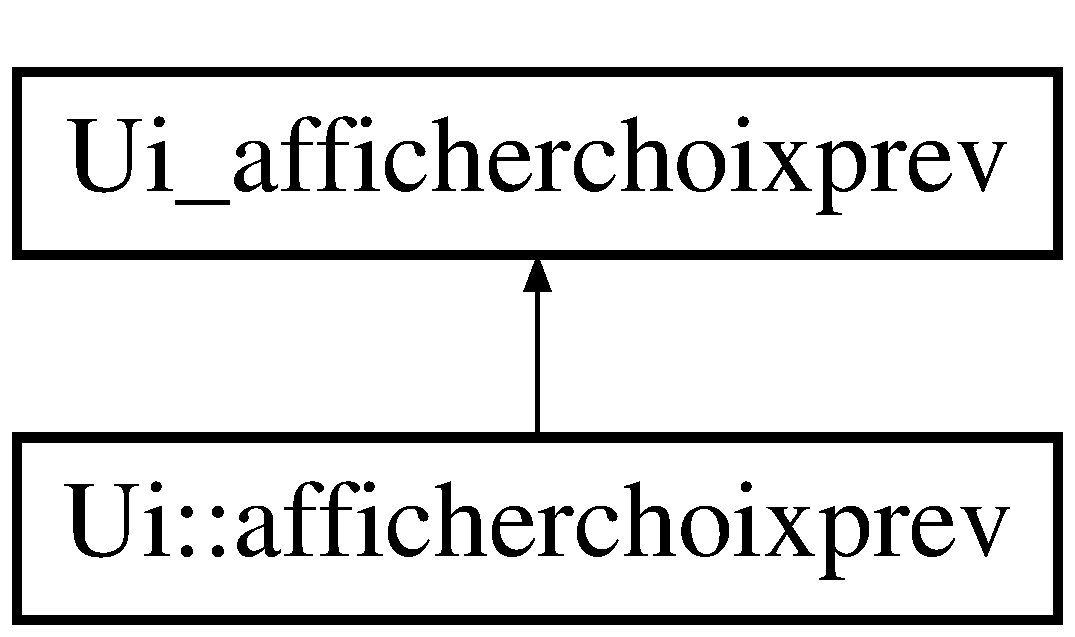
\includegraphics[height=2.000000cm]{class_ui__afficherchoixprev}
\end{center}
\end{figure}
\subsection*{Fonctions membres publiques}
\begin{DoxyCompactItemize}
\item 
\hypertarget{class_ui__afficherchoixprev_a4ce57f375bb3ce390d6a30b3dfb1df5b}{void {\bfseries setup\+Ui} (Q\+Widget $\ast$\hyperlink{classafficherchoixprev}{afficherchoixprev})}\label{class_ui__afficherchoixprev_a4ce57f375bb3ce390d6a30b3dfb1df5b}

\item 
\hypertarget{class_ui__afficherchoixprev_a78435987c98b93201a36d9dbe65b8f7c}{void {\bfseries retranslate\+Ui} (Q\+Widget $\ast$\hyperlink{classafficherchoixprev}{afficherchoixprev})}\label{class_ui__afficherchoixprev_a78435987c98b93201a36d9dbe65b8f7c}

\end{DoxyCompactItemize}
\subsection*{Attributs publics}
\begin{DoxyCompactItemize}
\item 
\hypertarget{class_ui__afficherchoixprev_ac6b05a5a980825d4cfac6563fb8d324c}{Q\+List\+Widget $\ast$ {\bfseries uv\+\_\+6}}\label{class_ui__afficherchoixprev_ac6b05a5a980825d4cfac6563fb8d324c}

\item 
\hypertarget{class_ui__afficherchoixprev_a8b22121c733404e0849914f589d872d1}{Q\+Frame $\ast$ {\bfseries line}}\label{class_ui__afficherchoixprev_a8b22121c733404e0849914f589d872d1}

\item 
\hypertarget{class_ui__afficherchoixprev_ab03590db10035bbe3ea1726e9d266014}{Q\+Label $\ast$ {\bfseries label\+\_\+7}}\label{class_ui__afficherchoixprev_ab03590db10035bbe3ea1726e9d266014}

\item 
\hypertarget{class_ui__afficherchoixprev_a0227d0da0daa6d8c57dfbe22b47d1421}{Q\+Label $\ast$ {\bfseries label\+\_\+8}}\label{class_ui__afficherchoixprev_a0227d0da0daa6d8c57dfbe22b47d1421}

\item 
\hypertarget{class_ui__afficherchoixprev_af24b698af1cbe0bad6ca9d1d2939ad48}{Q\+Frame $\ast$ {\bfseries line\+\_\+6}}\label{class_ui__afficherchoixprev_af24b698af1cbe0bad6ca9d1d2939ad48}

\item 
\hypertarget{class_ui__afficherchoixprev_a87bdc0304f1d357a43f7e813d6593d94}{Q\+Frame $\ast$ {\bfseries line\+\_\+8}}\label{class_ui__afficherchoixprev_a87bdc0304f1d357a43f7e813d6593d94}

\item 
\hypertarget{class_ui__afficherchoixprev_aef53551c97a335b5620645966a990103}{Q\+Label $\ast$ {\bfseries label\+\_\+10}}\label{class_ui__afficherchoixprev_aef53551c97a335b5620645966a990103}

\item 
\hypertarget{class_ui__afficherchoixprev_a9501efcf511e8d6afcc7dba1f609ede7}{Q\+List\+Widget $\ast$ {\bfseries uv\+\_\+1}}\label{class_ui__afficherchoixprev_a9501efcf511e8d6afcc7dba1f609ede7}

\item 
\hypertarget{class_ui__afficherchoixprev_ae7e6acc56dd966f7aa58c9ed4ff38f68}{Q\+List\+Widget $\ast$ {\bfseries uv\+\_\+3}}\label{class_ui__afficherchoixprev_ae7e6acc56dd966f7aa58c9ed4ff38f68}

\item 
\hypertarget{class_ui__afficherchoixprev_a8252cbb4c9822b676c97bfbf7dc74f74}{Q\+Label $\ast$ {\bfseries label\+\_\+5}}\label{class_ui__afficherchoixprev_a8252cbb4c9822b676c97bfbf7dc74f74}

\item 
\hypertarget{class_ui__afficherchoixprev_ac3cccbf7d880bc680b663c176ee045e6}{Q\+List\+Widget $\ast$ {\bfseries uv\+\_\+8}}\label{class_ui__afficherchoixprev_ac3cccbf7d880bc680b663c176ee045e6}

\item 
\hypertarget{class_ui__afficherchoixprev_a846903bc12d9476d6490835f47911743}{Q\+Label $\ast$ {\bfseries label\+\_\+6}}\label{class_ui__afficherchoixprev_a846903bc12d9476d6490835f47911743}

\item 
\hypertarget{class_ui__afficherchoixprev_ae723d677c3266fac0f950ddb394f812d}{Q\+Label $\ast$ {\bfseries label\+\_\+11}}\label{class_ui__afficherchoixprev_ae723d677c3266fac0f950ddb394f812d}

\item 
\hypertarget{class_ui__afficherchoixprev_a5fbfd3270e0a8fc0e737459fbf9e3909}{Q\+List\+Widget $\ast$ {\bfseries uv\+\_\+4}}\label{class_ui__afficherchoixprev_a5fbfd3270e0a8fc0e737459fbf9e3909}

\item 
\hypertarget{class_ui__afficherchoixprev_a1795e613f1b87955ccd1c1b7045d0b82}{Q\+Label $\ast$ {\bfseries label\+\_\+12}}\label{class_ui__afficherchoixprev_a1795e613f1b87955ccd1c1b7045d0b82}

\item 
\hypertarget{class_ui__afficherchoixprev_aec109dec69bd6e164898beab66d979c7}{Q\+Label $\ast$ {\bfseries label\+\_\+13}}\label{class_ui__afficherchoixprev_aec109dec69bd6e164898beab66d979c7}

\item 
\hypertarget{class_ui__afficherchoixprev_a65f9bf9f1846646d90a5f0b873d795ee}{Q\+Frame $\ast$ {\bfseries line\+\_\+2}}\label{class_ui__afficherchoixprev_a65f9bf9f1846646d90a5f0b873d795ee}

\item 
\hypertarget{class_ui__afficherchoixprev_a2879416a50ccc2f547783259a48fb0de}{Q\+Label $\ast$ {\bfseries label}}\label{class_ui__afficherchoixprev_a2879416a50ccc2f547783259a48fb0de}

\item 
\hypertarget{class_ui__afficherchoixprev_a52f09eb47e5fd7c2b7aa00b773a1bdca}{Q\+Label $\ast$ {\bfseries label\+\_\+2}}\label{class_ui__afficherchoixprev_a52f09eb47e5fd7c2b7aa00b773a1bdca}

\item 
\hypertarget{class_ui__afficherchoixprev_a70e620c66644a82a9ef608a57f611f01}{Q\+Label $\ast$ {\bfseries label\+\_\+9}}\label{class_ui__afficherchoixprev_a70e620c66644a82a9ef608a57f611f01}

\item 
\hypertarget{class_ui__afficherchoixprev_a5b34a9a3d5c5ff0cb229905bcbcf2c8b}{Q\+Frame $\ast$ {\bfseries line\+\_\+4}}\label{class_ui__afficherchoixprev_a5b34a9a3d5c5ff0cb229905bcbcf2c8b}

\item 
\hypertarget{class_ui__afficherchoixprev_a5bd9a8223c27150e8a8cc0ff24c7d00c}{Q\+Label $\ast$ {\bfseries label\+\_\+4}}\label{class_ui__afficherchoixprev_a5bd9a8223c27150e8a8cc0ff24c7d00c}

\item 
\hypertarget{class_ui__afficherchoixprev_ab245c221fae157936a63833e454b3d5f}{Q\+Frame $\ast$ {\bfseries line\+\_\+5}}\label{class_ui__afficherchoixprev_ab245c221fae157936a63833e454b3d5f}

\item 
\hypertarget{class_ui__afficherchoixprev_abda8fda8a1da91974f57aad57ddbea2b}{Q\+Label $\ast$ {\bfseries label\+\_\+3}}\label{class_ui__afficherchoixprev_abda8fda8a1da91974f57aad57ddbea2b}

\item 
\hypertarget{class_ui__afficherchoixprev_a2be4f30a4da5408b9a9cea02a42a3c84}{Q\+Label $\ast$ {\bfseries label\+\_\+14}}\label{class_ui__afficherchoixprev_a2be4f30a4da5408b9a9cea02a42a3c84}

\item 
\hypertarget{class_ui__afficherchoixprev_a8b115b8c98b279d78fb3ad1040c9f6d9}{Q\+List\+Widget $\ast$ {\bfseries uv\+\_\+2}}\label{class_ui__afficherchoixprev_a8b115b8c98b279d78fb3ad1040c9f6d9}

\item 
\hypertarget{class_ui__afficherchoixprev_a2d53964dc35a4645face3abd1e711ca2}{Q\+List\+Widget $\ast$ {\bfseries uv\+\_\+5}}\label{class_ui__afficherchoixprev_a2d53964dc35a4645face3abd1e711ca2}

\item 
\hypertarget{class_ui__afficherchoixprev_a5fba9fe523307277a3b3e9cbba268b51}{Q\+List\+Widget $\ast$ {\bfseries uv\+\_\+7}}\label{class_ui__afficherchoixprev_a5fba9fe523307277a3b3e9cbba268b51}

\item 
\hypertarget{class_ui__afficherchoixprev_af8701f530cc1d58cd59a5a8fef73a1d9}{Q\+Frame $\ast$ {\bfseries line\+\_\+3}}\label{class_ui__afficherchoixprev_af8701f530cc1d58cd59a5a8fef73a1d9}

\end{DoxyCompactItemize}


La documentation de cette classe a été générée à partir du fichier suivant \+:\begin{DoxyCompactItemize}
\item 
ui\+\_\+afficherchoixprev.\+h\end{DoxyCompactItemize}

\hypertarget{class_ui__detailuv}{\section{Référence de la classe Ui\+\_\+detailuv}
\label{class_ui__detailuv}\index{Ui\+\_\+detailuv@{Ui\+\_\+detailuv}}
}
Graphe d'héritage de Ui\+\_\+detailuv\+:\begin{figure}[H]
\begin{center}
\leavevmode
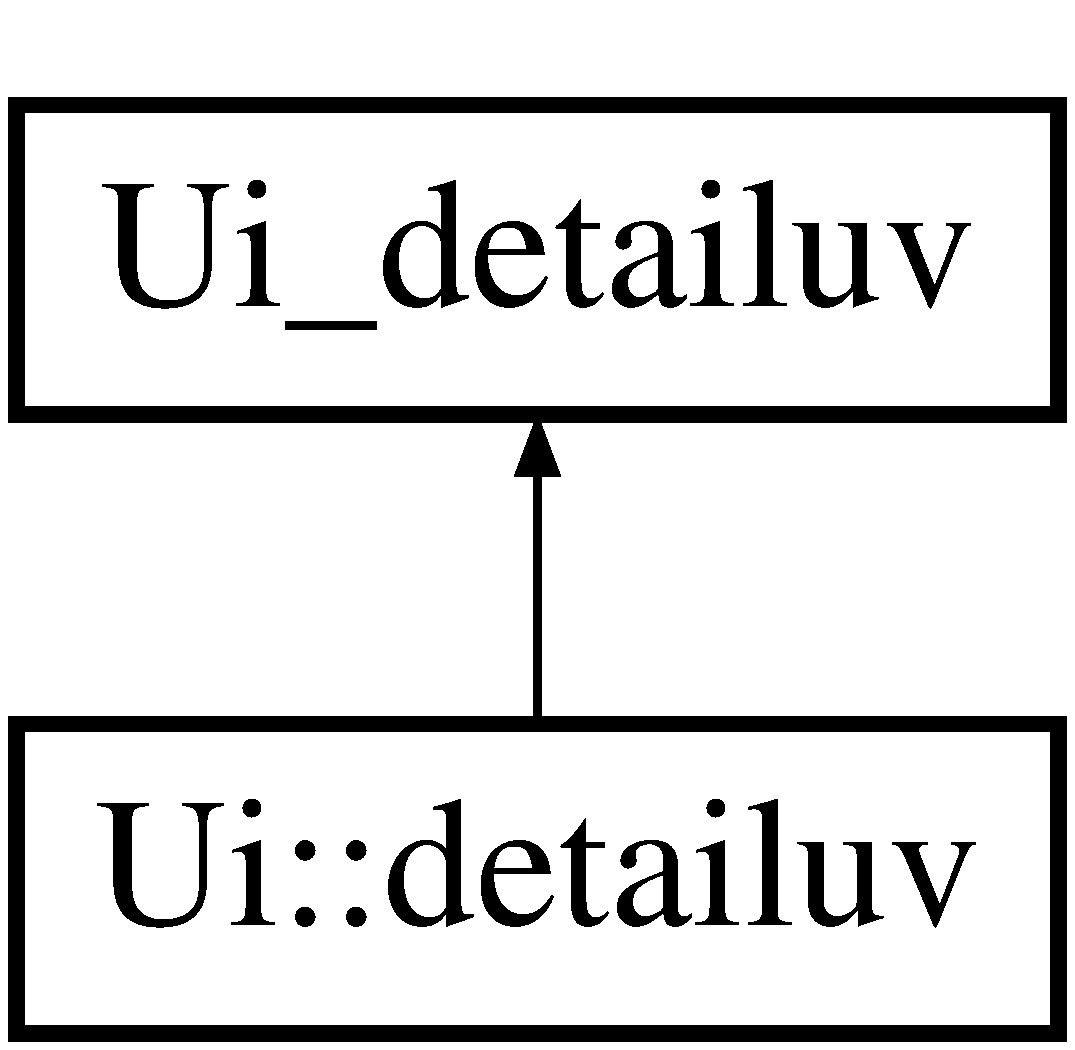
\includegraphics[height=2.000000cm]{class_ui__detailuv}
\end{center}
\end{figure}
\subsection*{Fonctions membres publiques}
\begin{DoxyCompactItemize}
\item 
\hypertarget{class_ui__detailuv_ac10a5ecc791bc18309ffda5d67470e40}{void {\bfseries setup\+Ui} (Q\+Widget $\ast$\hyperlink{classdetailuv}{detailuv})}\label{class_ui__detailuv_ac10a5ecc791bc18309ffda5d67470e40}

\item 
\hypertarget{class_ui__detailuv_a2b4b9e96634a500527d26c3a501bfd33}{void {\bfseries retranslate\+Ui} (Q\+Widget $\ast$\hyperlink{classdetailuv}{detailuv})}\label{class_ui__detailuv_a2b4b9e96634a500527d26c3a501bfd33}

\end{DoxyCompactItemize}
\subsection*{Attributs publics}
\begin{DoxyCompactItemize}
\item 
\hypertarget{class_ui__detailuv_a2ea14ca970804051281aed9e8f3d5718}{Q\+Label $\ast$ {\bfseries titre}}\label{class_ui__detailuv_a2ea14ca970804051281aed9e8f3d5718}

\item 
\hypertarget{class_ui__detailuv_ac582115f229620099ac17dc4938711b0}{Q\+Label $\ast$ {\bfseries codetitre}}\label{class_ui__detailuv_ac582115f229620099ac17dc4938711b0}

\item 
\hypertarget{class_ui__detailuv_a37fcde4804264386d9cba8c58361eae1}{Q\+Label $\ast$ {\bfseries label}}\label{class_ui__detailuv_a37fcde4804264386d9cba8c58361eae1}

\item 
\hypertarget{class_ui__detailuv_a9c24372971b586b443678bcc708e6f5a}{Q\+Text\+Browser $\ast$ {\bfseries text\+Browser}}\label{class_ui__detailuv_a9c24372971b586b443678bcc708e6f5a}

\item 
\hypertarget{class_ui__detailuv_a1c7a4132a6949d6dff1aa700e9d51302}{Q\+Label $\ast$ {\bfseries label\+\_\+dispo}}\label{class_ui__detailuv_a1c7a4132a6949d6dff1aa700e9d51302}

\item 
\hypertarget{class_ui__detailuv_a4855d8d6473d696c752097918082ce11}{Q\+List\+View $\ast$ {\bfseries list\+\_\+dispo}}\label{class_ui__detailuv_a4855d8d6473d696c752097918082ce11}

\end{DoxyCompactItemize}


La documentation de cette classe a été générée à partir du fichier suivant \+:\begin{DoxyCompactItemize}
\item 
ui\+\_\+detailuv.\+h\end{DoxyCompactItemize}

\hypertarget{class_ui__fenetreplus}{\section{Référence de la classe Ui\+\_\+fenetreplus}
\label{class_ui__fenetreplus}\index{Ui\+\_\+fenetreplus@{Ui\+\_\+fenetreplus}}
}
Graphe d'héritage de Ui\+\_\+fenetreplus\+:\begin{figure}[H]
\begin{center}
\leavevmode
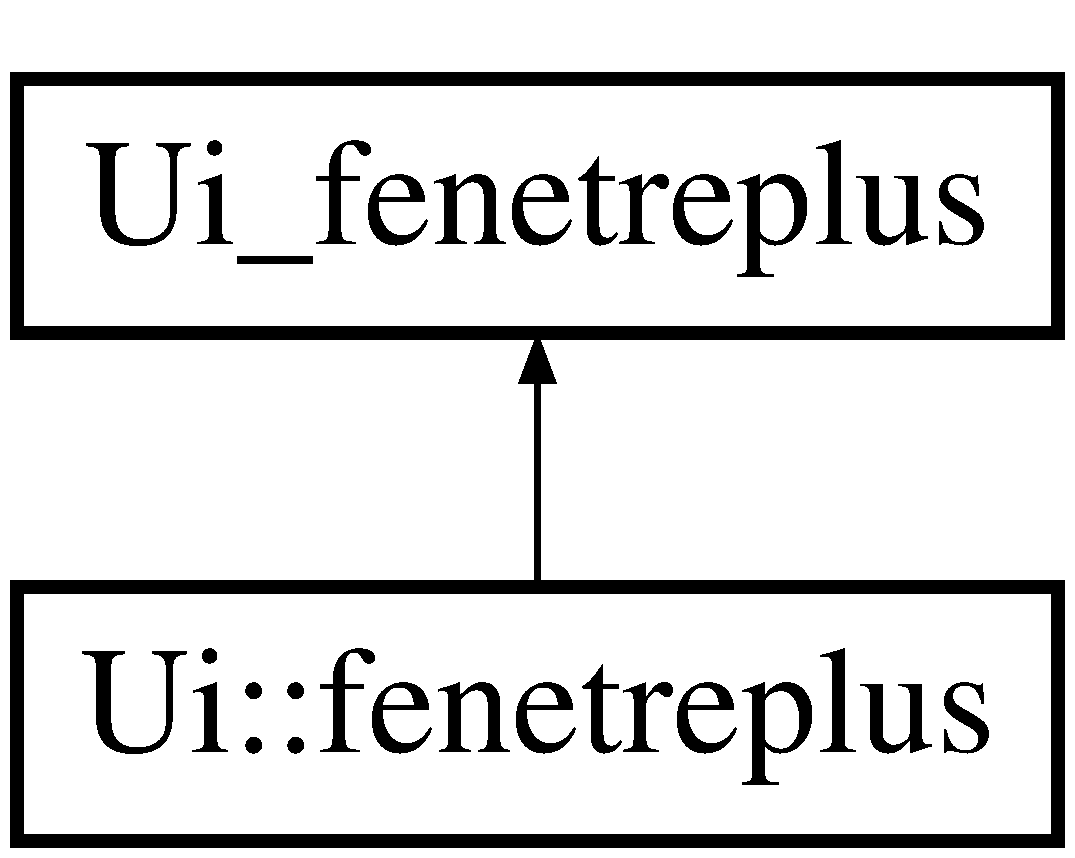
\includegraphics[height=2.000000cm]{class_ui__fenetreplus}
\end{center}
\end{figure}
\subsection*{Fonctions membres publiques}
\begin{DoxyCompactItemize}
\item 
\hypertarget{class_ui__fenetreplus_ad9ec92335e0e91902dcd1315dea84277}{void {\bfseries setup\+Ui} (Q\+Widget $\ast$\hyperlink{classfenetreplus}{fenetreplus})}\label{class_ui__fenetreplus_ad9ec92335e0e91902dcd1315dea84277}

\item 
\hypertarget{class_ui__fenetreplus_abbb24df954d24d1b5bea37d4a643bc85}{void {\bfseries retranslate\+Ui} (Q\+Widget $\ast$\hyperlink{classfenetreplus}{fenetreplus})}\label{class_ui__fenetreplus_abbb24df954d24d1b5bea37d4a643bc85}

\end{DoxyCompactItemize}
\subsection*{Attributs publics}
\begin{DoxyCompactItemize}
\item 
\hypertarget{class_ui__fenetreplus_a2c4285d9a61770e3c2e9f757baf8b69b}{Q\+Command\+Link\+Button $\ast$ {\bfseries command\+Link\+Button}}\label{class_ui__fenetreplus_a2c4285d9a61770e3c2e9f757baf8b69b}

\end{DoxyCompactItemize}


La documentation de cette classe a été générée à partir du fichier suivant \+:\begin{DoxyCompactItemize}
\item 
ui\+\_\+fenetreplus.\+h\end{DoxyCompactItemize}

\hypertarget{class_ui___inscription}{\section{Référence de la classe Ui\+\_\+\+Inscription}
\label{class_ui___inscription}\index{Ui\+\_\+\+Inscription@{Ui\+\_\+\+Inscription}}
}
Graphe d'héritage de Ui\+\_\+\+Inscription\+:\begin{figure}[H]
\begin{center}
\leavevmode
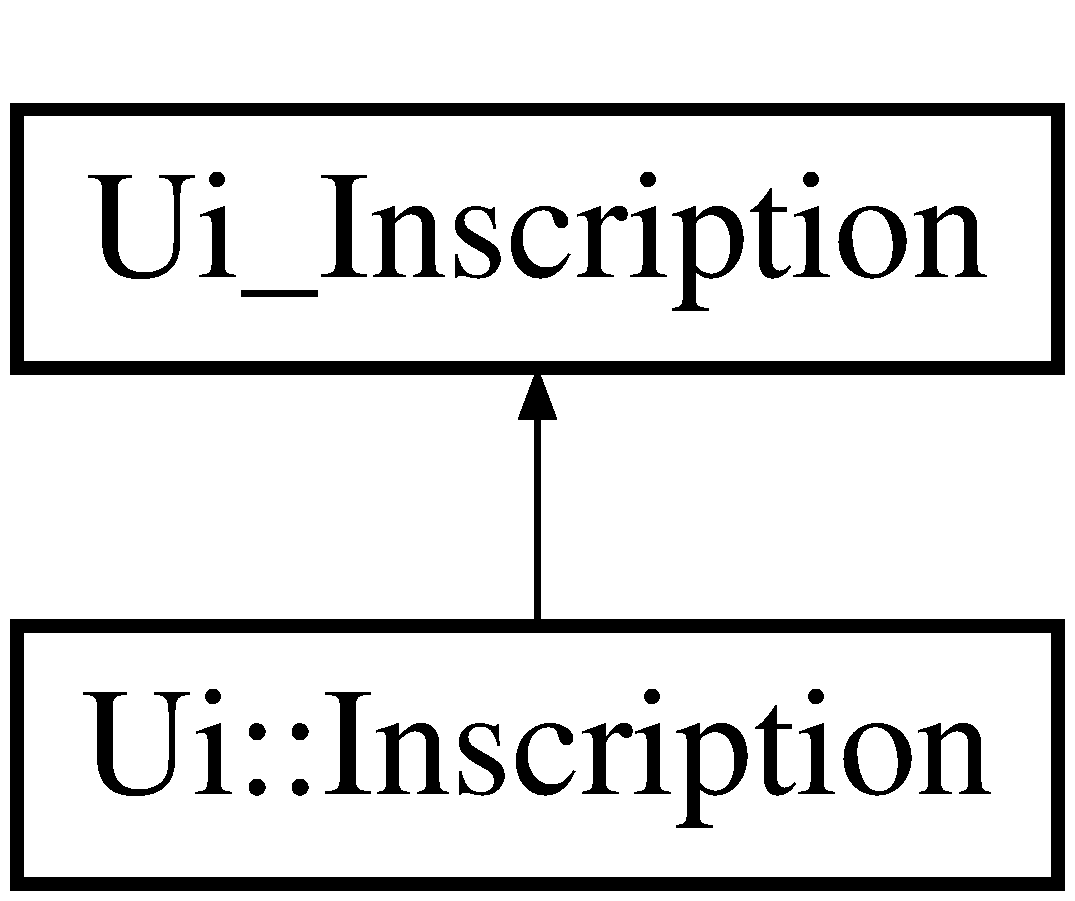
\includegraphics[height=2.000000cm]{class_ui___inscription}
\end{center}
\end{figure}
\subsection*{Fonctions membres publiques}
\begin{DoxyCompactItemize}
\item 
\hypertarget{class_ui___inscription_ae761c4d04f372cc6720601d2dec0f6b5}{void {\bfseries setup\+Ui} (Q\+Dialog $\ast$\hyperlink{class_inscription}{Inscription})}\label{class_ui___inscription_ae761c4d04f372cc6720601d2dec0f6b5}

\item 
\hypertarget{class_ui___inscription_a238a9407e2696e57733e912f4119dbea}{void {\bfseries retranslate\+Ui} (Q\+Dialog $\ast$\hyperlink{class_inscription}{Inscription})}\label{class_ui___inscription_a238a9407e2696e57733e912f4119dbea}

\end{DoxyCompactItemize}
\subsection*{Attributs publics}
\begin{DoxyCompactItemize}
\item 
\hypertarget{class_ui___inscription_a5b6a0eb92785d35fc88c6caebb7edb9f}{Q\+Label $\ast$ {\bfseries label\+\_\+login}}\label{class_ui___inscription_a5b6a0eb92785d35fc88c6caebb7edb9f}

\item 
\hypertarget{class_ui___inscription_a6b0427037d4bc09dbea78cb60bd5e7e8}{Q\+Label $\ast$ {\bfseries label\+\_\+nom}}\label{class_ui___inscription_a6b0427037d4bc09dbea78cb60bd5e7e8}

\item 
\hypertarget{class_ui___inscription_a85182f29f6159f1d33dd7546cada0069}{Q\+Label $\ast$ {\bfseries label\+\_\+prenom}}\label{class_ui___inscription_a85182f29f6159f1d33dd7546cada0069}

\item 
\hypertarget{class_ui___inscription_a7052a73fb2b4d5bc6f42f4d49963d9b2}{Q\+Label $\ast$ {\bfseries label\+\_\+mdp1}}\label{class_ui___inscription_a7052a73fb2b4d5bc6f42f4d49963d9b2}

\item 
\hypertarget{class_ui___inscription_a6552764d44e15895216025edac1369b2}{Q\+Label $\ast$ {\bfseries label\+\_\+mdp2}}\label{class_ui___inscription_a6552764d44e15895216025edac1369b2}

\item 
\hypertarget{class_ui___inscription_ad19889e455c84c6267ed520a50fa33e4}{Q\+Label $\ast$ {\bfseries label\+\_\+sexe}}\label{class_ui___inscription_ad19889e455c84c6267ed520a50fa33e4}

\item 
\hypertarget{class_ui___inscription_abdc177bfde089af67d98923ae384c82d}{Q\+Line\+Edit $\ast$ {\bfseries input\+\_\+login}}\label{class_ui___inscription_abdc177bfde089af67d98923ae384c82d}

\item 
\hypertarget{class_ui___inscription_a1602d15a06923ffdacdace78d066c728}{Q\+Line\+Edit $\ast$ {\bfseries input\+\_\+nom}}\label{class_ui___inscription_a1602d15a06923ffdacdace78d066c728}

\item 
\hypertarget{class_ui___inscription_a3b437f526be046519bb7eaad0b79528c}{Q\+Line\+Edit $\ast$ {\bfseries input\+\_\+prenom}}\label{class_ui___inscription_a3b437f526be046519bb7eaad0b79528c}

\item 
\hypertarget{class_ui___inscription_a9ebb8ea10beba00784b6ea3f8d6306af}{Q\+Line\+Edit $\ast$ {\bfseries input\+\_\+mdp}}\label{class_ui___inscription_a9ebb8ea10beba00784b6ea3f8d6306af}

\item 
\hypertarget{class_ui___inscription_a1c52bf60a8441773c95a2136e7b9ad1b}{Q\+Line\+Edit $\ast$ {\bfseries input\+\_\+mdp2}}\label{class_ui___inscription_a1c52bf60a8441773c95a2136e7b9ad1b}

\item 
\hypertarget{class_ui___inscription_aacb81fb622d07ae64c192fb121b66582}{Q\+Label $\ast$ {\bfseries label\+\_\+titre}}\label{class_ui___inscription_aacb81fb622d07ae64c192fb121b66582}

\item 
\hypertarget{class_ui___inscription_a5044b8606f21934011ba0df90817297b}{Q\+Combo\+Box $\ast$ {\bfseries combo\+Box}}\label{class_ui___inscription_a5044b8606f21934011ba0df90817297b}

\item 
\hypertarget{class_ui___inscription_a59dbcf2ada7833d8c36b64a1fc995582}{Q\+Push\+Button $\ast$ {\bfseries valider}}\label{class_ui___inscription_a59dbcf2ada7833d8c36b64a1fc995582}

\item 
\hypertarget{class_ui___inscription_a4a3fbf34812b5d6c48ac8d34b66a84c1}{Q\+Label $\ast$ {\bfseries label\+\_\+email}}\label{class_ui___inscription_a4a3fbf34812b5d6c48ac8d34b66a84c1}

\item 
\hypertarget{class_ui___inscription_a5c644d872ccddc1f1ea1f52f7bd0cfe4}{Q\+Line\+Edit $\ast$ {\bfseries input\+\_\+email}}\label{class_ui___inscription_a5c644d872ccddc1f1ea1f52f7bd0cfe4}

\item 
\hypertarget{class_ui___inscription_a29aea056f11b80b0e175b416181337bd}{Q\+Label $\ast$ {\bfseries label\+\_\+datenaiss}}\label{class_ui___inscription_a29aea056f11b80b0e175b416181337bd}

\item 
\hypertarget{class_ui___inscription_ad0597359d0a9f937e36ccd1313b94835}{Q\+Line\+Edit $\ast$ {\bfseries input\+\_\+date\+\_\+naiss}}\label{class_ui___inscription_ad0597359d0a9f937e36ccd1313b94835}

\item 
\hypertarget{class_ui___inscription_ab8845f7f43c5f723b97972f352b09f57}{Q\+Combo\+Box $\ast$ {\bfseries combo\+Box\+\_\+cursus}}\label{class_ui___inscription_ab8845f7f43c5f723b97972f352b09f57}

\item 
\hypertarget{class_ui___inscription_a78d434455289bba5e01201f2f5603cf6}{Q\+Label $\ast$ {\bfseries label\+\_\+cursus}}\label{class_ui___inscription_a78d434455289bba5e01201f2f5603cf6}

\item 
\hypertarget{class_ui___inscription_af948b1cbf1fdeceb025142a7d9d30c3f}{Q\+Combo\+Box $\ast$ {\bfseries combo\+Box\+\_\+branche}}\label{class_ui___inscription_af948b1cbf1fdeceb025142a7d9d30c3f}

\item 
\hypertarget{class_ui___inscription_a82434ae5620ed068723a5af25b48788f}{Q\+Label $\ast$ {\bfseries label\+\_\+branche}}\label{class_ui___inscription_a82434ae5620ed068723a5af25b48788f}

\item 
\hypertarget{class_ui___inscription_a76755d83bd82d04da3b0ac4f528f58b1}{Q\+Combo\+Box $\ast$ {\bfseries combo\+Box\+\_\+filiere}}\label{class_ui___inscription_a76755d83bd82d04da3b0ac4f528f58b1}

\item 
\hypertarget{class_ui___inscription_a8352af532dd880915bdffee680950cb3}{Q\+Label $\ast$ {\bfseries label\+\_\+filiere}}\label{class_ui___inscription_a8352af532dd880915bdffee680950cb3}

\item 
\hypertarget{class_ui___inscription_a8c3f31f68f307b7827f7653c99cbe155}{Q\+Combo\+Box $\ast$ {\bfseries combo\+Box\+\_\+semestre}}\label{class_ui___inscription_a8c3f31f68f307b7827f7653c99cbe155}

\item 
\hypertarget{class_ui___inscription_a7644a994ad9a3f36bb739f298ce4970f}{Q\+Label $\ast$ {\bfseries label\+\_\+semestre}}\label{class_ui___inscription_a7644a994ad9a3f36bb739f298ce4970f}

\item 
\hypertarget{class_ui___inscription_a0e0cb171f2ff3b36dd00357e064a0109}{Q\+Label $\ast$ {\bfseries label}}\label{class_ui___inscription_a0e0cb171f2ff3b36dd00357e064a0109}

\end{DoxyCompactItemize}


La documentation de cette classe a été générée à partir du fichier suivant \+:\begin{DoxyCompactItemize}
\item 
ui\+\_\+inscription.\+h\end{DoxyCompactItemize}

\hypertarget{class_ui___insert_uv}{\section{Référence de la classe Ui\+\_\+\+Insert\+Uv}
\label{class_ui___insert_uv}\index{Ui\+\_\+\+Insert\+Uv@{Ui\+\_\+\+Insert\+Uv}}
}
Graphe d'héritage de Ui\+\_\+\+Insert\+Uv\+:\begin{figure}[H]
\begin{center}
\leavevmode
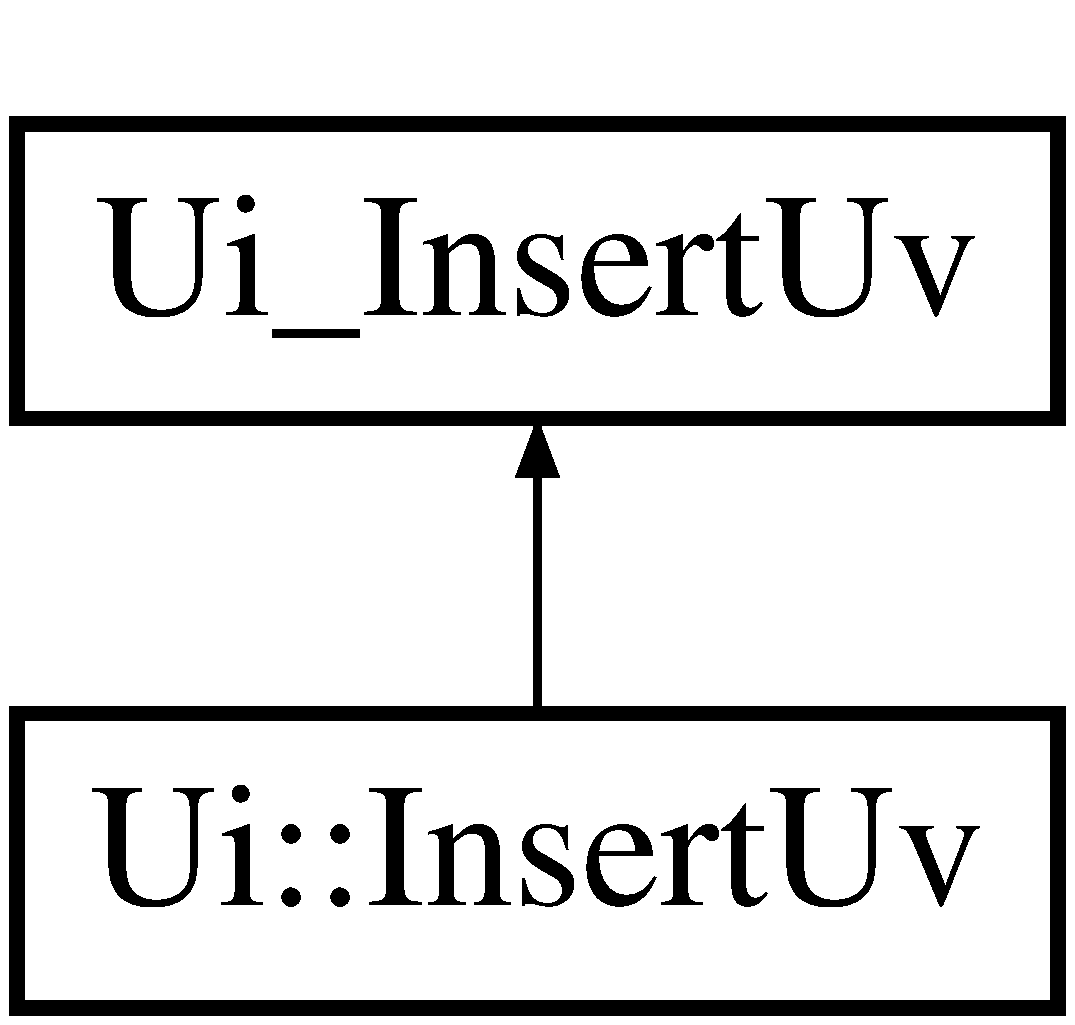
\includegraphics[height=2.000000cm]{class_ui___insert_uv}
\end{center}
\end{figure}
\subsection*{Fonctions membres publiques}
\begin{DoxyCompactItemize}
\item 
\hypertarget{class_ui___insert_uv_a08460e0d2fbbd5d2a67913e3c2fbc1c9}{void {\bfseries setup\+Ui} (Q\+Widget $\ast$\hyperlink{class_insert_uv}{Insert\+Uv})}\label{class_ui___insert_uv_a08460e0d2fbbd5d2a67913e3c2fbc1c9}

\item 
\hypertarget{class_ui___insert_uv_a1c13bea0dac65e742cc743e0e7eeb698}{void {\bfseries retranslate\+Ui} (Q\+Widget $\ast$\hyperlink{class_insert_uv}{Insert\+Uv})}\label{class_ui___insert_uv_a1c13bea0dac65e742cc743e0e7eeb698}

\end{DoxyCompactItemize}
\subsection*{Attributs publics}
\begin{DoxyCompactItemize}
\item 
\hypertarget{class_ui___insert_uv_a5ba283a28c569e03719d6813392a711c}{Q\+Label $\ast$ {\bfseries label\+\_\+code}}\label{class_ui___insert_uv_a5ba283a28c569e03719d6813392a711c}

\item 
\hypertarget{class_ui___insert_uv_abb78ad9220e9a1c0460a7e18c6cec4a2}{Q\+Line\+Edit $\ast$ {\bfseries input\+\_\+code}}\label{class_ui___insert_uv_abb78ad9220e9a1c0460a7e18c6cec4a2}

\item 
\hypertarget{class_ui___insert_uv_ac604b350abc147ca0d03c1346269064a}{Q\+Label $\ast$ {\bfseries label\+\_\+2}}\label{class_ui___insert_uv_ac604b350abc147ca0d03c1346269064a}

\item 
\hypertarget{class_ui___insert_uv_a530092c5a4143dd31a215ef3116f6578}{Q\+Label $\ast$ {\bfseries label\+\_\+cate}}\label{class_ui___insert_uv_a530092c5a4143dd31a215ef3116f6578}

\item 
\hypertarget{class_ui___insert_uv_a6efd74c426a38a164298326028c401ce}{Q\+Check\+Box $\ast$ {\bfseries check\+Box\+\_\+cs1}}\label{class_ui___insert_uv_a6efd74c426a38a164298326028c401ce}

\item 
\hypertarget{class_ui___insert_uv_aed57598a20320fcb383d52b2189e8543}{Q\+Check\+Box $\ast$ {\bfseries check\+Box\+\_\+tm2}}\label{class_ui___insert_uv_aed57598a20320fcb383d52b2189e8543}

\item 
\hypertarget{class_ui___insert_uv_afbb344c4326fc7f3aac9226b01d7c09a}{Q\+Check\+Box $\ast$ {\bfseries check\+Box\+\_\+\+\_\+tsh3}}\label{class_ui___insert_uv_afbb344c4326fc7f3aac9226b01d7c09a}

\item 
\hypertarget{class_ui___insert_uv_ae76bf1d37d4c77fae164fac42ffb24d4}{Q\+Check\+Box $\ast$ {\bfseries check\+Box\+\_\+sp4}}\label{class_ui___insert_uv_ae76bf1d37d4c77fae164fac42ffb24d4}

\item 
\hypertarget{class_ui___insert_uv_a5c9615a5a668cc24d61856395bb22e01}{Q\+Label $\ast$ {\bfseries label\+\_\+cate\+\_\+2}}\label{class_ui___insert_uv_a5c9615a5a668cc24d61856395bb22e01}

\item 
\hypertarget{class_ui___insert_uv_a1801dcec22580062a7eeb61a76a9b43a}{Q\+Check\+Box $\ast$ {\bfseries check\+Box\+\_\+ingenieur}}\label{class_ui___insert_uv_a1801dcec22580062a7eeb61a76a9b43a}

\item 
\hypertarget{class_ui___insert_uv_a9b54ea880e1d61d165223ec792ded42d}{Q\+Check\+Box $\ast$ {\bfseries check\+Box\+\_\+master}}\label{class_ui___insert_uv_a9b54ea880e1d61d165223ec792ded42d}

\item 
\hypertarget{class_ui___insert_uv_a25556ca38cbd94eeb132317961f89706}{Q\+Label $\ast$ {\bfseries label\+\_\+cate\+\_\+3}}\label{class_ui___insert_uv_a25556ca38cbd94eeb132317961f89706}

\item 
\hypertarget{class_ui___insert_uv_ac2d6cb05974b9c403bb2a2483c90fde6}{Q\+Check\+Box $\ast$ {\bfseries check\+Box\+\_\+general}}\label{class_ui___insert_uv_ac2d6cb05974b9c403bb2a2483c90fde6}

\item 
\hypertarget{class_ui___insert_uv_ac676eadb62bae93a4432cc7e8ff5e9c9}{Q\+Check\+Box $\ast$ {\bfseries check\+Box\+\_\+tm\+\_\+1}}\label{class_ui___insert_uv_ac676eadb62bae93a4432cc7e8ff5e9c9}

\item 
\hypertarget{class_ui___insert_uv_ad33b743be5ddb536afa332cdfa6fe2f6}{Q\+Check\+Box $\ast$ {\bfseries check\+Box\+\_\+\+\_\+tsh2}}\label{class_ui___insert_uv_ad33b743be5ddb536afa332cdfa6fe2f6}

\item 
\hypertarget{class_ui___insert_uv_a140af06a71463f85febef8b812ba131e}{Q\+Check\+Box $\ast$ {\bfseries check\+Box\+\_\+sp3}}\label{class_ui___insert_uv_a140af06a71463f85febef8b812ba131e}

\item 
\hypertarget{class_ui___insert_uv_abc4841f50f493b135f294416d58afec5}{Q\+Check\+Box $\ast$ {\bfseries check\+Box\+\_\+cs4}}\label{class_ui___insert_uv_abc4841f50f493b135f294416d58afec5}

\item 
\hypertarget{class_ui___insert_uv_a0b8acd6415e20e36bc4f0a6b2e5fb3e0}{Q\+Check\+Box $\ast$ {\bfseries check\+Box\+\_\+\+\_\+tsh\+\_\+1}}\label{class_ui___insert_uv_a0b8acd6415e20e36bc4f0a6b2e5fb3e0}

\item 
\hypertarget{class_ui___insert_uv_a7a3010d70992ddead088d136322cde27}{Q\+Check\+Box $\ast$ {\bfseries check\+Box\+\_\+sp2}}\label{class_ui___insert_uv_a7a3010d70992ddead088d136322cde27}

\item 
\hypertarget{class_ui___insert_uv_a20c599afdf8367b000f863ba0337be40}{Q\+Check\+Box $\ast$ {\bfseries check\+Box\+\_\+cs3}}\label{class_ui___insert_uv_a20c599afdf8367b000f863ba0337be40}

\item 
\hypertarget{class_ui___insert_uv_a0e0f91612f0478f05d2e06594acadee9}{Q\+Check\+Box $\ast$ {\bfseries check\+Box\+\_\+tm4}}\label{class_ui___insert_uv_a0e0f91612f0478f05d2e06594acadee9}

\item 
\hypertarget{class_ui___insert_uv_a3a6b62efe954940c5d16cea391bb5861}{Q\+Check\+Box $\ast$ {\bfseries check\+Box\+\_\+sp\+\_\+1}}\label{class_ui___insert_uv_a3a6b62efe954940c5d16cea391bb5861}

\item 
\hypertarget{class_ui___insert_uv_ae1503b786fef0a7ed9c1173a75103dbc}{Q\+Check\+Box $\ast$ {\bfseries check\+Box\+\_\+tm3}}\label{class_ui___insert_uv_ae1503b786fef0a7ed9c1173a75103dbc}

\item 
\hypertarget{class_ui___insert_uv_ae371929272ee164bd18343acf595b3f6}{Q\+Check\+Box $\ast$ {\bfseries check\+Box\+\_\+\+\_\+tsh4}}\label{class_ui___insert_uv_ae371929272ee164bd18343acf595b3f6}

\item 
\hypertarget{class_ui___insert_uv_ac65bdab475f3ae3d0e9b6e9d2c520922}{Q\+Check\+Box $\ast$ {\bfseries check\+Box\+\_\+cs2}}\label{class_ui___insert_uv_ac65bdab475f3ae3d0e9b6e9d2c520922}

\item 
\hypertarget{class_ui___insert_uv_ac540ed0f21a5398ff8f2239c9605ecca}{Q\+Label $\ast$ {\bfseries label\+\_\+code\+\_\+2}}\label{class_ui___insert_uv_ac540ed0f21a5398ff8f2239c9605ecca}

\item 
\hypertarget{class_ui___insert_uv_af7f29add537968572fe7e496e05982ed}{Q\+Label $\ast$ {\bfseries label\+\_\+code\+\_\+3}}\label{class_ui___insert_uv_af7f29add537968572fe7e496e05982ed}

\item 
\hypertarget{class_ui___insert_uv_aa1a33d96ab3ccd35968c66d6d3a25fd3}{Q\+Label $\ast$ {\bfseries label\+\_\+code\+\_\+4}}\label{class_ui___insert_uv_aa1a33d96ab3ccd35968c66d6d3a25fd3}

\item 
\hypertarget{class_ui___insert_uv_a6c130ae49e7482a419e0c67cffdaef07}{Q\+Label $\ast$ {\bfseries label\+\_\+code\+\_\+5}}\label{class_ui___insert_uv_a6c130ae49e7482a419e0c67cffdaef07}

\item 
\hypertarget{class_ui___insert_uv_ad4fb01f57b471dba126bb60ea3aaa800}{Q\+Frame $\ast$ {\bfseries line}}\label{class_ui___insert_uv_ad4fb01f57b471dba126bb60ea3aaa800}

\item 
\hypertarget{class_ui___insert_uv_acc5eec634575f66583bc2da69f48a40f}{Q\+Frame $\ast$ {\bfseries line\+\_\+2}}\label{class_ui___insert_uv_acc5eec634575f66583bc2da69f48a40f}

\item 
\hypertarget{class_ui___insert_uv_abb3578c50433b931737d4f07230359a0}{Q\+Frame $\ast$ {\bfseries line\+\_\+3}}\label{class_ui___insert_uv_abb3578c50433b931737d4f07230359a0}

\item 
\hypertarget{class_ui___insert_uv_ae4fcc882ad1227786f5943b007e60aa4}{Q\+Spin\+Box $\ast$ {\bfseries credit\+\_\+cs1}}\label{class_ui___insert_uv_ae4fcc882ad1227786f5943b007e60aa4}

\item 
\hypertarget{class_ui___insert_uv_aa0455658734a420cc0d4cca226025f1d}{Q\+Spin\+Box $\ast$ {\bfseries credit\+\_\+tm1}}\label{class_ui___insert_uv_aa0455658734a420cc0d4cca226025f1d}

\item 
\hypertarget{class_ui___insert_uv_a206cd398462b81f061f86f3f6e20b1b1}{Q\+Spin\+Box $\ast$ {\bfseries credit\+\_\+tsh1}}\label{class_ui___insert_uv_a206cd398462b81f061f86f3f6e20b1b1}

\item 
\hypertarget{class_ui___insert_uv_a7d0ca67f94ee8a4e24d002efe2930484}{Q\+Spin\+Box $\ast$ {\bfseries credit\+\_\+sp1}}\label{class_ui___insert_uv_a7d0ca67f94ee8a4e24d002efe2930484}

\item 
\hypertarget{class_ui___insert_uv_a16f600b61908d571148c88dbbc8e3da7}{Q\+Spin\+Box $\ast$ {\bfseries credit\+\_\+sp1\+\_\+2}}\label{class_ui___insert_uv_a16f600b61908d571148c88dbbc8e3da7}

\item 
\hypertarget{class_ui___insert_uv_a68999f499b1afce0202e009d4b49a1c9}{Q\+Spin\+Box $\ast$ {\bfseries credit\+\_\+sp2}}\label{class_ui___insert_uv_a68999f499b1afce0202e009d4b49a1c9}

\item 
\hypertarget{class_ui___insert_uv_a4fd2a4e4ebc7d099f749ce1594695d32}{Q\+Spin\+Box $\ast$ {\bfseries credit\+\_\+tsh2}}\label{class_ui___insert_uv_a4fd2a4e4ebc7d099f749ce1594695d32}

\item 
\hypertarget{class_ui___insert_uv_a2bf3690e2d1ff660be10607a60990220}{Q\+Spin\+Box $\ast$ {\bfseries credit\+\_\+tm2}}\label{class_ui___insert_uv_a2bf3690e2d1ff660be10607a60990220}

\item 
\hypertarget{class_ui___insert_uv_afce6f9bb4cee1607fef3bed885df13bd}{Q\+Spin\+Box $\ast$ {\bfseries credit\+\_\+sp3}}\label{class_ui___insert_uv_afce6f9bb4cee1607fef3bed885df13bd}

\item 
\hypertarget{class_ui___insert_uv_a4b846e4a4423219eeb271ab146abab8d}{Q\+Spin\+Box $\ast$ {\bfseries credit\+\_\+tm3}}\label{class_ui___insert_uv_a4b846e4a4423219eeb271ab146abab8d}

\item 
\hypertarget{class_ui___insert_uv_a110cfd687f3f8b5c1f54f956bca1b12e}{Q\+Spin\+Box $\ast$ {\bfseries credit\+\_\+tsh3}}\label{class_ui___insert_uv_a110cfd687f3f8b5c1f54f956bca1b12e}

\item 
\hypertarget{class_ui___insert_uv_a68d7cf9a2bc6ff5a4bc8beda01520b30}{Q\+Spin\+Box $\ast$ {\bfseries credit\+\_\+cs3}}\label{class_ui___insert_uv_a68d7cf9a2bc6ff5a4bc8beda01520b30}

\item 
\hypertarget{class_ui___insert_uv_a4c70160ffe1b0644850392f18f774080}{Q\+Spin\+Box $\ast$ {\bfseries credit\+\_\+tm4}}\label{class_ui___insert_uv_a4c70160ffe1b0644850392f18f774080}

\item 
\hypertarget{class_ui___insert_uv_a5d9eccf2c9b211a21b6f97e7b26bb097}{Q\+Spin\+Box $\ast$ {\bfseries credit\+\_\+cs4}}\label{class_ui___insert_uv_a5d9eccf2c9b211a21b6f97e7b26bb097}

\item 
\hypertarget{class_ui___insert_uv_a9437d3cd71137d8c1769d7fd8e32b1e9}{Q\+Spin\+Box $\ast$ {\bfseries credit\+\_\+sp4}}\label{class_ui___insert_uv_a9437d3cd71137d8c1769d7fd8e32b1e9}

\item 
\hypertarget{class_ui___insert_uv_a418bdc7aeb157c0ce709d0dd91cf507a}{Q\+Spin\+Box $\ast$ {\bfseries credit\+\_\+tsh4}}\label{class_ui___insert_uv_a418bdc7aeb157c0ce709d0dd91cf507a}

\item 
\hypertarget{class_ui___insert_uv_a72ca679b5b57e9a7af251544dbb2e275}{Q\+Label $\ast$ {\bfseries label\+\_\+code\+\_\+6}}\label{class_ui___insert_uv_a72ca679b5b57e9a7af251544dbb2e275}

\item 
\hypertarget{class_ui___insert_uv_a827ca3f5bf67a0473efa47d8f0993888}{Q\+Label $\ast$ {\bfseries label\+\_\+code\+\_\+7}}\label{class_ui___insert_uv_a827ca3f5bf67a0473efa47d8f0993888}

\item 
\hypertarget{class_ui___insert_uv_a0bae43da25dd3e91106c3837f73a7045}{Q\+Label $\ast$ {\bfseries label\+\_\+code\+\_\+8}}\label{class_ui___insert_uv_a0bae43da25dd3e91106c3837f73a7045}

\item 
\hypertarget{class_ui___insert_uv_a2ad2e33ede0901c3ec029759630b5c05}{Q\+Label $\ast$ {\bfseries label\+\_\+code\+\_\+9}}\label{class_ui___insert_uv_a2ad2e33ede0901c3ec029759630b5c05}

\item 
\hypertarget{class_ui___insert_uv_ad967c569dc5ecbfed4d118a05f726c3a}{Q\+Label $\ast$ {\bfseries label\+\_\+description}}\label{class_ui___insert_uv_ad967c569dc5ecbfed4d118a05f726c3a}

\item 
\hypertarget{class_ui___insert_uv_a2884ca207ba26b57aec855775b1e53e7}{Q\+Text\+Edit $\ast$ {\bfseries text\+\_\+description}}\label{class_ui___insert_uv_a2884ca207ba26b57aec855775b1e53e7}

\item 
\hypertarget{class_ui___insert_uv_ae4260d8a7f5546ef7688c11689ba7a69}{Q\+Label $\ast$ {\bfseries label}}\label{class_ui___insert_uv_ae4260d8a7f5546ef7688c11689ba7a69}

\item 
\hypertarget{class_ui___insert_uv_af514736931a55bc3ecc2648e8c31a302}{Q\+Check\+Box $\ast$ {\bfseries check\+Box\+\_\+gi}}\label{class_ui___insert_uv_af514736931a55bc3ecc2648e8c31a302}

\item 
\hypertarget{class_ui___insert_uv_a60bf47f41a5ff8b41292f316e41e42c8}{Q\+Check\+Box $\ast$ {\bfseries check\+Box\+\_\+gb}}\label{class_ui___insert_uv_a60bf47f41a5ff8b41292f316e41e42c8}

\item 
\hypertarget{class_ui___insert_uv_a5c26bcc746864262a4c09795aee1e0d0}{Q\+Check\+Box $\ast$ {\bfseries check\+Box\+\_\+gp}}\label{class_ui___insert_uv_a5c26bcc746864262a4c09795aee1e0d0}

\item 
\hypertarget{class_ui___insert_uv_a1e0f2c6d591c5a32dabc29d599de7762}{Q\+Check\+Box $\ast$ {\bfseries check\+Box\+\_\+gm}}\label{class_ui___insert_uv_a1e0f2c6d591c5a32dabc29d599de7762}

\item 
\hypertarget{class_ui___insert_uv_af573c550acfcdd07ebfb98c3f280e09a}{Q\+Check\+Box $\ast$ {\bfseries check\+Box\+\_\+gsm}}\label{class_ui___insert_uv_af573c550acfcdd07ebfb98c3f280e09a}

\item 
\hypertarget{class_ui___insert_uv_a67a07fa2127ff154fc37953208321263}{Q\+Check\+Box $\ast$ {\bfseries check\+Box\+\_\+gsu}}\label{class_ui___insert_uv_a67a07fa2127ff154fc37953208321263}

\item 
\hypertarget{class_ui___insert_uv_a88e13c0de184511f4eb7a2c178d33339}{Q\+Push\+Button $\ast$ {\bfseries push\+Button}}\label{class_ui___insert_uv_a88e13c0de184511f4eb7a2c178d33339}

\end{DoxyCompactItemize}


La documentation de cette classe a été générée à partir du fichier suivant \+:\begin{DoxyCompactItemize}
\item 
ui\+\_\+insertuv.\+h\end{DoxyCompactItemize}

\hypertarget{class_ui__mondossier}{\section{Référence de la classe Ui\+\_\+mondossier}
\label{class_ui__mondossier}\index{Ui\+\_\+mondossier@{Ui\+\_\+mondossier}}
}
Graphe d'héritage de Ui\+\_\+mondossier\+:\begin{figure}[H]
\begin{center}
\leavevmode
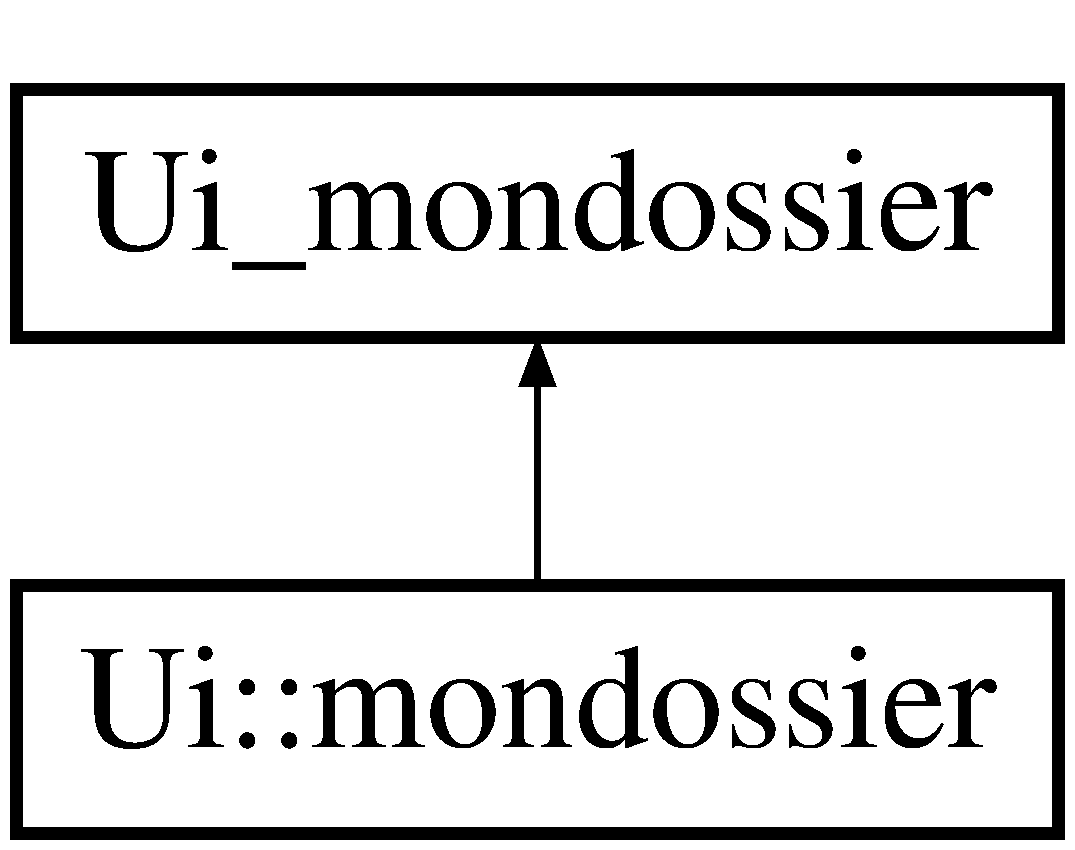
\includegraphics[height=2.000000cm]{class_ui__mondossier}
\end{center}
\end{figure}
\subsection*{Fonctions membres publiques}
\begin{DoxyCompactItemize}
\item 
\hypertarget{class_ui__mondossier_ac4de344ebe23f344d4be204ef04526f5}{void {\bfseries setup\+Ui} (Q\+Dialog $\ast$\hyperlink{classmondossier}{mondossier})}\label{class_ui__mondossier_ac4de344ebe23f344d4be204ef04526f5}

\item 
\hypertarget{class_ui__mondossier_a841ade5774bce5733def3e26bb9f6016}{void {\bfseries retranslate\+Ui} (Q\+Dialog $\ast$\hyperlink{classmondossier}{mondossier})}\label{class_ui__mondossier_a841ade5774bce5733def3e26bb9f6016}

\end{DoxyCompactItemize}
\subsection*{Attributs publics}
\begin{DoxyCompactItemize}
\item 
\hypertarget{class_ui__mondossier_a5e54e2be747afb8ff995c4780637d068}{Q\+Tab\+Widget $\ast$ {\bfseries onglets\+\_\+dossier}}\label{class_ui__mondossier_a5e54e2be747afb8ff995c4780637d068}

\item 
\hypertarget{class_ui__mondossier_a0952bc21ea6b74d97a1330c7314ed114}{Q\+Widget $\ast$ {\bfseries mes\+\_\+infos}}\label{class_ui__mondossier_a0952bc21ea6b74d97a1330c7314ed114}

\item 
\hypertarget{class_ui__mondossier_a1d2ca7632e5cdddbef4af8d664ff667e}{Q\+Label $\ast$ {\bfseries label\+\_\+\+Login}}\label{class_ui__mondossier_a1d2ca7632e5cdddbef4af8d664ff667e}

\item 
\hypertarget{class_ui__mondossier_afb9b84ffb3c7ea778384e3b54b81ad25}{Q\+Label $\ast$ {\bfseries label\+\_\+nom}}\label{class_ui__mondossier_afb9b84ffb3c7ea778384e3b54b81ad25}

\item 
\hypertarget{class_ui__mondossier_a4c40d51ff751021042a973d559e5616e}{Q\+Label $\ast$ {\bfseries label\+\_\+prenom}}\label{class_ui__mondossier_a4c40d51ff751021042a973d559e5616e}

\item 
\hypertarget{class_ui__mondossier_af854695b6e41da3bbb00f19861c574a0}{Q\+Label $\ast$ {\bfseries label\+\_\+date\+\_\+naiss}}\label{class_ui__mondossier_af854695b6e41da3bbb00f19861c574a0}

\item 
\hypertarget{class_ui__mondossier_a113d30eba50e4cd526109510944dc465}{Q\+Label $\ast$ {\bfseries label\+\_\+filiere}}\label{class_ui__mondossier_a113d30eba50e4cd526109510944dc465}

\item 
\hypertarget{class_ui__mondossier_a71ea16436434d942621997f2d3acad72}{Q\+Label $\ast$ {\bfseries label\+\_\+cursus}}\label{class_ui__mondossier_a71ea16436434d942621997f2d3acad72}

\item 
\hypertarget{class_ui__mondossier_ad6c6bbe51a9b1c138ca65725df85fee5}{Q\+Label $\ast$ {\bfseries label\+\_\+branche}}\label{class_ui__mondossier_ad6c6bbe51a9b1c138ca65725df85fee5}

\item 
\hypertarget{class_ui__mondossier_a9ae621df064ef1e4e14e48ebd5a34639}{Q\+Label $\ast$ {\bfseries label\+\_\+sem\+\_\+actu}}\label{class_ui__mondossier_a9ae621df064ef1e4e14e48ebd5a34639}

\item 
\hypertarget{class_ui__mondossier_a71caef553308008a0e82a1eb15a6a62e}{Q\+Label $\ast$ {\bfseries login}}\label{class_ui__mondossier_a71caef553308008a0e82a1eb15a6a62e}

\item 
\hypertarget{class_ui__mondossier_aa0df0d8067da8a915b70a6da11ea96a6}{Q\+Label $\ast$ {\bfseries nom}}\label{class_ui__mondossier_aa0df0d8067da8a915b70a6da11ea96a6}

\item 
\hypertarget{class_ui__mondossier_aa0c368c37d4e76b56498cfbe5f2536e5}{Q\+Label $\ast$ {\bfseries prenom}}\label{class_ui__mondossier_aa0c368c37d4e76b56498cfbe5f2536e5}

\item 
\hypertarget{class_ui__mondossier_aaa0aa6f68959fe6f09f966ff3f9f3a98}{Q\+Label $\ast$ {\bfseries date\+\_\+naiss}}\label{class_ui__mondossier_aaa0aa6f68959fe6f09f966ff3f9f3a98}

\item 
\hypertarget{class_ui__mondossier_acc905a9263b497f5e48098a848e4bbfe}{Q\+Label $\ast$ {\bfseries filiere}}\label{class_ui__mondossier_acc905a9263b497f5e48098a848e4bbfe}

\item 
\hypertarget{class_ui__mondossier_a4928610998dd90ed2754411133d23e52}{Q\+Label $\ast$ {\bfseries cursus}}\label{class_ui__mondossier_a4928610998dd90ed2754411133d23e52}

\item 
\hypertarget{class_ui__mondossier_a236ed8b6c2fdb5bcd6ef2b89d8797a41}{Q\+Label $\ast$ {\bfseries branche}}\label{class_ui__mondossier_a236ed8b6c2fdb5bcd6ef2b89d8797a41}

\item 
\hypertarget{class_ui__mondossier_a41b9a900204ca8f1b0b8e00c42f78352}{Q\+Label $\ast$ {\bfseries semestre}}\label{class_ui__mondossier_a41b9a900204ca8f1b0b8e00c42f78352}

\item 
\hypertarget{class_ui__mondossier_a2409c02e3767705ad0d1f3ed8fc7553a}{Q\+Label $\ast$ {\bfseries label\+\_\+num\+\_\+dossier}}\label{class_ui__mondossier_a2409c02e3767705ad0d1f3ed8fc7553a}

\item 
\hypertarget{class_ui__mondossier_ac60787d38e3bcb4921b02fbcbcf3ccdf}{Q\+Label $\ast$ {\bfseries num\+\_\+dossier}}\label{class_ui__mondossier_ac60787d38e3bcb4921b02fbcbcf3ccdf}

\item 
\hypertarget{class_ui__mondossier_a5d41697944e0a330ea6f1b0b2b4436ea}{Q\+Label $\ast$ {\bfseries email}}\label{class_ui__mondossier_a5d41697944e0a330ea6f1b0b2b4436ea}

\item 
\hypertarget{class_ui__mondossier_a3ec3509fc83d2454e6bdad32dfcda722}{Q\+Label $\ast$ {\bfseries label\+\_\+email}}\label{class_ui__mondossier_a3ec3509fc83d2454e6bdad32dfcda722}

\item 
\hypertarget{class_ui__mondossier_a3bf3cc50f66cc6857f5fe421a3ae5560}{Q\+Label $\ast$ {\bfseries titre\+\_\+mesinfos}}\label{class_ui__mondossier_a3bf3cc50f66cc6857f5fe421a3ae5560}

\item 
\hypertarget{class_ui__mondossier_a1f09bfd5ec8d00b443da0122efbf560e}{Q\+Label $\ast$ {\bfseries fond}}\label{class_ui__mondossier_a1f09bfd5ec8d00b443da0122efbf560e}

\item 
\hypertarget{class_ui__mondossier_a1b78e60c502a40991c2880e4549e4d08}{Q\+Push\+Button $\ast$ {\bfseries sauvegarder\+\_\+modif}}\label{class_ui__mondossier_a1b78e60c502a40991c2880e4549e4d08}

\item 
\hypertarget{class_ui__mondossier_a15921c44dc8d542101ed3a85ba981ee7}{Q\+Line\+Edit $\ast$ {\bfseries modif\+\_\+login}}\label{class_ui__mondossier_a15921c44dc8d542101ed3a85ba981ee7}

\item 
\hypertarget{class_ui__mondossier_a7b3247525abe7e641391390c87d29163}{Q\+Line\+Edit $\ast$ {\bfseries modif\+\_\+nom}}\label{class_ui__mondossier_a7b3247525abe7e641391390c87d29163}

\item 
\hypertarget{class_ui__mondossier_a91c07892365c9d17fc52f84abfec3789}{Q\+Line\+Edit $\ast$ {\bfseries modif\+\_\+date\+\_\+naiss}}\label{class_ui__mondossier_a91c07892365c9d17fc52f84abfec3789}

\item 
\hypertarget{class_ui__mondossier_a3c332ec1dfc727f35d83eb7dbd499d00}{Q\+Line\+Edit $\ast$ {\bfseries modif\+\_\+prenom}}\label{class_ui__mondossier_a3c332ec1dfc727f35d83eb7dbd499d00}

\item 
\hypertarget{class_ui__mondossier_a53484f23d9769a358ecf176000375c21}{Q\+Line\+Edit $\ast$ {\bfseries modif\+\_\+email}}\label{class_ui__mondossier_a53484f23d9769a358ecf176000375c21}

\item 
\hypertarget{class_ui__mondossier_aa0ea2a2f11c3ce1d9c041e9db8536974}{Q\+Push\+Button $\ast$ {\bfseries modif\+\_\+info}}\label{class_ui__mondossier_aa0ea2a2f11c3ce1d9c041e9db8536974}

\item 
\hypertarget{class_ui__mondossier_a56d83b9ea6b4f052db63c4be437f96aa}{Q\+Combo\+Box $\ast$ {\bfseries modif\+\_\+filiere}}\label{class_ui__mondossier_a56d83b9ea6b4f052db63c4be437f96aa}

\item 
\hypertarget{class_ui__mondossier_a1f51afe0be5f2f0d99631db8c27fa667}{Q\+Combo\+Box $\ast$ {\bfseries modif\+\_\+cursus}}\label{class_ui__mondossier_a1f51afe0be5f2f0d99631db8c27fa667}

\item 
\hypertarget{class_ui__mondossier_a6084c44a6a6e672e3fb4f1afa49cf7a2}{Q\+Combo\+Box $\ast$ {\bfseries modif\+\_\+branche}}\label{class_ui__mondossier_a6084c44a6a6e672e3fb4f1afa49cf7a2}

\item 
\hypertarget{class_ui__mondossier_a61fe1fce21338c5517ecbcbd7a1b0979}{Q\+Combo\+Box $\ast$ {\bfseries modif\+\_\+semestre}}\label{class_ui__mondossier_a61fe1fce21338c5517ecbcbd7a1b0979}

\item 
\hypertarget{class_ui__mondossier_a61ec00d1d9468f793a46a528d34b58a9}{Q\+Widget $\ast$ {\bfseries tab\+\_\+info\+\_\+perso}}\label{class_ui__mondossier_a61ec00d1d9468f793a46a528d34b58a9}

\item 
\hypertarget{class_ui__mondossier_a735dfb8b9c899fcf5d90da9eca876569}{Q\+Label $\ast$ {\bfseries label\+\_\+2}}\label{class_ui__mondossier_a735dfb8b9c899fcf5d90da9eca876569}

\item 
\hypertarget{class_ui__mondossier_af876b5a4b8134bd550b3bce21687ebde}{Q\+Label $\ast$ {\bfseries label\+\_\+3}}\label{class_ui__mondossier_af876b5a4b8134bd550b3bce21687ebde}

\item 
\hypertarget{class_ui__mondossier_af99368068216156c33f9a9aaf17f8291}{Q\+Label $\ast$ {\bfseries label\+\_\+4}}\label{class_ui__mondossier_af99368068216156c33f9a9aaf17f8291}

\item 
\hypertarget{class_ui__mondossier_a9c0b42e415b02977c4153229613eecfd}{Q\+Combo\+Box $\ast$ {\bfseries combo\+Box\+\_\+note}}\label{class_ui__mondossier_a9c0b42e415b02977c4153229613eecfd}

\item 
\hypertarget{class_ui__mondossier_a2132b63fadd418d1421705ae5873504d}{Q\+Label $\ast$ {\bfseries label\+\_\+5}}\label{class_ui__mondossier_a2132b63fadd418d1421705ae5873504d}

\item 
\hypertarget{class_ui__mondossier_a86f828454240a36dc530464274510aef}{Q\+Frame $\ast$ {\bfseries line}}\label{class_ui__mondossier_a86f828454240a36dc530464274510aef}

\item 
\hypertarget{class_ui__mondossier_a74ce17d586438c09e2e03de8455fea4c}{Q\+Push\+Button $\ast$ {\bfseries ajout\+\_\+uv}}\label{class_ui__mondossier_a74ce17d586438c09e2e03de8455fea4c}

\item 
\hypertarget{class_ui__mondossier_ae7d2529abb2e80530834bc7b456c9673}{Q\+List\+Widget $\ast$ {\bfseries liste\+\_\+selection\+\_\+\+U\+V}}\label{class_ui__mondossier_ae7d2529abb2e80530834bc7b456c9673}

\item 
\hypertarget{class_ui__mondossier_a2f179634e25690d23bf7a363c243dd04}{Q\+List\+Widget $\ast$ {\bfseries liste\+\_\+uv\+\_\+suivies}}\label{class_ui__mondossier_a2f179634e25690d23bf7a363c243dd04}

\item 
\hypertarget{class_ui__mondossier_addc7d5ff8910010abcc698d75a82c2c3}{Q\+List\+Widget $\ast$ {\bfseries liste\+\_\+notes}}\label{class_ui__mondossier_addc7d5ff8910010abcc698d75a82c2c3}

\item 
\hypertarget{class_ui__mondossier_a2dfb5ee8e13b7a785e1d6b2dc12193c3}{Q\+Label $\ast$ {\bfseries label\+\_\+6}}\label{class_ui__mondossier_a2dfb5ee8e13b7a785e1d6b2dc12193c3}

\item 
\hypertarget{class_ui__mondossier_acf87e49e81e293d548034679561f1410}{Q\+Combo\+Box $\ast$ {\bfseries combo\+Box\+\_\+semestre}}\label{class_ui__mondossier_acf87e49e81e293d548034679561f1410}

\item 
\hypertarget{class_ui__mondossier_a5c35e8473d7f9944e234a1268a85fddf}{Q\+List\+Widget $\ast$ {\bfseries liste\+\_\+semestres}}\label{class_ui__mondossier_a5c35e8473d7f9944e234a1268a85fddf}

\item 
\hypertarget{class_ui__mondossier_a0f1ef177e259113b133bae47afdd64a5}{Q\+Label $\ast$ {\bfseries label\+\_\+7}}\label{class_ui__mondossier_a0f1ef177e259113b133bae47afdd64a5}

\item 
\hypertarget{class_ui__mondossier_a4853b51405e4cbd04f24ca7968bd3cfe}{Q\+Label $\ast$ {\bfseries label\+\_\+8}}\label{class_ui__mondossier_a4853b51405e4cbd04f24ca7968bd3cfe}

\item 
\hypertarget{class_ui__mondossier_ab9026c3809ebbbdcbb01b16d367da7e7}{Q\+Label $\ast$ {\bfseries fond\+\_\+2}}\label{class_ui__mondossier_ab9026c3809ebbbdcbb01b16d367da7e7}

\item 
\hypertarget{class_ui__mondossier_a060f8e38bdb16356e45f32510693354e}{Q\+Combo\+Box $\ast$ {\bfseries combo\+Box\+\_\+credits}}\label{class_ui__mondossier_a060f8e38bdb16356e45f32510693354e}

\item 
\hypertarget{class_ui__mondossier_aa2c9e9bd25ed083408c358b7627ec4d3}{Q\+Label $\ast$ {\bfseries label\+\_\+9}}\label{class_ui__mondossier_aa2c9e9bd25ed083408c358b7627ec4d3}

\item 
\hypertarget{class_ui__mondossier_ae8a13b3e99f7b2b339a1e4195afae94b}{Q\+List\+Widget $\ast$ {\bfseries liste\+\_\+credits}}\label{class_ui__mondossier_ae8a13b3e99f7b2b339a1e4195afae94b}

\item 
\hypertarget{class_ui__mondossier_a6e0abf8fc339d893b961ffa030b2d46b}{Q\+Label $\ast$ {\bfseries label\+\_\+18}}\label{class_ui__mondossier_a6e0abf8fc339d893b961ffa030b2d46b}

\item 
\hypertarget{class_ui__mondossier_a6e9b5a3a69a10dcc81cc07882c089cba}{Q\+Push\+Button $\ast$ {\bfseries sauvegarder\+\_\+dossier}}\label{class_ui__mondossier_a6e9b5a3a69a10dcc81cc07882c089cba}

\item 
\hypertarget{class_ui__mondossier_aa7d3bed0a7ca1700679e1ccc65c60834}{Q\+List\+Widget $\ast$ {\bfseries liste\+\_\+possibilite\+\_\+uv}}\label{class_ui__mondossier_aa7d3bed0a7ca1700679e1ccc65c60834}

\item 
\hypertarget{class_ui__mondossier_acbdd8bcb6fbb11c11d3d9a135db4e2e5}{Q\+Push\+Button $\ast$ {\bfseries suppri\+\_\+\+U\+V\+\_\+suivies}}\label{class_ui__mondossier_acbdd8bcb6fbb11c11d3d9a135db4e2e5}

\item 
\hypertarget{class_ui__mondossier_a02348ae35448e8b6e509a9cc87cf2dae}{Q\+Group\+Box $\ast$ {\bfseries group\+\_\+criteres\+\_\+recherche}}\label{class_ui__mondossier_a02348ae35448e8b6e509a9cc87cf2dae}

\item 
\hypertarget{class_ui__mondossier_a07787c825b6e3bec7978d93a1f921703}{Q\+Label $\ast$ {\bfseries label\+\_\+cursus\+\_\+2}}\label{class_ui__mondossier_a07787c825b6e3bec7978d93a1f921703}

\item 
\hypertarget{class_ui__mondossier_a35b92e2df9a1064c2a75ee1e5c33190a}{Q\+Label $\ast$ {\bfseries label\+\_\+filiere\+\_\+2}}\label{class_ui__mondossier_a35b92e2df9a1064c2a75ee1e5c33190a}

\item 
\hypertarget{class_ui__mondossier_ac1ef82f23a79becd869025c856f77d98}{Q\+Label $\ast$ {\bfseries label\+\_\+branche\+\_\+2}}\label{class_ui__mondossier_ac1ef82f23a79becd869025c856f77d98}

\item 
\hypertarget{class_ui__mondossier_a4866e36234d6ed8d096c2eea728839dc}{Q\+Combo\+Box $\ast$ {\bfseries combo\+Box\+\_\+cursus}}\label{class_ui__mondossier_a4866e36234d6ed8d096c2eea728839dc}

\item 
\hypertarget{class_ui__mondossier_a5405f59c962d2de52074459dea302a2f}{Q\+Combo\+Box $\ast$ {\bfseries combo\+Box\+\_\+filiere}}\label{class_ui__mondossier_a5405f59c962d2de52074459dea302a2f}

\item 
\hypertarget{class_ui__mondossier_a32b2bde2b56aa25a7afa43eb707a0c93}{Q\+Combo\+Box $\ast$ {\bfseries combo\+Box\+\_\+branche}}\label{class_ui__mondossier_a32b2bde2b56aa25a7afa43eb707a0c93}

\item 
\hypertarget{class_ui__mondossier_aaf6723ac937d078ef42f53d5cc7816a4}{Q\+Widget $\ast$ {\bfseries choix}}\label{class_ui__mondossier_aaf6723ac937d078ef42f53d5cc7816a4}

\item 
\hypertarget{class_ui__mondossier_adb194476b80b0bd7bf3c02d3850234af}{Q\+Push\+Button $\ast$ {\bfseries add\+\_\+exigence}}\label{class_ui__mondossier_adb194476b80b0bd7bf3c02d3850234af}

\item 
\hypertarget{class_ui__mondossier_a100e1a63bdeb3c968cf3f576038af05a}{Q\+Label $\ast$ {\bfseries label\+\_\+titre\+\_\+choix}}\label{class_ui__mondossier_a100e1a63bdeb3c968cf3f576038af05a}

\item 
\hypertarget{class_ui__mondossier_a6ccc3546f055b41a090ad04b1207bec4}{Q\+List\+Widget $\ast$ {\bfseries liste\+\_\+choix\+\_\+uv}}\label{class_ui__mondossier_a6ccc3546f055b41a090ad04b1207bec4}

\item 
\hypertarget{class_ui__mondossier_ac2a27202a40dabe49b5f5e5f7ef84b34}{Q\+List\+Widget $\ast$ {\bfseries liste\+\_\+exigences}}\label{class_ui__mondossier_ac2a27202a40dabe49b5f5e5f7ef84b34}

\item 
\hypertarget{class_ui__mondossier_ac5349692b02d54e553f1ce19cab0a0a5}{Q\+Label $\ast$ {\bfseries label\+\_\+selection\+\_\+uv}}\label{class_ui__mondossier_ac5349692b02d54e553f1ce19cab0a0a5}

\item 
\hypertarget{class_ui__mondossier_ad888c727f20158f653b9177c1d905cbd}{Q\+List\+Widget $\ast$ {\bfseries liste\+\_\+preferences}}\label{class_ui__mondossier_ad888c727f20158f653b9177c1d905cbd}

\item 
\hypertarget{class_ui__mondossier_ad522f665fe4d3312bcaab3c2b1393809}{Q\+List\+Widget $\ast$ {\bfseries liste\+\_\+rejets}}\label{class_ui__mondossier_ad522f665fe4d3312bcaab3c2b1393809}

\item 
\hypertarget{class_ui__mondossier_a171679d4c318a36aede5a799b358bdcc}{Q\+Label $\ast$ {\bfseries label\+\_\+exigences}}\label{class_ui__mondossier_a171679d4c318a36aede5a799b358bdcc}

\item 
\hypertarget{class_ui__mondossier_a55c3f561519adf26068b094d92282b68}{Q\+Label $\ast$ {\bfseries label\+\_\+preferences}}\label{class_ui__mondossier_a55c3f561519adf26068b094d92282b68}

\item 
\hypertarget{class_ui__mondossier_a97e823e0f049621fe318280b477b129d}{Q\+Label $\ast$ {\bfseries label\+\_\+rejets}}\label{class_ui__mondossier_a97e823e0f049621fe318280b477b129d}

\item 
\hypertarget{class_ui__mondossier_a94b79690ddd4c65b5c68fff4b3d2e091}{Q\+Push\+Button $\ast$ {\bfseries sauvegarder\+\_\+choix}}\label{class_ui__mondossier_a94b79690ddd4c65b5c68fff4b3d2e091}

\item 
\hypertarget{class_ui__mondossier_add6610f42b207d0faf300d28e8907138}{Q\+Push\+Button $\ast$ {\bfseries add\+\_\+preference}}\label{class_ui__mondossier_add6610f42b207d0faf300d28e8907138}

\item 
\hypertarget{class_ui__mondossier_ad308f3c9bf0d12827aa56d44b54a2bb1}{Q\+Push\+Button $\ast$ {\bfseries add\+\_\+rejet}}\label{class_ui__mondossier_ad308f3c9bf0d12827aa56d44b54a2bb1}

\item 
\hypertarget{class_ui__mondossier_a9646776bf491dffcb936d8b5909af695}{Q\+Push\+Button $\ast$ {\bfseries suppr\+\_\+exigence}}\label{class_ui__mondossier_a9646776bf491dffcb936d8b5909af695}

\item 
\hypertarget{class_ui__mondossier_ae6357c71d6b93abf264298fa79309a15}{Q\+Push\+Button $\ast$ {\bfseries suppr\+\_\+preference}}\label{class_ui__mondossier_ae6357c71d6b93abf264298fa79309a15}

\item 
\hypertarget{class_ui__mondossier_a698c2d3ec121ece0161f242701b97a5a}{Q\+Push\+Button $\ast$ {\bfseries suppr\+\_\+rejet}}\label{class_ui__mondossier_a698c2d3ec121ece0161f242701b97a5a}

\item 
\hypertarget{class_ui__mondossier_a5dc5440eb9874075a4796d5d97ee5f43}{Q\+Label $\ast$ {\bfseries fond\+\_\+3}}\label{class_ui__mondossier_a5dc5440eb9874075a4796d5d97ee5f43}

\item 
\hypertarget{class_ui__mondossier_a452a7091d72ee139c8c5e70ba32299ce}{Q\+Push\+Button $\ast$ {\bfseries suggestion\+\_\+uv}}\label{class_ui__mondossier_a452a7091d72ee139c8c5e70ba32299ce}

\item 
\hypertarget{class_ui__mondossier_a9f58e528e4e62cbd5d3d0b5e7b79177d}{Q\+Label $\ast$ {\bfseries label}}\label{class_ui__mondossier_a9f58e528e4e62cbd5d3d0b5e7b79177d}

\end{DoxyCompactItemize}


La documentation de cette classe a été générée à partir du fichier suivant \+:\begin{DoxyCompactItemize}
\item 
ui\+\_\+mondossier.\+h\end{DoxyCompactItemize}

\hypertarget{class_ui___view_uv}{\section{Référence de la classe Ui\+\_\+\+View\+Uv}
\label{class_ui___view_uv}\index{Ui\+\_\+\+View\+Uv@{Ui\+\_\+\+View\+Uv}}
}
Graphe d'héritage de Ui\+\_\+\+View\+Uv\+:\begin{figure}[H]
\begin{center}
\leavevmode
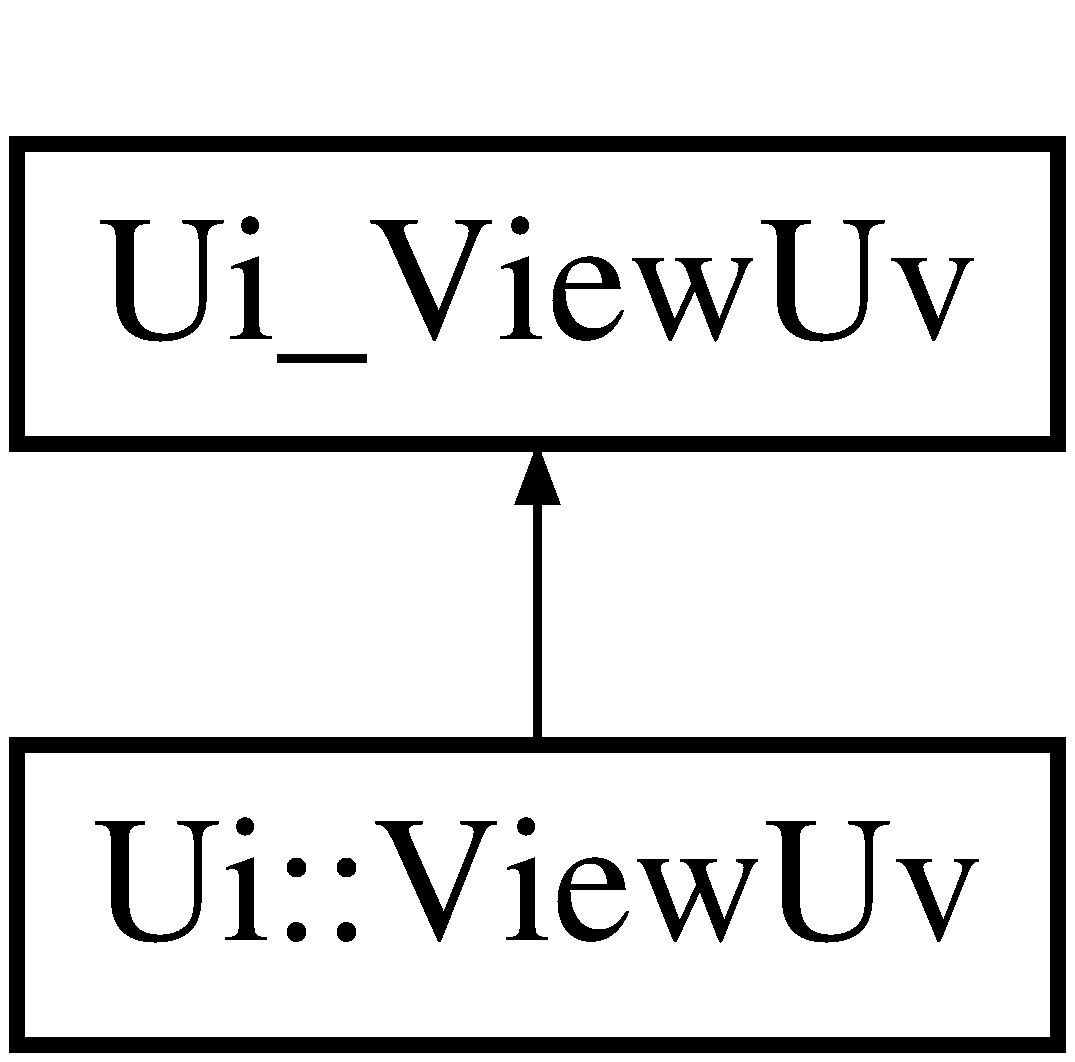
\includegraphics[height=2.000000cm]{class_ui___view_uv}
\end{center}
\end{figure}
\subsection*{Fonctions membres publiques}
\begin{DoxyCompactItemize}
\item 
\hypertarget{class_ui___view_uv_a0a1d76d53d9d126148dcdfa53953b071}{void {\bfseries setup\+Ui} (Q\+Widget $\ast$\hyperlink{class_view_uv}{View\+Uv})}\label{class_ui___view_uv_a0a1d76d53d9d126148dcdfa53953b071}

\item 
\hypertarget{class_ui___view_uv_ab8028a558494c465f8ecfcd961548f6e}{void {\bfseries retranslate\+Ui} (Q\+Widget $\ast$\hyperlink{class_view_uv}{View\+Uv})}\label{class_ui___view_uv_ab8028a558494c465f8ecfcd961548f6e}

\end{DoxyCompactItemize}
\subsection*{Attributs publics}
\begin{DoxyCompactItemize}
\item 
\hypertarget{class_ui___view_uv_ac0e008871ce7fcf9b24d3ee970918ba8}{Q\+Tab\+Widget $\ast$ {\bfseries tab\+Widget}}\label{class_ui___view_uv_ac0e008871ce7fcf9b24d3ee970918ba8}

\item 
\hypertarget{class_ui___view_uv_ad1695fcce562e6a3f90aa8aea679fe16}{Q\+Widget $\ast$ {\bfseries Tout}}\label{class_ui___view_uv_ad1695fcce562e6a3f90aa8aea679fe16}

\item 
\hypertarget{class_ui___view_uv_a1fae3922ba661d981f25ee5f3f660d52}{Q\+List\+Widget $\ast$ {\bfseries all\+Uv}}\label{class_ui___view_uv_a1fae3922ba661d981f25ee5f3f660d52}

\end{DoxyCompactItemize}


La documentation de cette classe a été générée à partir du fichier suivant \+:\begin{DoxyCompactItemize}
\item 
ui\+\_\+viewuv.\+h\end{DoxyCompactItemize}

\hypertarget{class_u_t_profiler_exception}{\section{Référence de la classe U\+T\+Profiler\+Exception}
\label{class_u_t_profiler_exception}\index{U\+T\+Profiler\+Exception@{U\+T\+Profiler\+Exception}}
}
\subsection*{Fonctions membres publiques}
\begin{DoxyCompactItemize}
\item 
\hypertarget{class_u_t_profiler_exception_afd289268648bada41417156ceb1269fd}{{\bfseries U\+T\+Profiler\+Exception} (const Q\+String \&message, const Q\+String \&f=\char`\"{}na\char`\"{}, unsigned int l=0)}\label{class_u_t_profiler_exception_afd289268648bada41417156ceb1269fd}

\item 
\hypertarget{class_u_t_profiler_exception_a6f4582234c00b4fe67776ef10c5370bf}{Q\+String {\bfseries get\+Info} () const }\label{class_u_t_profiler_exception_a6f4582234c00b4fe67776ef10c5370bf}

\item 
\hypertarget{class_u_t_profiler_exception_ae54e6a5c0836dcc62fee879651ae5679}{Q\+String {\bfseries get\+File} () const }\label{class_u_t_profiler_exception_ae54e6a5c0836dcc62fee879651ae5679}

\item 
\hypertarget{class_u_t_profiler_exception_aa3c2efb28c6b482859b26b8f59b4b32e}{unsigned int {\bfseries get\+Line} () const }\label{class_u_t_profiler_exception_aa3c2efb28c6b482859b26b8f59b4b32e}

\end{DoxyCompactItemize}


La documentation de cette classe a été générée à partir du fichier suivant \+:\begin{DoxyCompactItemize}
\item 
utprofilerexception.\+h\end{DoxyCompactItemize}

\hypertarget{class_u_v}{\section{Référence de la classe U\+V}
\label{class_u_v}\index{U\+V@{U\+V}}
}
\subsection*{Fonctions membres publiques}
\begin{DoxyCompactItemize}
\item 
\hypertarget{class_u_v_a4d5fe39505b3e474b41013dda0d2047a}{Q\+String {\bfseries get\+Code} () const }\label{class_u_v_a4d5fe39505b3e474b41013dda0d2047a}

\item 
\hypertarget{class_u_v_afa7f5a8c7ea21bedcd00af1a1ff48221}{Q\+String {\bfseries get\+Titre} () const }\label{class_u_v_afa7f5a8c7ea21bedcd00af1a1ff48221}

\item 
\hypertarget{class_u_v_a68c71544276792a5cf8de0b146830eaa}{unsigned int {\bfseries get\+Nb\+Credits} () const }\label{class_u_v_a68c71544276792a5cf8de0b146830eaa}

\item 
\hypertarget{class_u_v_ab57e190abc1bce79c34a0ad457a920a6}{\hyperlink{class_categorie}{Categorie} {\bfseries get\+Categorie} () const }\label{class_u_v_ab57e190abc1bce79c34a0ad457a920a6}

\item 
\hypertarget{class_u_v_a29423fb485037fc882b8b29cae033c9a}{bool {\bfseries ouverture\+Automne} () const }\label{class_u_v_a29423fb485037fc882b8b29cae033c9a}

\item 
\hypertarget{class_u_v_adca45078b74fdc3c09621a521756e8af}{bool {\bfseries ouverture\+Printemps} () const }\label{class_u_v_adca45078b74fdc3c09621a521756e8af}

\item 
\hypertarget{class_u_v_a9c3b73077819774423559abd838e410b}{void {\bfseries set\+Code} (const Q\+String \&c)}\label{class_u_v_a9c3b73077819774423559abd838e410b}

\item 
\hypertarget{class_u_v_a52c66013e137689883802465596bb688}{void {\bfseries set\+Titre} (const Q\+String \&t)}\label{class_u_v_a52c66013e137689883802465596bb688}

\item 
\hypertarget{class_u_v_afe8639c00d1314a9f329385835771eef}{void {\bfseries set\+Nb\+Credits} (unsigned int n)}\label{class_u_v_afe8639c00d1314a9f329385835771eef}

\item 
\hypertarget{class_u_v_a8bf3d3307d4e7f7f5284085d1bc07262}{void {\bfseries set\+Categorie} (\hyperlink{class_categorie}{Categorie} c)}\label{class_u_v_a8bf3d3307d4e7f7f5284085d1bc07262}

\item 
\hypertarget{class_u_v_a7e670e649febebe0fe70c3ce79f4be63}{void {\bfseries set\+Ouverture\+Automne} (bool b)}\label{class_u_v_a7e670e649febebe0fe70c3ce79f4be63}

\item 
\hypertarget{class_u_v_a0ae246826809cc48a1999ec0671c78b3}{void {\bfseries set\+Ouverture\+Printemps} (bool b)}\label{class_u_v_a0ae246826809cc48a1999ec0671c78b3}

\end{DoxyCompactItemize}
\subsection*{Amis}
\begin{DoxyCompactItemize}
\item 
\hypertarget{class_u_v_a335ec2026467669b89518b0c67372f3b}{class {\bfseries U\+V\+Manager}}\label{class_u_v_a335ec2026467669b89518b0c67372f3b}

\end{DoxyCompactItemize}


La documentation de cette classe a été générée à partir du fichier suivant \+:\begin{DoxyCompactItemize}
\item 
uv.\+h\end{DoxyCompactItemize}

\hypertarget{class_u_v_manager}{\section{Référence de la classe U\+V\+Manager}
\label{class_u_v_manager}\index{U\+V\+Manager@{U\+V\+Manager}}
}
\subsection*{Classes}
\begin{DoxyCompactItemize}
\item 
class \hyperlink{class_u_v_manager_1_1_filter_iterator}{Filter\+Iterator}
\item 
class \hyperlink{class_u_v_manager_1_1iterator}{iterator}
\item 
class \hyperlink{class_u_v_manager_1_1_iterator}{Iterator}
\end{DoxyCompactItemize}
\subsection*{Fonctions membres publiques}
\begin{DoxyCompactItemize}
\item 
\hypertarget{class_u_v_manager_a60556f66f72f41786ffb70f066f1a846}{void {\bfseries load} (const Q\+String \&f)}\label{class_u_v_manager_a60556f66f72f41786ffb70f066f1a846}

\item 
\hypertarget{class_u_v_manager_a1e52ce1b69c6239d19016ec3cb74bd1c}{void {\bfseries save} (const Q\+String \&f)}\label{class_u_v_manager_a1e52ce1b69c6239d19016ec3cb74bd1c}

\item 
\hypertarget{class_u_v_manager_ae356bbc490312c58a02d2b00afee8fc3}{void {\bfseries ajouter\+U\+V} (const Q\+String \&c, const Q\+String \&t, unsigned int nbc, \hyperlink{class_categorie}{Categorie} cat, bool a, bool p)}\label{class_u_v_manager_ae356bbc490312c58a02d2b00afee8fc3}

\item 
\hypertarget{class_u_v_manager_a34b0938d1c9100068d8ecfbf56b1288e}{const \hyperlink{class_u_v}{U\+V} \& {\bfseries get\+U\+V} (const Q\+String \&code) const }\label{class_u_v_manager_a34b0938d1c9100068d8ecfbf56b1288e}

\item 
\hypertarget{class_u_v_manager_a72b706433904db6209179dc60c4d0d2e}{\hyperlink{class_u_v}{U\+V} \& {\bfseries get\+U\+V} (const Q\+String \&code)}\label{class_u_v_manager_a72b706433904db6209179dc60c4d0d2e}

\item 
\hypertarget{class_u_v_manager_a8ed63e00fc4d07be00fcbbb8b542de78}{\hyperlink{class_u_v_manager_1_1_iterator}{Iterator} {\bfseries get\+Iterator} ()}\label{class_u_v_manager_a8ed63e00fc4d07be00fcbbb8b542de78}

\item 
\hypertarget{class_u_v_manager_aecc02d7bc30df5dedc407c50236b250b}{\hyperlink{class_u_v_manager_1_1iterator}{iterator} {\bfseries begin} ()}\label{class_u_v_manager_aecc02d7bc30df5dedc407c50236b250b}

\item 
\hypertarget{class_u_v_manager_a13466f9977fb20fb018a5cd288d4b9a4}{\hyperlink{class_u_v_manager_1_1iterator}{iterator} {\bfseries end} ()}\label{class_u_v_manager_a13466f9977fb20fb018a5cd288d4b9a4}

\item 
\hypertarget{class_u_v_manager_a6c08405fd5dff4b92ccdb8ab60aca58a}{\hyperlink{class_u_v_manager_1_1_filter_iterator}{Filter\+Iterator} {\bfseries get\+Filter\+Iterator} (\hyperlink{class_categorie}{Categorie} c)}\label{class_u_v_manager_a6c08405fd5dff4b92ccdb8ab60aca58a}

\end{DoxyCompactItemize}
\subsection*{Fonctions membres publiques statiques}
\begin{DoxyCompactItemize}
\item 
\hypertarget{class_u_v_manager_ac3a0dd0ffad43b2c6a39df72b58d2bb4}{static \hyperlink{class_u_v_manager}{U\+V\+Manager} \& {\bfseries get\+Instance} ()}\label{class_u_v_manager_ac3a0dd0ffad43b2c6a39df72b58d2bb4}

\item 
\hypertarget{class_u_v_manager_a3a547b31583aa76df3056ea32b9f9776}{static void {\bfseries liberer\+Instance} ()}\label{class_u_v_manager_a3a547b31583aa76df3056ea32b9f9776}

\end{DoxyCompactItemize}
\subsection*{Amis}
\begin{DoxyCompactItemize}
\item 
\hypertarget{class_u_v_manager_a7ab9a1e3d1a8ab9a8badf544bf7e0197}{struct {\bfseries Handler}}\label{class_u_v_manager_a7ab9a1e3d1a8ab9a8badf544bf7e0197}

\end{DoxyCompactItemize}


La documentation de cette classe a été générée à partir du fichier suivant \+:\begin{DoxyCompactItemize}
\item 
uvmanager.\+h\end{DoxyCompactItemize}

\hypertarget{classuvmnger}{\section{Référence de la classe uvmnger}
\label{classuvmnger}\index{uvmnger@{uvmnger}}
}
Graphe d'héritage de uvmnger\+:\begin{figure}[H]
\begin{center}
\leavevmode
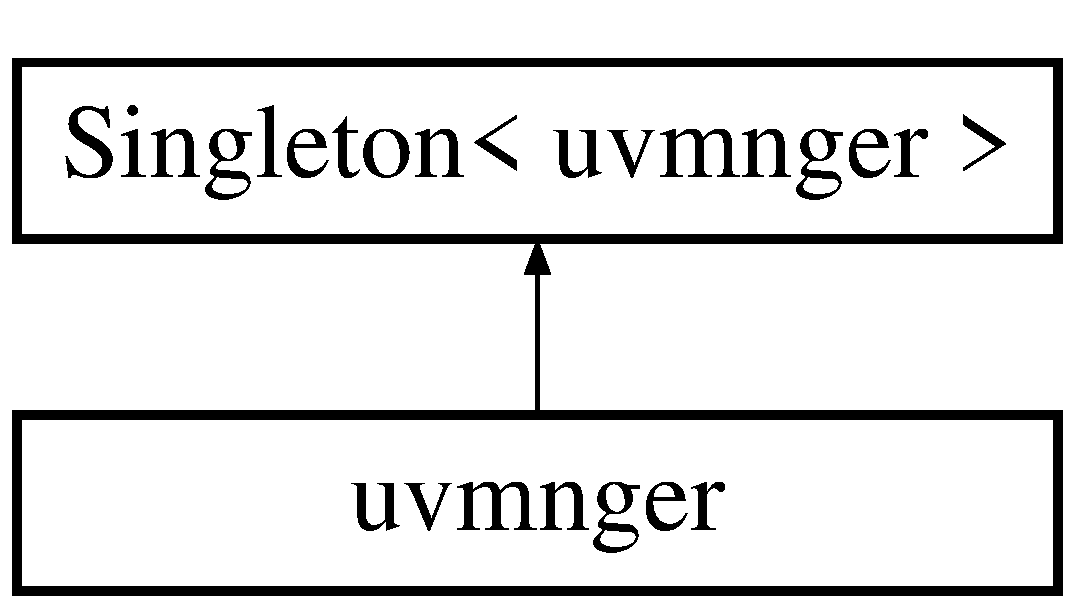
\includegraphics[height=2.000000cm]{classuvmnger}
\end{center}
\end{figure}
\subsection*{Fonctions membres publiques}
\begin{DoxyCompactItemize}
\item 
\hypertarget{classuvmnger_a16ac6c78fdab0151ec2685a12c78c7e6}{map$<$ Q\+String, Q\+String $>$ {\bfseries get\+Possibilite\+From\+Uv} (const Q\+String \&Uv)}\label{classuvmnger_a16ac6c78fdab0151ec2685a12c78c7e6}

\end{DoxyCompactItemize}
\subsection*{Amis}
\begin{DoxyCompactItemize}
\item 
\hypertarget{classuvmnger_a162f1ec43266b7dc7d1dfcee3c3a6a0e}{class {\bfseries Singleton$<$ uvmnger $>$}}\label{classuvmnger_a162f1ec43266b7dc7d1dfcee3c3a6a0e}

\end{DoxyCompactItemize}
\subsection*{Membres hérités additionnels}


La documentation de cette classe a été générée à partir des fichiers suivants \+:\begin{DoxyCompactItemize}
\item 
uvmnger.\+h\item 
uvmnger.\+cpp\end{DoxyCompactItemize}

\hypertarget{class_ui_1_1_view_uv}{\section{Référence de la classe Ui\+:\+:View\+Uv}
\label{class_ui_1_1_view_uv}\index{Ui\+::\+View\+Uv@{Ui\+::\+View\+Uv}}
}
Graphe d'héritage de Ui\+:\+:View\+Uv\+:\begin{figure}[H]
\begin{center}
\leavevmode
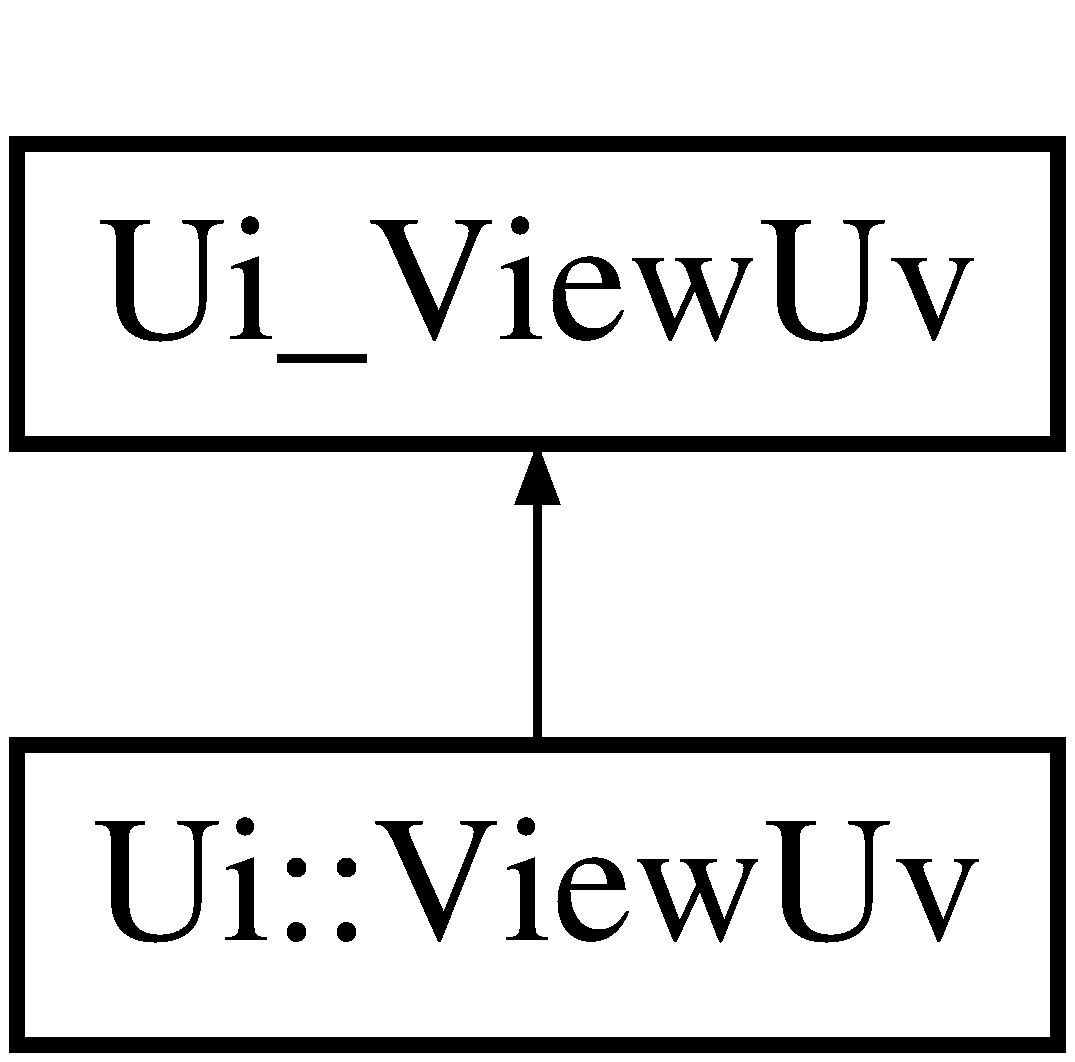
\includegraphics[height=2.000000cm]{class_ui_1_1_view_uv}
\end{center}
\end{figure}
\subsection*{Membres hérités additionnels}


La documentation de cette classe a été générée à partir du fichier suivant \+:\begin{DoxyCompactItemize}
\item 
ui\+\_\+viewuv.\+h\end{DoxyCompactItemize}

\hypertarget{class_view_uv}{\section{Référence de la classe View\+Uv}
\label{class_view_uv}\index{View\+Uv@{View\+Uv}}
}
Graphe d'héritage de View\+Uv\+:\begin{figure}[H]
\begin{center}
\leavevmode
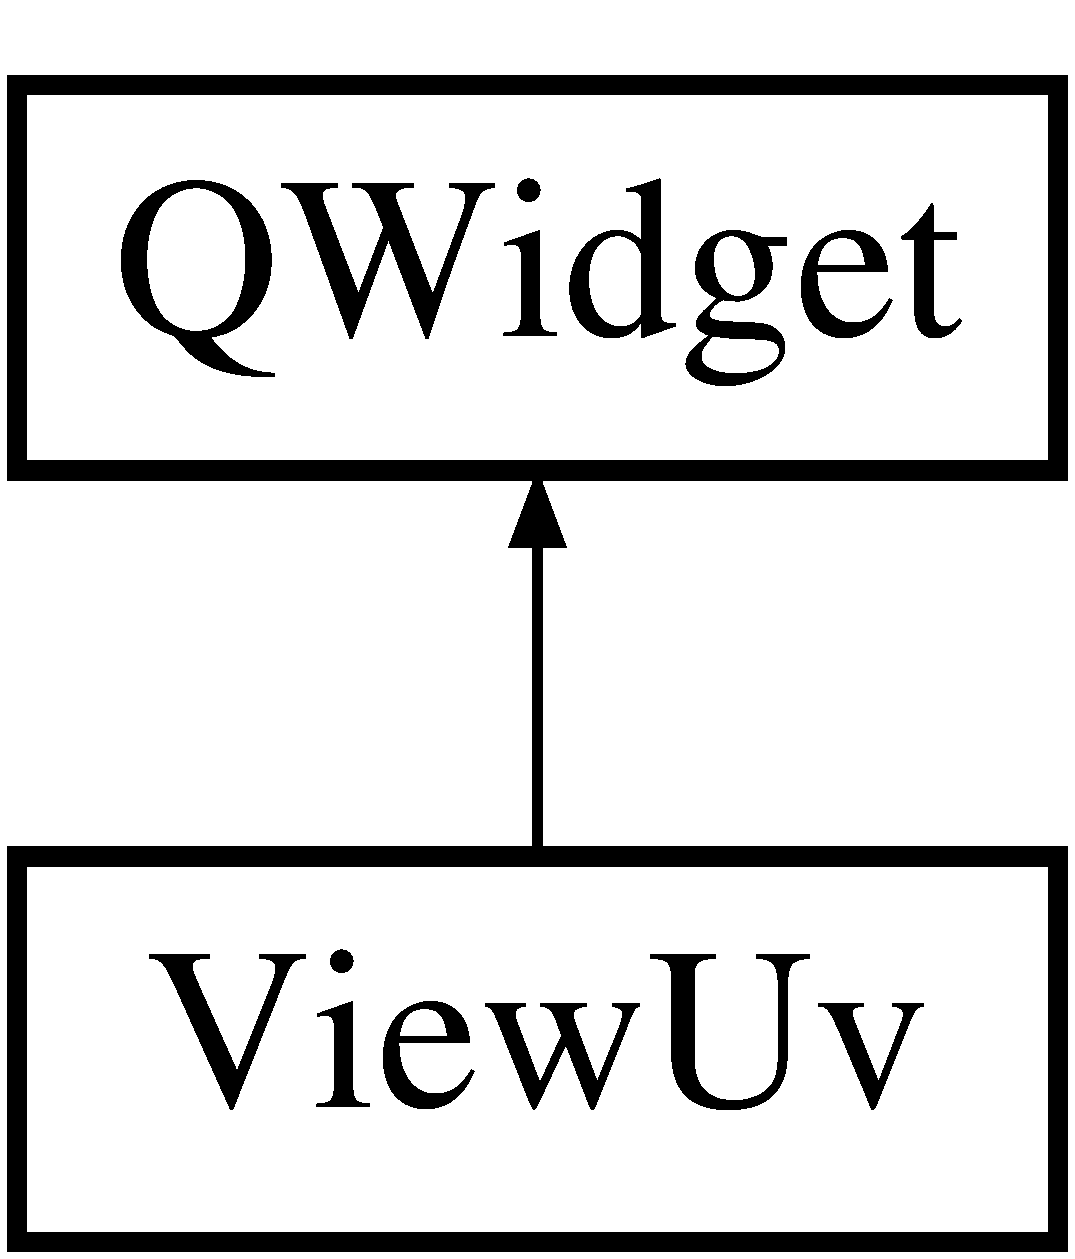
\includegraphics[height=2.000000cm]{class_view_uv}
\end{center}
\end{figure}
\subsection*{Fonctions membres publiques}
\begin{DoxyCompactItemize}
\item 
\hypertarget{class_view_uv_a234d80938d244e3682470a86463a9195}{{\bfseries View\+Uv} (Q\+Widget $\ast$parent=0)}\label{class_view_uv_a234d80938d244e3682470a86463a9195}

\end{DoxyCompactItemize}


La documentation de cette classe a été générée à partir des fichiers suivants \+:\begin{DoxyCompactItemize}
\item 
viewuv.\+h\item 
viewuv.\+cpp\end{DoxyCompactItemize}

\chapter{Documentation des fichiers}
\hypertarget{accueil_8cpp}{\section{Référence du fichier accueil.\+cpp}
\label{accueil_8cpp}\index{accueil.\+cpp@{accueil.\+cpp}}
}
{\ttfamily \#include \char`\"{}accueil.\+h\char`\"{}}\\*
{\ttfamily \#include \char`\"{}ui\+\_\+accueil.\+h\char`\"{}}\\*

\hypertarget{accueil_8h}{\section{Référence du fichier accueil.\+h}
\label{accueil_8h}\index{accueil.\+h@{accueil.\+h}}
}


Interface d'accueil de l'application.  


{\ttfamily \#include $<$Q\+Layout$>$}\\*
{\ttfamily \#include $<$Q\+Main\+Window$>$}\\*
{\ttfamily \#include $<$Q\+List\+Widget$>$}\\*
{\ttfamily \#include $<$Q\+Check\+Box$>$}\\*
{\ttfamily \#include $<$Q\+Group\+Box$>$}\\*
{\ttfamily \#include $<$Q\+Push\+Button$>$}\\*
{\ttfamily \#include $<$Q\+Map$>$}\\*
{\ttfamily \#include \char`\"{}connexion.\+h\char`\"{}}\\*
{\ttfamily \#include \char`\"{}inscription.\+h\char`\"{}}\\*
{\ttfamily \#include \char`\"{}dbmanager.\+h\char`\"{}}\\*
{\ttfamily \#include \char`\"{}utprofilerexception.\+h\char`\"{}}\\*
{\ttfamily \#include \char`\"{}formulaire.\+h\char`\"{}}\\*
{\ttfamily \#include \char`\"{}mondossier.\+h\char`\"{}}\\*
{\ttfamily \#include \char`\"{}cursus.\+h\char`\"{}}\\*
{\ttfamily \#include \char`\"{}administration.\+h\char`\"{}}\\*
\subsection*{Classes}
\begin{DoxyCompactItemize}
\item 
class \hyperlink{class_accueil}{Accueil}
\end{DoxyCompactItemize}


\subsection{Description détaillée}
Interface d'accueil de l'application. 


\hypertarget{administration_8cpp}{\section{Référence du fichier administration.\+cpp}
\label{administration_8cpp}\index{administration.\+cpp@{administration.\+cpp}}
}
{\ttfamily \#include \char`\"{}administration.\+h\char`\"{}}\\*
{\ttfamily \#include \char`\"{}ui\+\_\+administration.\+h\char`\"{}}\\*

\hypertarget{administration_8h}{\section{Référence du fichier administration.\+h}
\label{administration_8h}\index{administration.\+h@{administration.\+h}}
}
{\ttfamily \#include $<$Q\+Frame$>$}\\*
{\ttfamily \#include \char`\"{}dbmanager.\+h\char`\"{}}\\*
{\ttfamily \#include \char`\"{}formulaire.\+h\char`\"{}}\\*
{\ttfamily \#include $<$Q\+List\+Widget$>$}\\*
{\ttfamily \#include \char`\"{}utprofilerexception.\+h\char`\"{}}\\*
{\ttfamily \#include \char`\"{}cursus.\+h\char`\"{}}\\*
{\ttfamily \#include \char`\"{}branches.\+h\char`\"{}}\\*
{\ttfamily \#include \char`\"{}filieres.\+h\char`\"{}}\\*
{\ttfamily \#include \char`\"{}categorie.\+h\char`\"{}}\\*
{\ttfamily \#include \char`\"{}disponibilites.\+h\char`\"{}}\\*
{\ttfamily \#include \char`\"{}etudiants.\+h\char`\"{}}\\*
{\ttfamily \#include $<$Q\+Message\+Box$>$}\\*
{\ttfamily \#include \char`\"{}tools.\+h\char`\"{}}\\*
\subsection*{Classes}
\begin{DoxyCompactItemize}
\item 
class \hyperlink{class_administration}{Administration}
\end{DoxyCompactItemize}

\hypertarget{main_8cpp}{\section{Référence du fichier main.\+cpp}
\label{main_8cpp}\index{main.\+cpp@{main.\+cpp}}
}
{\ttfamily \#include \char`\"{}dbmanager.\+h\char`\"{}}\\*
{\ttfamily \#include $<$Q\+Application$>$}\\*
{\ttfamily \#include \char`\"{}accueil.\+h\char`\"{}}\\*
{\ttfamily \#include \char`\"{}filieres.\+h\char`\"{}}\\*
\subsection*{Fonctions}
\begin{DoxyCompactItemize}
\item 
int \hyperlink{main_8cpp_a0ddf1224851353fc92bfbff6f499fa97}{main} (int argc, char $\ast$argv\mbox{[}$\,$\mbox{]})
\begin{DoxyCompactList}\small\item\em Entrée du programme. \end{DoxyCompactList}\end{DoxyCompactItemize}


\subsection{Description détaillée}
\begin{DoxyAuthor}{Auteur}
David Martins 

Benoît Sénéchal 
\end{DoxyAuthor}
\begin{DoxyVersion}{Version}
1.\+0 
\end{DoxyVersion}
\begin{DoxyDate}{Date}
15 Juin 2014 
\end{DoxyDate}


\subsection{Documentation des fonctions}
\hypertarget{main_8cpp_a0ddf1224851353fc92bfbff6f499fa97}{\index{main.\+cpp@{main.\+cpp}!main@{main}}
\index{main@{main}!main.\+cpp@{main.\+cpp}}
\subsubsection[{main}]{\setlength{\rightskip}{0pt plus 5cm}int main (
\begin{DoxyParamCaption}
\item[{int}]{argc, }
\item[{char $\ast$}]{argv\mbox{[}$\,$\mbox{]}}
\end{DoxyParamCaption}
)}}\label{main_8cpp_a0ddf1224851353fc92bfbff6f499fa97}


Entrée du programme. 

\begin{DoxyReturn}{Renvoie}
app.\+exec() -\/ Arrêt normal du programme. 
\end{DoxyReturn}
Initialisation de la B\+D\+D 
%--- End generated contents ---

% Index
\newpage
\phantomsection
\addcontentsline{toc}{chapter}{Index}
\printindex

\end{document}
